\documentclass[12pt]{uthesis-v12}  %---> DO NOT ALTER THIS COMMAND

\usepackage{graphicx}

% *** GRAPHICS RELATED PACKAGES ***
%
%\ifCLASSINFOpdf
 % \usepackage[pdftex]{graphicx}
  % declare the path(s) where your graphic files are
\graphicspath{{figures/pdf/}{figures/eps/}}
  % and their extensions so you won't have to specify these with
  % every instance of \includegraphics
  %\DeclareGraphicsExtensions{.pdf,.jpeg,.png}
%\else
  % or other class option (dvipsone, dvipdf, if not using dvips). graphicx
  % will default to the driver specified in the system graphics.cfg if no
  % driver is specified.
 % \usepackage[dvips]{graphicx}
  % declare the path(s) where your graphic files are
  %\graphicspath{{../eps/}}
  % and their extensions so you won't have to specify these with
  % every instance of \includegraphics
  %\DeclareGraphicsExtensions{.eps}
%\fi

\usepackage{mathtools}

\usepackage{subfig}
\usepackage{algorithmic}
\usepackage{booktabs}
\usepackage{epstopdf}
\usepackage[T1]{fontenc}

\usepackage{array}
\newcolumntype{L}[1]{>{\raggedright\let\newline\\\arraybackslash\hspace{0pt}}m{#1}}

\renewcommand{\arraystretch}{1.2}

\usepackage{float}
\newfloat{algorithm}{t}{lop}
\floatname{algorithm}{Algorithm}
\usepackage{xpatch}

\usepackage{accents}
\newcommand{\ubar}[1]{\underaccent{\bar}{#1}}



%% The amssymb package provides various useful mathematical symbols
\usepackage{amssymb}
\usepackage{cleveref}


\usepackage[labelsep=colon]
                %labelfont={sf,bf},
                %textfont=sf]
               {caption}

%\makeatletter
%\xpatchcmd{\algorithmic}{\itemsep\z@}{\itemsep=1ex plus0.5pt}{}{}
%\makeatother

\begin{document} %---> %---> %---> %---> DO NOT ALTER THIS COMMAND

%--------+----------------------------------------------------------+
%        |  \title{}                                    (REQUIRED)  |
%        |  \author{}                                   (REQUIRED)  |
%        |                                                          |
%        |  See section 3.1 of "Read_Me_First_(v12).pdf"            |
%        |                                                          |
%        |  Also see section 2.2 of above "Read Me" file for the    |
%        |  proper use of the invisible tilde ("~") character when  |
%        |  entering a middle initial in the \author command.       |
%        +----------------------------------------------------------+

\title{Development of Novel Computational Algorithms for Localization in Wireless Sensor
       \protect\\ Networks through Incorporation of Dempster-Shafer Evidence Theory}

\author{Colin P.~Elkin}

%--------+----------------------------------------------------------+
%        |  \copyrightpage{}                            (REQUIRED)  |
%        |                                                          |
%        |  See section 3.2 of "Read_Me_First_(v12).pdf"            |
%        |                                                          |
%        |  1) You must enter either "yes" or "no" in this          |
%        |      command.  Inputting "yes" produces a copyright      |
%        |      notification page as the second page and inputting  |
%        |      "no" produces a blank second page.                  |
%        |  2) Input to this command is case sensitive.             |
%        |  3) Default: the "yes" option.                           |
%        +----------------------------------------------------------+

\copyrightpage{yes}

%--------+----------------------------------------------------------+
%        |  \mydocument{}                               (REQUIRED)  |
%        |                                                          |
%        |  See section 3.3 of "Read_Me_First_(v12).pdf"            |
%        |                                                          |
%        |  1) Input to this command is limited to the following    |
%        |     three options: a) Dissertation                       |
%        |                    b) Thesis                             |
%        |                    c) Project                            |
%        |  2) Input to this command is case-sensitive.             |
%        +----------------------------------------------------------+

\mydocument{Thesis}

%--------+----------------------------------------------------------+
%        |  \degree{}{}                                 (REQUIRED)  |
%        |                                                          |
%        |  See section 3.4 of "Read_Me_First_(v12).pdf"            |
%        |                                                          |
%        |  You need to provide two distinct inputs into this       |
%        |  command:                                                |
%        |     1) In the first set of braces you need to specify    |
%        |        the *exact* degree you will receive. Some         |
%        |        examples are: -) Masters of Arts                  |
%        |                      -) Masters of Science               |
%        |                      -) Doctor of Philosophy             |
%        |     2) In the second set of braces you need to state the |
%        |        *specific* discipline or area for that degree     |
%        |        (e.g., Economics, Education, Engineering, etc.).  |
%        |  Students should consult their advisor if they have any  |
%        |  questions about this information.                       |
%        +----------------------------------------------------------+

\degree{Master of Science}{Engineering}

%--------+----------------------------------------------------------+
%        |  \conferraldate{}{}                          (REQUIRED)  |
%        |                                                          |
%        |  See section 3.5 of "Read_Me_First_(v12).pdf"            |
%        |                                                          |
%        |  In the two set of braces enter the month and then the   |
%        |  year your degree will be *conferred* by the university. |
%        +----------------------------------------------------------+

\conferraldate{August}{2015}

%--------+----------------------------------------------------------+
%        |  \advisor{}                                  (REQUIRED)  |
%        |                                                          |
%        |  See section 3.6.2 of "Read_Me_First_(v12).pdf"          |
%        |                                                          |
%        |  1) Also see section 2.2 of "Read_Me_First_(v12).pdf"    |
%        |     for the proper use of the invisible tilde ("~")      |
%        |     character when entering a middle initial or the      |
%        |     abbreviation of an academic title (e.g., Dr.) in     |
%        |     the \advisor{} command.                              |
%        |  2) Also see section 3.6.1. for consistent presentation  |
%        |     of title page signature lines.                       |
%        +----------------------------------------------------------+

\advisor{Dr.~Vijay Devabhaktuni}

%--------+----------------------------------------------------------+
%        |  Committee Member Signature Commands         (OPTIONAL)  |
%        |                                                          |
%        |  See section 3.6.3 of "Read_Me_First_(v12).pdf"          |
%        |                                                          |
%        |  1) Use the commands below to provide signature lines    |
%        |     for your "other" committee members;                  |
%        |        --> you must list your other committee members    |
%        |            in alphabetic order by last name              |
%        |        --> to do this, use the commands below in the     |
%        |            order presented below.                        |
%        |  2) You can choose to include none, some, or all of the  |
%        |     "XXXmember" commands below --- based on the number   |
%        |     committee members you have; simply delete (or        |
%        |     comment-out) any of the commands below that are not  |
%        |     needed.                                              |
%        |  3) Do not include the name of your committee chair or   |
%        |     the Graduate Dean in the commands listed below.      |
%        |     Their signature lines are generated by the           |
%        |     \advisor{} and \graduatedean{}{} commands.           |
%        |  4) You cannot use any of the commands below more than   |
%        |     once. (For details on this issue, see section 3.6.3  |
%        |     of "Read_Me_First_(v12).pdf".)                       |
%        |  5) Also see section 2.2 of "Read_Me_First_(v12).pdf"    |
%        |     for the proper use of the invisible tilde ("~")      |
%        |     character when entering a middle initial or the      |
%        |     abbreviation of an academic title (e.g., Dr.) in     |
%        |     the commands below.                                  |
%        |  6) See section 3.6.1. for consistent presentation of    |
%        |     title page signature lines.                          |
%        |                                                          |
%        |  I know I shouldn't have to say this, but enough         |
%        |  students over the years have made the same mistake      |
%        |  that I'm forced to state:                               |
%        |                                                          |
%        |      THE NAMES USED IN THE FOLLOWING COMMANDS ARE        |
%        |      SILLY NAMES I'VE USED AS EXAMPLES ONLY.  THEY       |
%        |      ARE NOT THE ACTUAL NAMES OF YOUR COMMITTEE          |
%        |      MEMBERS.  REPLACE THE SILLY NAMES BELOW WITH        |
%        |      THE NAMES OF YOUR ACTUAL COMMITTEE MEMBERS.         |
%        |                                                          |
%        +----------------------------------------------------------+

  \fourthmember{Dr.~Hong Wang}

   \secondmember{Dr.~Mansoor Alam}

\thirdmember{Dr.~Richard Molyet}

%--------+----------------------------------------------------------+
%        |  \graduatedean{}{}                           (REQUIRED)  |
%        |                                                          |
%        |  See section 3.6.4 of "Read_Me_First_(v12).pdf"          |
%        |                                                          |
%        |  1) THE NAME AND TITLE PROVIDED BELOW ARE THOSE OF THE   |
%        |     ACTUAL GRADUATE DEAN AT THE TIME THIS DOCUMENT WAS   |
%        |     CONSTRUCTED (January 2012). Contact the Graduate     |
%        |     College to determine whether this information is     |
%        |     correct at the time you submit your document.        |
%        |  2) Section 2.2 of "Read_Me_First_(v12).pdf" describes   |
%        |     the proper use of the invisible tilde ("~")          |
%        |     character when entering a middle initial or the      |
%        |     abbreviation of an academic title (e.g., Dr.) in     |
%        |     the \graduatedean{} command.                         |
%        |  3) See section 3.6.1. for consistent presentation of    |
%        |     title page signature lines.                          |
%        +----------------------------------------------------------+

\graduatedean{Dr.~Patricia R.~Komuniecki}{Dean}

%--------+----------------------------------------------------------+
%        |  \maketitle                                  (REQUIRED)  |
%        |                                                          |
%        |  See section 3.7 of "Read_Me_First_(v12).pdf"            |
%        |                                                          |
%        |  This is a required LaTeX command; to be brief, bad      |
%        |  things will happen if this command is not included      |
%        |  in your document at this particular location.           |
%        +----------------------------------------------------------+

\maketitle  %---->  ----->  ---->  ---->   DO NOT ALTER THIS COMMAND

%--------+----------------------------------------------------------+
%        |  Abstract Page Environment                   (REQUIRED)  |
%        |                                                          |
%        |  See section 3.8 of "Read_Me_First_(v12).pdf"            |
%        +----------------------------------------------------------+

\begin{abstractpage}
Wireless sensor networks are a collection of small, disposable, low-power devices that monitor vital sensory data for a variety of civil, military, and navigational applications. For instance, some cities have a network of emergency phones scattered across walkways so that citizens in distress can immediately reach emergency services. Using effective localization techniques that are both highly accurate and of low computational cost, 911 services can dispatch police, fire, or medical services to a caller's location as quickly as humanly possible. Hence, from the standpoint of locating a node in a network, every percent of accuracy achieved and every second of time saved can be the difference between life and death.

This thesis presents two novel algorithms for wireless sensor network localization through the incorporation of Dempster-Shafer Evidence Theory. The first technique follows a verbose methodology for node positioning that fuses multiple types of signal measurements, such as received signal strength and angle of arrival, and utilizes the expected value property of DS Theory to geo-locate a node with a moderate accuracy of 78-87\%, thereby providing an introductory approach to the previously untapped fusion of WSN localization and DS Theory. 

The second approach consists of a low cost, highly accurate data fusion technique that incorporates the plausibility property of DS Theory to establish a high level of accuracy. Due to this unique approach to data fusion and predictive data modelling, this second algorithm achieves an optimal accuracy range of 83-98\% in a flexible multitude of simulation scenarios at a fraction of the runtime required under prior established localization techniques. Overall, these two algorithms provide a groundbreaking new application of Dempster-Shafer Theory as well as fast, accurate, and informative new approaches to wireless sensor network localization that can improve a wide range of vital applications.
\end{abstractpage}

%--------+----------------------------------------------------------+
%        |  Dedication Page Environment                 (OPTIONAL)  |
%        |                                                          |
%        |  See section 3.9 of "Read_Me_First_(v12).pdf"            |
%        |                                                          |
%        |  If both a dedication page and an acknowledgements page  |
%        |  are included in the document, the dedication page must  |
%        |  proceed the acknowledgements page.                      |
%        +----------------------------------------------------------+

\begin{dedication}
\noindent To the memories of my late grandparents, John Alan Elkin and Sylvia Urang, who left us over the past year.
\end{dedication}

%--------+----------------------------------------------------------+
%        |  Acknowledgments Page Environment            (OPTIONAL)  |
%        |                                                          |
%        |  See section 3.10 of "Read_Me_First_(v12).pdf"           |
%        |                                                          |
%        |  If both a dedication page and an acknowledgements page  |
%        |  are included in the document, the dedication page must  |
%        |  proceed the acknowledgements page.                      |
%        +----------------------------------------------------------+

\begin{acknowledgments}
First and foremost, I would to express my sheer gratitude and appreciation for my advisor and thesis committee chairman Dr.~Vijay Devabhaktuni for all of the guidance, leadership, patience, motivation, and support with which he has provided me over the course of my graduate studies. I would also like to thank Dr.~Hong Wang, Dr.~Mansoor Alam, and Dr.~Richard Molyet for agreeing to serve as members of my thesis committee.

Secondly, I would like to thank The University of Toledo's Department of Electrical Engineering and Computer Science as well as the Department of Engineering Technology for providing me with financial support in the forms of graduate assistantships and tuition waivers. I especially wish to extend gratitude towards Prof.~Dan Solarek, Mr.~Jacob Phillips, Dr.~Allen Duncan, and Mrs.~Nicole Kamm for enriching my graduate experience with many teaching assistant opportunities. I would also like to express my appreciation to the National Science Foundation (NSF) for providing the EECS department with the funding for the research portion of my assistantships. I also want to thank the university's athletic department, most notably David Sankovich and Oliver Jay, for providing me with part-time employment during the first spring and summer semesters of my graduate studies.

In addition, I want to thank my colleague Rajika Kumarasiri for introducing me to the vast and exciting world of graduate research as well as my lab mate Hem Regmi and our summer intern Arushi Gupta for assisting in the editing and proofreading of this thesis. My current and former colleagues of labs 2033 and 2042 are also greatly acknowledged.

Most importantly, I would like to thank my parents John and Rebecca Elkin for assisting me with the initial move to Ohio to begin graduate studies as well as for providing me with consistent love and support throughout.
\end{acknowledgments}

%--------+----------------------------------------------------------+
%        |  \tableofcontents                            (REQUIRED)  |
%        |  \listoftables                            (CONDITIONAL)  |
%        |  \listoffigures                           (CONDITIONAL)  |
%        |                                                          |
%        |  See sections 3.11 & 3.12 of "Read_Me_First_(v12).pdf"   |
%        |                                                          |
%        |  1) You must include the \tableofcontents command in     |
%        |     your document: the UT Manual requires every          |
%        |     dissertation/thesis to have a detailed table of      |
%        |     contents.                                            |
%        |  2) Including the \listoftables and \listoffigures       |
%        |     commands is "conditional."  See sections 3.12 of     |
%        |     "Read_Me_First_(v12).pdf" for additional details.    |
%        +----------------------------------------------------------+

\tableofcontents  %----->  ----->  ---->  DO NOT ALTER THIS COMMAND
\listoftables \listoffigures

%--------+----------------------------------------------------------+
%        |  \captionformat{}                            (REQUIRED)  |
%        |                                                          |
%        |  See section 3.12.2 of "Read_Me_First_(v12).pdf"         |
%        |                                                          |
%        |  1) You are required to choose between the "hang" or     |
%        |     "align" option for this command.                     |
%        |  2) Input to this command is case sensitive.             |
%        |  3) Default: ``hang'' option.                            |
%        +----------------------------------------------------------+

\captionformat{align}

%--------+----------------------------------------------------------+
%        |  List of Abbreviations Environment           (OPTIONAL)  |
%        |                                                          |
%        |  See section 3.13 of "Read_Me_First_(v12).pdf"           |
%        |                                                          |
%        |  1) This is an optional section; consult your advisor    |
%        |     to determine whether you need/want to include this   |
%        |     section in your document.                            |
%        |  2) If you do not want a List of Abbreviations simply    |
%        |     delete the material below (and these instructions).  |
%        |  3) If you do want a List of Abbreviations simply        |
%        |     replace the silly material below with the            |
%        |     information relevant to your document.               |
%        |     a. Within the "listofabbreviations" environment      |
%        |        below you must use a separate \abbreviation{}{}   |
%        |        command for each entry in your List of            |
%        |        Abbreviations.                                    |
%        |     b. As the examples below demonstrate, the            |
%        |        information within the first set of braces is     |
%        |        the abbreviation and the information in the       |
%        |        second set of braces is the definition of that    |
%        |        abbreviation.                                     |
%        +----------------------------------------------------------+

\begin{listofabbreviations}

 \abbreviation{2-D}{Two-dimensional}
     \abbreviation{3-D}{Three-dimensional}
\\
    \abbreviation{AOA}{Angle of Arrival}
    \abbreviation{ANN(s)}{Artificial Neural Network(s)}
\\
\abbreviation{BPA(s)}{Basic Probability Assignment(s)}
\abbreviation{BT}{Bluetooth}
\\
\abbreviation{CDF}{Cumulative Density Function}
\abbreviation{CPU}{Central Processing Unit}
\abbreviation{CSV}{Comma Separated Value}
\\
     \abbreviation{DS}{Dempster-Shafer}
   % \abbreviation{DST}{Dempster-Shafer Theory}
\\
	\abbreviation{GA}{Genetic Algorithm}
	\abbreviation{GB}{Gigabytes}
	\abbreviation{GHz}{Gigahertz}
	\abbreviation{GNU}{GNU is Not UNIX}
	\abbreviation{GPL}{General Public License}
    \abbreviation{GPS}{Global Positioning System}
\\
    \abbreviation{INS}{Inertial Navigation System}
\abbreviation{IPP}{Imprecise Probability Propagation}
\\
%\abbreviation{LOS}{Line of Sight}
\abbreviation{MATLAB}{Matrix Laboratory}
\abbreviation{MLE}{Maximum-Likelihood Estimation}
\\
\abbreviation{NLOS}{Non Line of Sight}
\\
\abbreviation{PSO}{Particle Swarm Optimization}
\\
\abbreviation{RAM}{Random Access Memory}
\abbreviation{RSS}{Received Signal Strength}
\\
\abbreviation{SB}{Standby}
\abbreviation{SVM(s)}{Support Vector Machine(s)}
\\
\abbreviation{TDOA}{Time Difference of Arrival}
\abbreviation{TOA}{Time of Arrival}
\\
\abbreviation{Wi-Fi}{Wireless Fidelity}
\abbreviation{WLAN(s)}{Wireless Local Area Network(s)}
\abbreviation{WSLA}{Weighted Search-Based Localization Algorithm}
\abbreviation{WSRA}{Weighted Search-Based Refinement Algorithm}
\abbreviation{WSN(s)}{Wireless Sensor Network(s)}

\end{listofabbreviations}

%--------+----------------------------------------------------------+
%        |  List of Symbols Environment                 (OPTIONAL)  |
%        |                                                          |
%        |  See section 3.14 of "Read_Me_First_(v12).pdf"           |
%        |                                                          |
%        |  1) This is an optional section; consult your advisor    |
%        |     to determine whether you need/want to include this   |
%        |     section in your document.                            |
%        |  2) If you do not want a List of Symbols simply delete   |
%        |     the material below (and these instructions).         |
%        |  3) If you do want a List of Symbols simply replace the  |
%        |     silly material below with the information relevant   |
%        |     to your document.                                    |
%        |       a. Within the "listofsymbols" environment below    |
%        |          you must use a separate \emblem{}{} command     |
%        |          for each entry in your List of Symbols.         |
%        |       b. As the examples below show, insert your symbol  |
%        |          within the first set of braces in the           |
%        |          \emblem{}{} command, and its definition within  |
%        |          the second set of braces.                       |
%        |       c. Use the \emblemskip command to insert a blank   |
%        |          line between different categories of symbols:   |
%        |          -) such additional spacing is required between  |
%        |             different categories of symbols;             |
%        |          -) see "Read_Me_First_(v12).pdf" for details.   |
%        +----------------------------------------------------------+

\begin{listofsymbols}

 \emblem{$\textbf{x}$}{vector x}
\emblem{$P(x)$}{probability of x}
  \emblem{$f(x)$}{function of x}
   \emblem{$Y|X$}{outcome Y given X}
         \emblem{$\Theta$}{frame of discernment}
         \emblem{$\oplus$}{exclusive or}
\emblem{$Bel$}{belief}
\emblem{$Pl$}{plausibility}
\emblem{$Val$}{value}
\emblem{$Ex$}{expected}
\emblem{$\subset$}{subset}
\emblem{$\cap$}{intersection}
\emblem{$\emptyset$}{empty set}

\end{listofsymbols}

%--------+----------------------------------------------------------+
%        |  Preface Environment                         (OPTIONAL)  |
%        |                                                          |
%        |  See section 3.15 of "Read_Me_First_(v12).pdf"           |
%        +----------------------------------------------------------+

%\begin{preface}
%This thesis is the result of my master's degree research, which was conducted in the area of wireless sensor networks with partculuar focus in localization algorithms that utilize Dempster-Shafer Evidence Theory for powerful extrapolation of what would otherwise be incomplete data. % expand

%\end{preface}

%XXXXXXXXXXXXXXXXXXXXXXXXXXXXXXXXXXXXXXXXXXXXXXXXXXXXXXXXXXXXXXXXXXXX
%XXXXXXXXXXXXXXXXXXXXXXXXXXXXXXXXXXXXXXXXXXXXXXXXXXXXXXXXXXXXXXXXXXXX
%XXXXXXXXXXXXXXXXXXXXXXXXXXXXXXXXXXXXXXXXXXXXXXXXXXXXXXXXXXXXXXXXXXXX
%XXXXXXXXXXXXXXXXXXXXXXXXXXXXXXXXXXXXXXXXXXXXXXXXXXXXXXXXXXXXXXXXXXXX

%--------+----------------------------------------------------------+
%        |  \makebody                                   (REQUIRED)  |
%        |                                                          |
%        |  See section 3.16 of "Read_Me_First_(v12).pdf"           |
%        |                                                          |
%        |  This is a *required* UThesis command; again, bad        |
%        |  things will happen if this command is not included in   |
%        |  your document at this particular location --- see the   |
%        |  file "Read_Me_First_(v12).pdf" for details.             |
%        +----------------------------------------------------------+

\makebody   %------->  ------->  ------->  DO NOT ALTER THIS COMMAND

%XXXXXXXXXXXXXXXXXXXXXXXXXXXXXXXXXXXXXXXXXXXXXXXXXXXXXXXXXXXXXXXXXXXX
%XXXXXXXXXXXXXXXXXXXXXXXXXXXXXXXXXXXXXXXXXXXXXXXXXXXXXXXXXXXXXXXXXXXX
%XXXXXXXXXXXXXXXXXXXXXXXXXXXXXXXXXXXXXXXXXXXXXXXXXXXXXXXXXXXXXXXXXXXX
%XXXXXXXXXXXXXXXXXXXXXXXXXXXXXXXXXXXXXXXXXXXXXXXXXXXXXXXXXXXXXXXXXXXX

%--------+----------------------------------------------------------+
%        |  \chapter{}                                  (REQUIRED)  |
%        |                                                          |
%        |  See section 3.17 of "Read_Me_First_(v12).pdf"           |
%        |                                                          |
%        |  For guidance on using the commands \chapter{},          |
%        |  \section{}, \subsection{}, \subsubsection{}, etc., see  |
%        |  Leslie Lamport's "LaTeX: A Document Preparation         |
%        |  System." Addison Wesley: Reading Massachusetts, 1985.   |
%        +----------------------------------------------------------+

% CHAPTER ONE

\chapter{Introduction}

Wireless sensor networks are a collection of small, disposable, and interchangeable low-power devices that monitor and report vital sensory data for a variety of civil, military, and navigational applications. As the demand for and scope of wireless sensor networks (or WSNs) continue to grow, the need for identifying a node's location quickly and accurately within such a network becomes one of great importance.  For instance, some cities have a network of emergency phones scattered across walkways so that citizens in distress can immediately reach emergency services. Using effective localization techniques, 911 services can dispatch police, fire, or medical services to a caller's location as quickly as humanly possible. Hence, as far as locating a node in a network is concerned, every percent of accuracy achieved and every second of time saved can be the difference between life and death. Achieving such a successful method of localization, however, with a steady balance of minimal power, low overall cost, and high accuracy, remains one of the greatest challenges in the area of WSNs.

\section{Overview of Localization}

WSNs consist of a variety of nodes, primarily sensor nodes, which serve to sense a particular type of measurement such as temperature or vibrations \cite{agrawal}. Anchor nodes, also known as cluster heads or monitors, function as a higher powered variation of sensor nodes in that they serve to sense the measurements of other nodes, such as distance or position. Additional node types that will be included in the scope of this research include the standby node, which serves specifically to sense which nodes are in a low power (standby) state in a method similar to that of anchor nodes and then to report the findings to the anchor nodes, and the fusion center, which is essentially an embedded system that executes vital tasks for the network as a whole based on the sensor measurements reported by the anchor nodes. 

Some of the most vital of such techniques include received signal strength (RSS), angle of arrival (AOA), time of arrival (TOA), time difference of arrival (TDOA), and hop count. In the context of this research, RSS is defined as the electric field at the receiving node divided by the distance between said node and the transmitting antenna. Due to RSS's inverse square relationship with distance \cite{xu}, highly accurate locations can be determined with three or more RSS measurements from three unique points, as can be seen in Fig.~\ref{rss}, by process of trilateration \cite{mazuelas}. AOA is the arrival angle of the emitted source signal observed at an anchor node (as shown in Fig.~3) and is a measurement dependent on TDOA of multiple elements in an array. More specifically, AOA is calculated using the differences between arrival times of a transmitted signal \cite{patwari}. TDOA is dependent on time differences between nodes \cite{cakir} and is another effective means of localization by process of multilateration \cite{pelant}. TOA, on the other hand, is simply the amount of time required for a signal to move from a transmitting node to a receiving node \cite{patwari}. Hop count is a range-independent method that measures the number of intermediate, or neighbor, nodes required for a signal to travel from a sensor node to an anchor node \cite{di}.

Most of the aforementioned data types, such as RSS and AOA, function well enough on their own, but when an algorithm is needed that can benefit from having multiple types of data, a unique challenge then becomes apparent in that each measurement type as well as its range of values can be vastly different from one another. To solve this problem of uniquely different data, the concept of data fusion becomes one of particular importance. 

\section{Overview of Data Fusion}

Data fusion is a valuable and streamlined process that involves obtaining many different types of data from a single common application and integrating them into a unified, consistent representation. In the event of such a large magnitude of complexity within the field of data fusion, a significant amount of creativity and elaboration is needed to solve such a problem. To the benefit of this research, one problem solving technique exists to provide a powerful and straightforward approach to the fusion of dissimilar data types. Prior to the commencement of this research, however, its application of the field of wireless sensor networks,  remains largely untapped. As the title of this thesis suggests, this technique is none other than Dempster-Shafer Evidence Theory.

\section{Overview of Dempster-Shafer Theory}

Dempster-Shafer Theory, also known as DS Theory, is a statistical framework based on Bayesian combinational probability that undertakes a drastically different foundation with regards to combinational factors. While Bayesian statistics rely primarily upon combinations of internal probability factors within a system, usually through the use of propositions or random variables, DS Theory is contingent upon external evidence factors, each one typically consisting of a range of data in which the desired output value can be found and a probability of confidence that the data range is in fact reliable. Because Dempster-Shafer Theory is still a relatively new concept in the scope of this research, a brief example that illustrates a fundamental contrast between DS-based probability and its traditional Bayesian counterpart is provided for the benefit of the reader.

\section{DS Theory Example}

To simplify both methods in the context of a practical example, suppose there exists a car that is due to fail at some given moment and has three factors that are the most likely to result in the vehicle's failure, which will only occur if all three of these components fail individually. In this case, the three components are the car's worn out spark plugs, depleting oil, and ageing transmission fluid, herein referred as Components 1, 2, and 3, respectively. The objective of this problem is now to find the probability of the car failing within one week. The Bayesian approach would involve measuring the failure rates of each individual component and combining the factors to determine the overall system failure probability. Now suppose the probabilities of Components 1, 2, and 3 respectively failing within one week are 0.6, 0.4, and 0.2, respectively. By use of combinational logic in the form of $and$ gates (as each component's failure rate is independent of one another), conclusions can be drawn that the combined probability of the car failing within one week shall be $0.6 \times 0.4 \times 0.2 = 0.048$, or 4.8\%. Thus, the probability of system failure for a fixed length of time has been obtained, but suppose a greater extent of information, such as the amount of time expected to elapse before reaching 100\% failure, is desired. In such a case, an entirely different approach would be needed. 

Applying the same example with DS Theory now requires external evidence factors, which in the context of this problem will be: three mechanics, herein referred as Mechanics A, B, and C. Each mechanic inspects the vehicle as a whole, including but not limited to all three aforementioned components, and diagnose an interval of time at which the vehicle is expected to fail as well as the degree of confidence in which the mechanic is certain of this time range. Suppose the vehicle is first taken to its original dealership, which has two mechanics, A and B, that specialize in the exact make and model of this vehicle and hence are highly confident in their predicted time range in which the car will fail, despite the fact that A's time range differs from that of B. Mechanic A concludes that total failure will occur between 11 and 18 days in the future, while Mechanic B is certain that failure will happen between 14 and 21 days from the present. Next, the car is taken to a more general purpose, non-dealer specific repair shop, whose expert, Mechanic C, is less familiar with the specific make and model of this car when compared to the expertise of Mechanics A and B and thus concludes at half the confidence level of the other experts that vehicle-level failure will occur between 10 and 20 days into the future. 

\begin{table}
\renewcommand{\arraystretch}{1.3}
\caption{Resultant evidence factors for the three mechanics.}
\label{mech}
\centering
\begin{tabular}{L{3cm} L{3.5cm} L{3.5cm} L{3.5cm}}
\toprule
Mechanic & Lower Bound & Upper Bound & Confidence Value \\ \midrule
A & 11 & 18 & 0.4 \\ 
B & 14 & 21 & 0.4 \\ 
C & 10 & 20 & 0.2 \\ \bottomrule
\end{tabular}
\end{table}

Now that all confidence levels have been compared, deductions can be made that A and B have equal confidence levels of 0.4 each and that C has a confidence level of 0.2 (half that of the other mechanics). With all data intact, the resultant evidence factors are provided in Table \ref{mech}. By the conditions associated with DS Theory, conclusions can now be drawn that the maximum plausibility of vehicular failure to begin after 14 days and that the maximum belief of total failure to begin after 21 days. In other words, while Bayesian probability was favorable for determining the probability of a car failing after the exact elapsed time of one week, DS Theory allowed more elegant solutions by obtaining the amount of time at which 100\% failure was imminent, which in this case was three weeks. The concepts of maximum plausibility and maximum belief will play a vital role over the course of the research presented in this thesis.

\section{Proposed Localization Techniques}

Fault or failure prediction is just one of many possible applications that can be enhanced with DS Theory. Other relevant applications, that is, ones that are more closely related with wireless sensor networks and thus with the aim and scope of this research, include the use of dissimilar node measurements (RSS, AOA, etc.) to predict the distance from a node to a monitoring station. The localization of a node, or identification of a node's location within a wireless sensor network, is a challenge of both great importance and great difficulty. Thus, the objective of this research is to utilize Dempster-Shafer Theory as an innovative statistical mechanism for developing highly accurate and low cost algorithms for localization in wireless sensor networks. Resultantly, two localization schemes are proposed in the body of this thesis.

The first technique is based on the expected value function of DS Theory and uses basic probability assignments (BPAs) of distance ranges to predict an expected range of radii between a given base station and the potential location of a sensor node. To enhance accuracy, all BPAs are used as distributions for a normalized inverse sample of 10 BPAs, which are then aggregated into a single data structure to be used in all further evaluation. When these radii are obtained for all working monitors, an area of feasible positions is obtained, which can be used to determine whether a particular node in a particular county matches the given set of measurements (RSS, AOA, operating condition, or a combination thereof) corresponding to aforementioned distance BPAs.

The second method revolves around the plausibility function of DS Theory. Like the previous technique, BPAs are formed from distance values corresponding to various types of measurements similar to those mentioned above. The fundamental difference, however, is that instead of using an expected value function to predict a distance range, a plausibility function is utilized to determine the most plausible radius from a monitor to a node's location. Because this is a single value rather than a range, the value is used as a coefficient for a data range that is compared against a county's actual value. If the actual distance is between a given upper and lower percent of the most plausible distance for every respective monitor, then the decision is made that the given set of measurements belongs to the given county. In addition, the value of the difference in distance can be used to predict which county most closely matches a given set of measurements. The upper and lower weight values that correspond to the plausible distance are determined by an iterative training stage, which is meant only to be run upon the initialization of a WSN and can be skipped after subsequent localization attempts and even after complete rebuild of the network.

The first method is a preliminary approach, intended primarily for exploration of DS concepts in WSN localization, due to modest accuracy results and a high time-based computational cost. The second is a novel, refined approach, taking some concepts acquired from the previous technique in combination with further innovation to achieve both high accuracy and low computational cost. 

\section{Publications and Contributions to Thesis}

\begin{table}
\renewcommand{\arraystretch}{1.3}
\caption{Publications and contributions to thesis.}
\label{pub}
\centering
\begin{tabular}{L{3cm} L{11cm}}
\toprule
Type & Publication/Contribution \\ \midrule
%Journal Paper & Low Cost Data Fusion Technique for Localization in Wireless Sensor Networks.\\
Journal Paper & A Novel Approach to Localization in Wireless Sensor Networks Using Dempster-Shafer Evidence Theory. \\
Source Code & A re-usable MATLAB library containing the source code of the algorithm implementations \\ \bottomrule
\end{tabular}
\end{table}

The major publications and contributions of this research are presented in Table \ref{pub}.

\section{Thesis Organization}

\noindent This thesis unfolds as follows:

Chapter 2 provides a review of the literature that forms the foundation of this research. It covers a variety of theoretical backgrounds pertaining to prior established research methods in the areas of WSN localization techniques, data fusion, and Dempster-Shafer Theory.

Chapter 3 describes the first proposed localization scheme, a preliminary method that focuses on the expected value property in DS Theory.

Chapter 4 elaborates upon the second proposed localization algorithm, a low cost, highly accurate technique based primarily upon the plausibility concept of DS Theory. 

Chapter 5 draws conclusive remarks and discusses possible future directions in which this research could advance. 

Finally, the thesis ends with three appendices, containing all of the MATLAB source code required to simulate each proposed scheme. Appendix A holds the code using for generating the WSN data and attributes. Appendices B and C contain the code specific to the algorithms proposed in Chapters 3 and 4, respectively.

% CHAPTER TWO

\chapter{Literature Acquisition and Analysis}

This chapter provides an extensive background of prior established research methods in the many fundamental concepts that form the foundation of this thesis research. Because this is the first time that Dempster-Shafer Theory has crossed the research realms of WSN localization, each of the three topics of localization techniques, data fusion, and DS Theory are addressed as three separate sections of the same names.

\section{Localization Techniques}

\begin{figure}[!t]
\centering
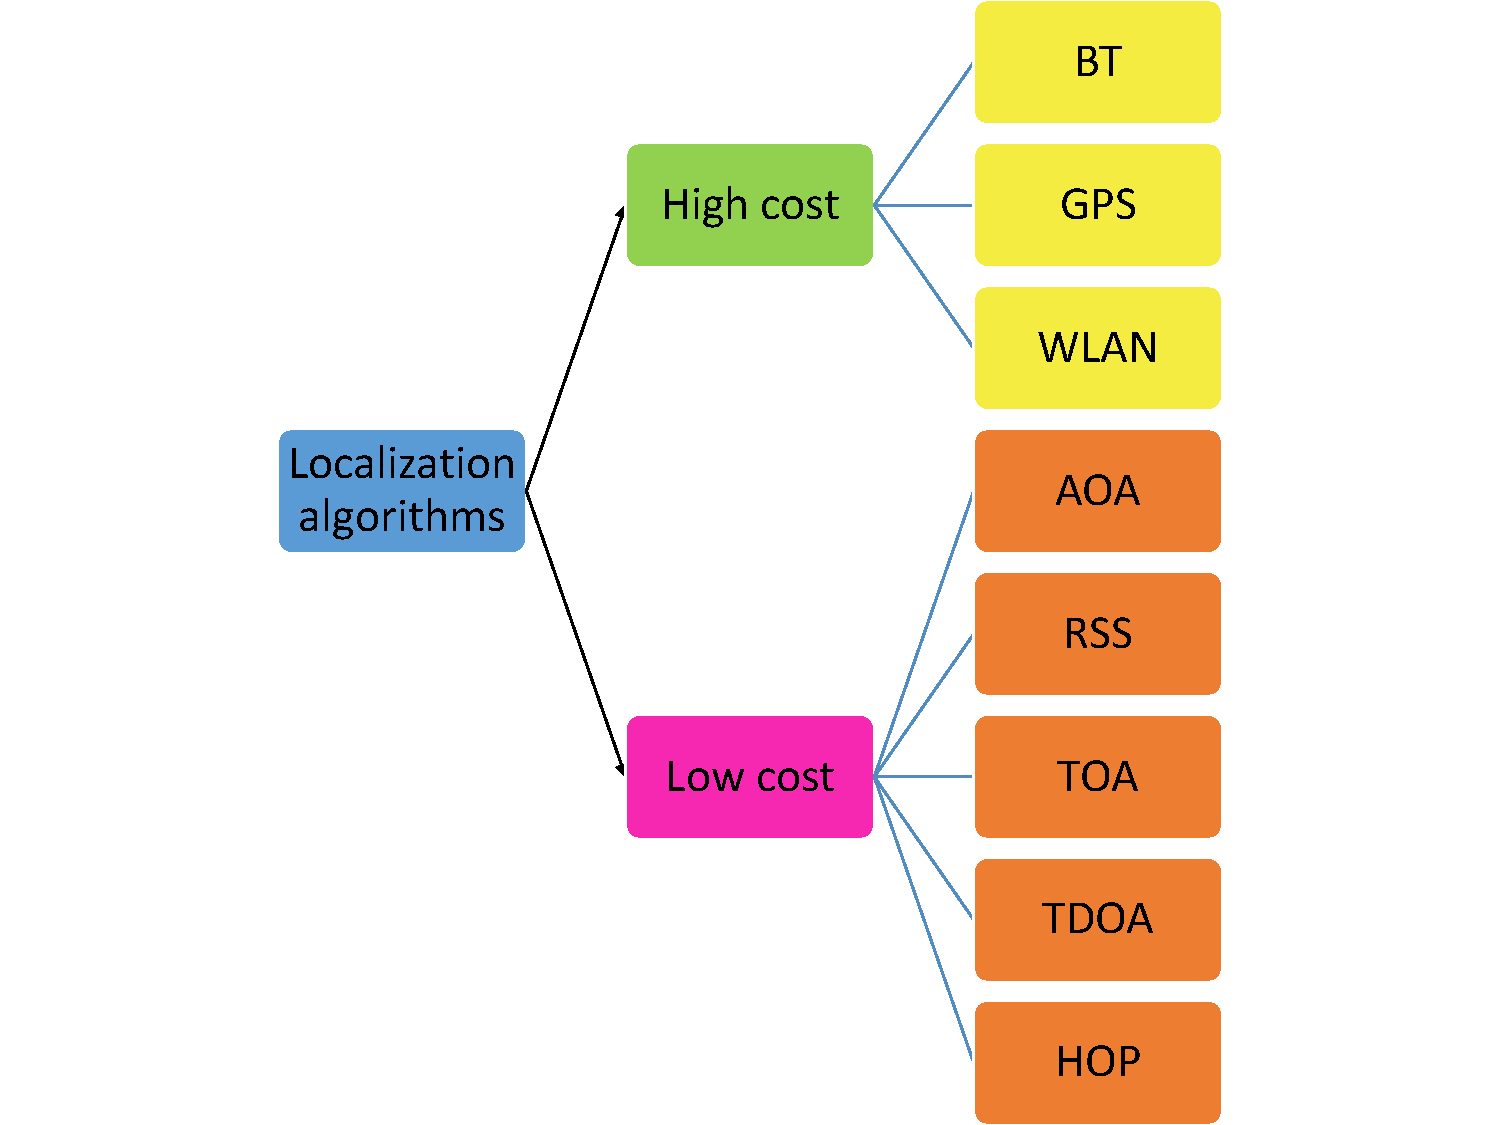
\includegraphics[width=5in]{algs}
\caption{Overview of common localization algorithms}
\label{algs}
\end{figure}

\begin{table}
\renewcommand{\arraystretch}{1.3}
\caption{Summary of common high cost localization techniques.}
\label{hclt}
\centering
\begin{tabular}{L{3cm} L{3.5cm} L{3.5cm} L{3.5cm}}
\toprule
Technique & Overview & Advantages & Disadvantages \\ \midrule
Global Positioning System (GPS) & Location based on satellite tracking of device position & Highly accurate when signal is available & Susceptible to signal blockage and multipath effects \\ 
Wireless Local Area Network (WLAN) & Location based on Wi-Fi signals in a short-range environment & Ideal for indoor environments & Ineffective in long range or outdoor environments \\ 
Bluetooth (BT) & Based on connections between devices & Ideal for small scale node positioning & Even more ineffective than WLAN in long range environments \\ \bottomrule
\end{tabular}
\end{table}

A brief overview of the most common unimodal localization methods of both low cost and high cost categories are presented in Fig.~\ref{algs}. A summary of comparisons among high cost techniques is presented in Table \ref{hclt}.

\subsection{High Cost Localization Methods}

Some of the most common modern localization techniques are well-known even outside of scientific research areas due to their popularities in modern consumer electronics. These localization methods come at a high computational cost but in exchange are more technologically robust and require less mathematical planning. Such techniques include global positioning systems (GPS), wireless local area networks (WLAN), and bluetooth (BT).

GPS is perhaps the most widely known method of localization, whether in a WSN or in a more general navigational context, due to its frequent use in navigational assistance through standalone devices and through embedded navigational capabilities in smartphones and tablet devices. Bluetooth is primarily appealing for short range solutions and thus can be ideal primarily for local positioning in a WSN \cite{shen}. WLAN, or Wi-Fi, is another short range solution whose significance lies within its localization accuracy specific to indoor WSN environments \cite{shen}.

All three of these techniques share the common characteristic of requiring a high computational cost to achieve a desirable level of accuracy. As a result, many scenarios exist in which the desired amount of resources required for proper functionality of GPS, BT, or WLAN are not readily available. In addition, GPS measurements can fall victim to signal blockages or multipath effects \cite{bhatt}. One potential resolution for excessively high cost involves restricting measurement and monitoring capabilities to a small number of nodes known as cluster heads \cite{dhan,desh}, or anchor nodes. A vital further step, however, is to engage in lower cost methods of a more computationally simplistic nature in order to achieve the full potential of effective localization.

\subsection{Low Cost Methods and Terminologies}

\begin{table}
\renewcommand{\arraystretch}{1.3}
\caption{Summary of common low cost localization techniques.}
\label{lclt}
\centering
\begin{tabular}{L{3cm} L{3.5cm} L{3.5cm} L{3.5cm}}
\toprule
Technique & Overview & Advantage & Disadvantage \\ \midrule
Time Difference of Arrival (TDOA) & Time between any two nodes calculated within same frame of time & Better accuracy and performance than TOA in cellular communication systems & Fewer range estimates and increased variance of range sampling error \\ 
Time of Arrival (TOA) & Amount of time required for signal to travel from transmitter to receiver & Only measurement required is time needed to arrive at a node & Can be compromised by undetected direct path conditions and bandwidth limitations \\ 
Angle of Arrival (AOA) & Angle at which signal arrives at receiver from transmitter & Does not require synchronization & Requires expensive antenna arrays at each receiver \\ 
Received Signal Strength (RSS) & Quotient of electric field and distance to some power & Hardware requirements are of low cost & Accuracy can be diminished by environmental factors \\
Hop Count & Number of neighbor nodes required for signal to pass between transmitter and receiver & Range free & Accuracy is compromised when low cost, small size, and high power efficiency are all desired \\ \bottomrule
\end{tabular}
\end{table}

Many established localization techniques exist with a low computational cost compares to the previously discussed methods, but they also require a more significant amount of creativity and mathematical determination. The methods to be discussed in this subsection consist of received signal strength (RSS), angle of arrival (AOA), time of arrival (TOA), time difference of arrival (TDOA), and hop count. A brief comparison of such techniques is presented in Table \ref{lclt}.

\subsubsection{Time Difference of Arrival}

TDOA is a measurement type that determines the time of arrival between two nodes, provided that each pair of nodes uses the same frame of time in such calculations. The main disadvantage of TDOA is the tendency for reduced accuracy from technical constraints in the areas of propagation environments and communication systems \cite{kim}. This is the case when evaluating TDOA on its own. When comparing this measurement type to others, particularly in a specific application, benefits become more prevalent. For instance, in a certain aspect of cellular communication systems, when utilized as localization methods, TDOA holds better performance and higher accuracy than time of arrival (TOA) measurements, although this is at the expense of having fewer range estimates and increased variance of range sampling error \cite{hara}. TDOA is dependent on time differences between nodes \cite{cakir} and thus is another effective means of localization by process of multilateration \cite{pelant}.

\subsubsection{Time of Arrival}

TOA is simply the amount of time required for a signal to move from one transmitter to a receiver \cite{patwari}. This quality diverges from that of TDOA in that only the time needed to arrive at a node is measured, rather than the difference between leaving one node and arriving at another. TOA estimation is known to be more accurate than TDOA in general, rather than in a specific application, although calculating TOA can be more difficult \cite{hwang}. Also worth noting is that the performance of a TOA-based system can be lowered significantly by undetected direct path (UDP) conditions as well as by bandwidth limitations \cite{hatami}. Overall, both time-difference-of-arrival (TDOA) and time-of-arrival (TOA) depend on signal time taken to arrive at the receiver for the source location estimation \cite{yang2,chan}.

\subsubsection{Angle Of Arrival}

\begin{figure}[!t]
\centering
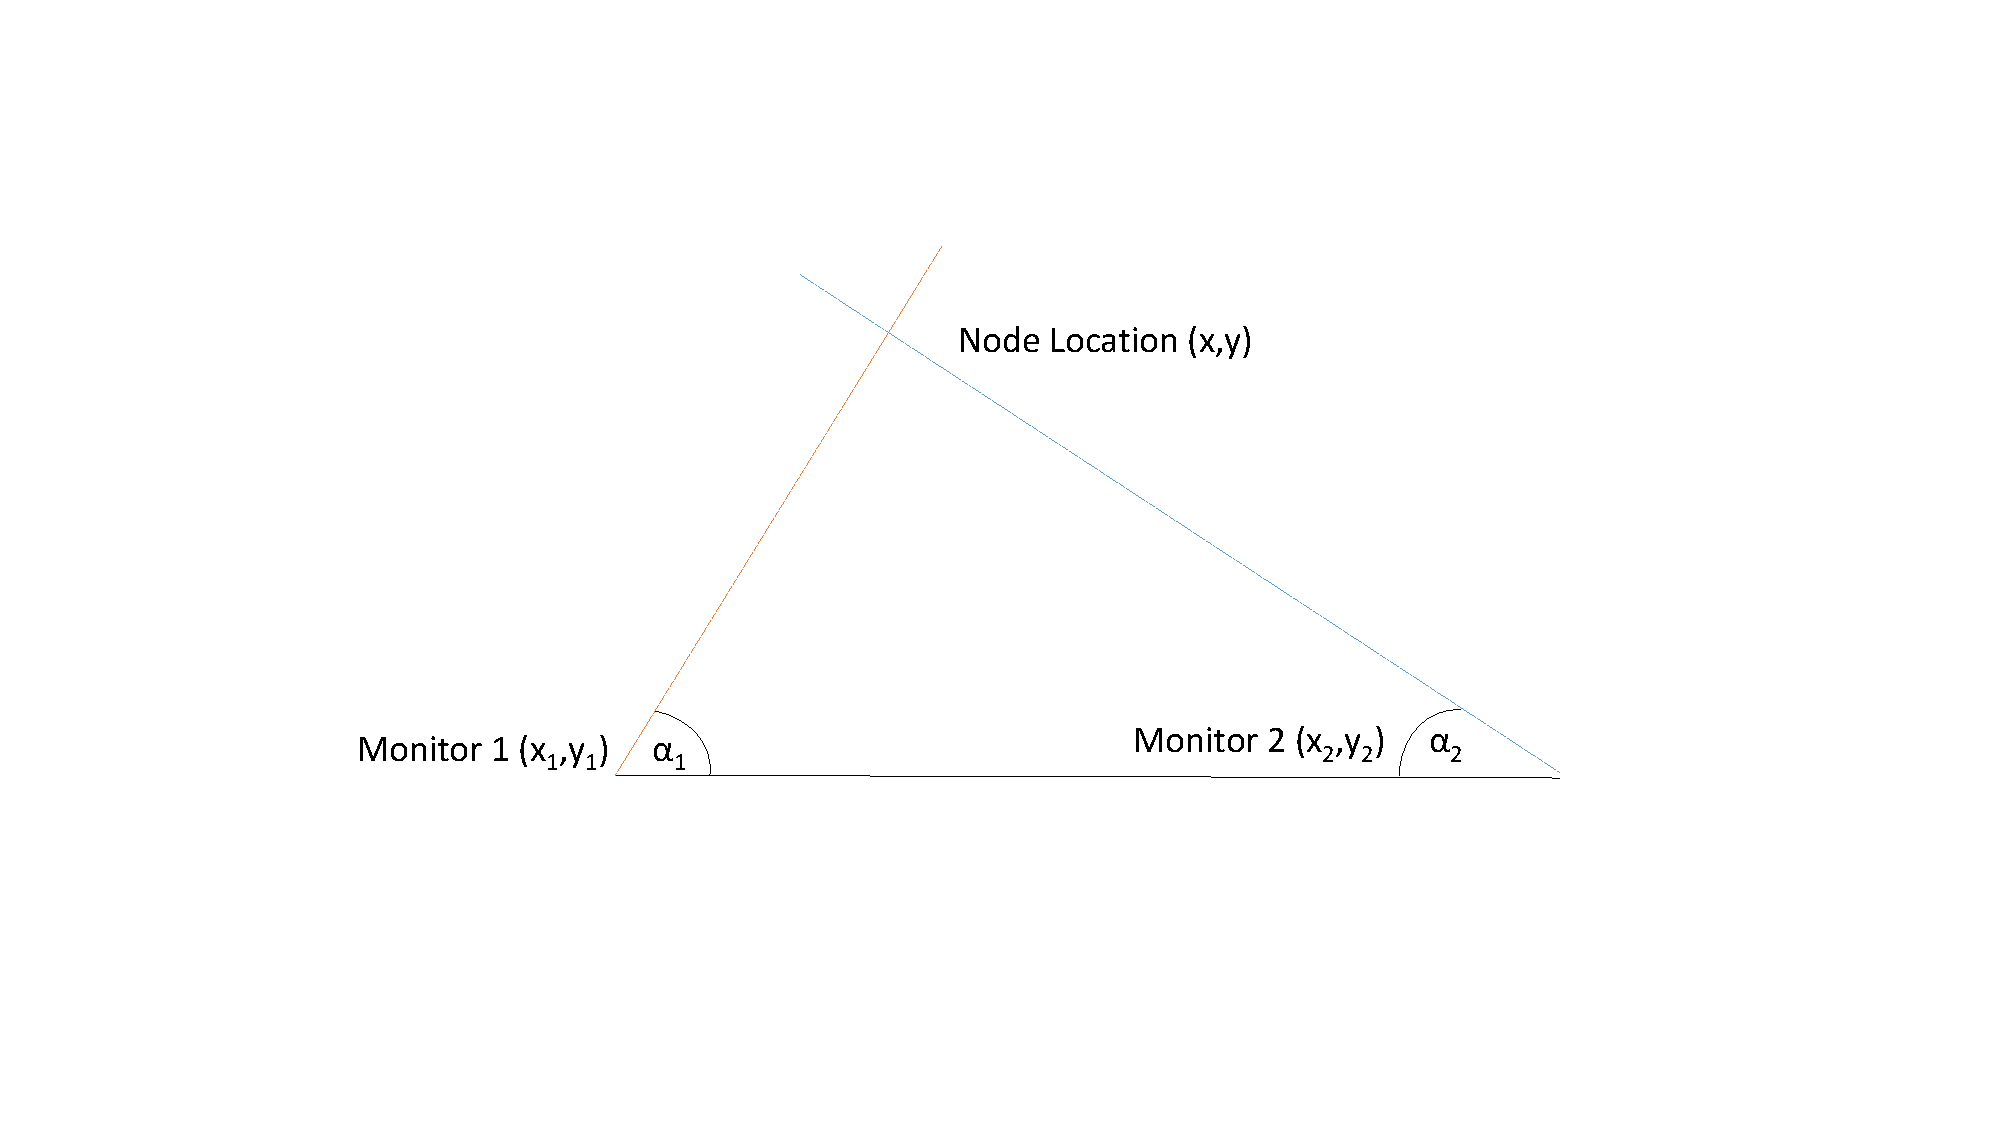
\includegraphics[width=5in]{aoa}
\caption{Example of AOA-based localization}
\label{aoa}
\end{figure}

Angle-of-arrival (AOA) measures the arrival angles at two or more receivers. Location estimation is then done using triangulation \cite{peng,zhang5}. AOA is dependant on the time difference of arrival (TDOA) of multiple elements in an array. TDOA, in turn, is obtained from the difference between phases received by two elements in said array \cite{kumarasiri2}. A practical external example of AOA estimation is the area of smart antenna systems, as the information generated by this type of estimation can be used to enhance the efficiency of transmission and reception of said antenna systems \cite{lee}. In addition, AOA thrives primarily on problems modelled by a Gaussian distribution, particularly in the area of geolocation systems \cite{cheng}. In other words, AOA is the arrival angle of the emitted source signal observed at a monitor (as shown in Fig.~\ref{aoa}) and is a measurement dependent on TDOA of multiple elements in an array. More specifically, AOA is calculated using the differences between arrival times of a transmitted signal \cite{patwari}.

Such localization schemes are of course not without their own disadvantages and limitations. For example, although AOA requires no synchronization and produces satisfactory results with as few as two serving nodes, this measurement type also requires costly antenna arrays at each receiver \cite{kumarasiri2}. Conversely, time of arrival requires at least three receivers for 2-D source locations and generally has better accuracy than AOA schemes. In addition, TDOA and TOA both require synchronization between receivers \cite{kumarasiri2}. In addition, both techniques are highly susceptible to the effects of non-line-of-site (NLOS) conditions \cite{shen}.

\subsubsection{Received Signal Strength}

\begin{figure}[!t]
\centering
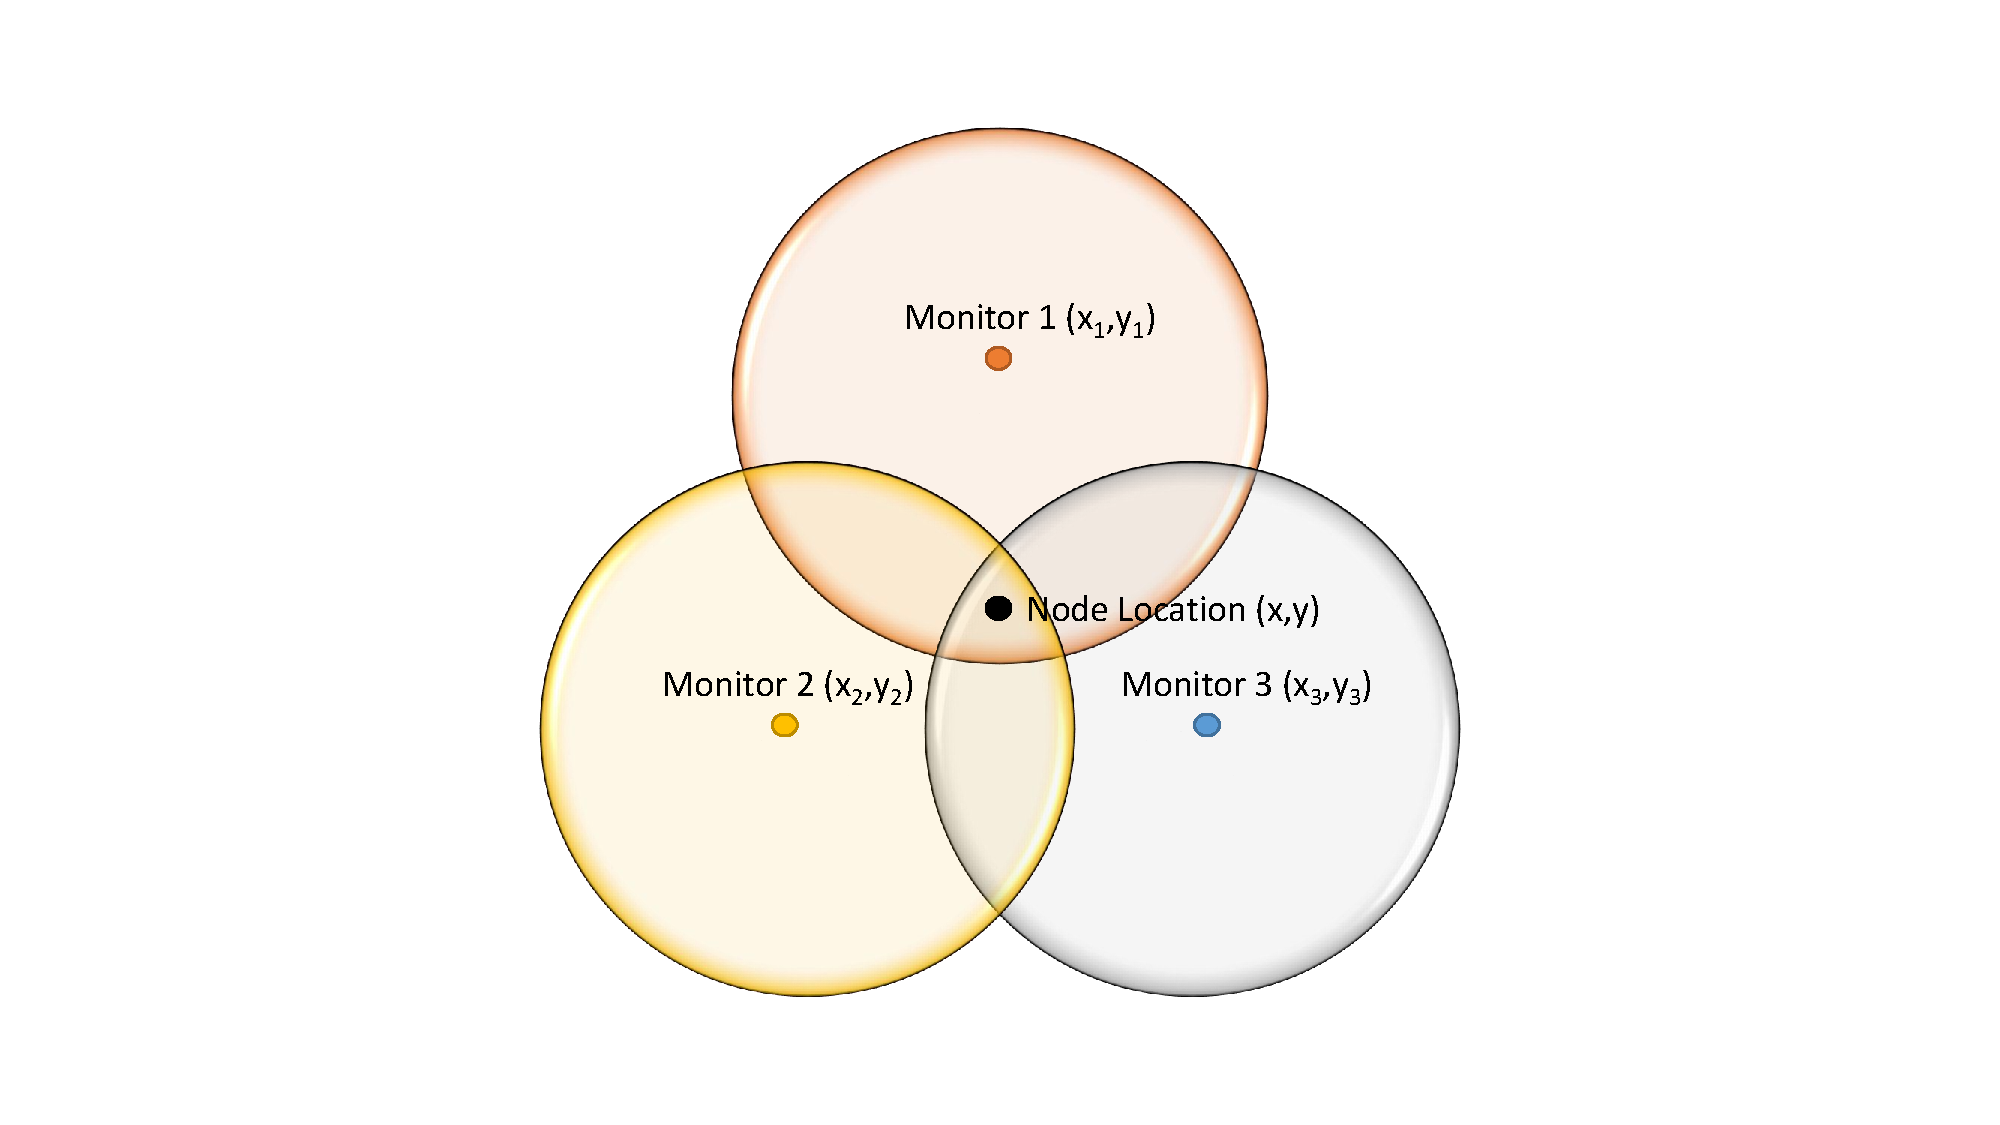
\includegraphics[width=5in]{rss}
\caption{Example of RSS Trilateration in a three-monitor WSN Setup}
\label{rss}
\end{figure}

RSS is the electric field at the receiving node divided by the distance between said node and the transmitter to some power, typically two in free space. The most notable advantage of RSS measurement is that the hardware requirements thereof are inexpensive and simple \cite{dapeng}. The main disadvantage, however, is that RSS accuracy can be compromised by external environmental factors \cite{cheng}. In a more specific context, RSS is the average power received at the anchor node and is given by \cite{song}
\begin{equation}
P_{r}=K\frac{P_{t}}{d^{a}}
\label{rss-eq}
\end{equation}
where $P^t$ is the transmitted power at the source, $d$ is the distance from the source to the receiver, $K$ accounts for all factors that affect the received power, such as antenna heights, and $a$ is the path loss constant. \cite{patwari} defines RSS as the equivalent to measured power, which is the squared magnitude of signal strength. Furthermore, signal power in free space is said to decay proportionally to the square of the distance between a transmitter and receiver \cite{patwari}. \cite{xu} follows a similar approach by defining RSS as the relationship among transmitted power, received power, and distance among nodes in a WSN. This results in the equation
\begin{equation}
P_r=P_t\frac{1}{d^n}
\label{pr-eq}
\end{equation}
where $P_r$ and $P_t$ represent the received and transmitted power, respectively, $d$ denotes the distance between a sending node and a receiving node, and $n$ is a propagation-based transmission factor, which is determined to be two in a free space environment \cite{xu}. Due to RSS's inverse square relationship with distance \cite{xu}, highly accurate locations can be determined with three or more RSS measurements from three unique points by process of trilateration \cite{pivato, so, mazuelas}. An example of trilateration can be seen in Fig.~\ref{rss}. 

\subsubsection{Hop Count}

Hop count is a range-free method that measures the number of intermediate, or neighbor, nodes required for a signal to travel from a sensor node to an anchor node \cite{di} and can be extended into a more refined localization technique using weighted search algorithms \cite{yao}. This method is primarily ideal for networks with low cost, power efficient sensor nodes \cite{beyme}. Range independence is the primary benefit of hop count as a method of localization while the main drawback is that the intended context of low power WSNs typically results in a compromise of accuracy in exchange for low computational cost of the sensor nodes \cite{beyme}.

\subsection{Biologically Inspired Techniques}

\begin{table}
\renewcommand{\arraystretch}{1.3}
\caption{Summary of global, biologically inspired localization techniques.}
\label{global}
\centering
\begin{tabular}{L{3cm} L{3.5cm} L{3.5cm} L{3.5cm}}
\toprule
Technique & Overview & Advantages & Disadvantages \\ \midrule
Genetic Algorithm (GA) & Evolutionary population of candidate solutions & Ideal for large-scale search problems & Premature convergence \\ 
Particle Swarm Optimization (PSO) & Based on particles and movements & Ideal for problems with real values & Expensive computational runtime \\ \bottomrule
\end{tabular}
\end{table}

Table \ref{global} provides an overview of the two most common biologically inspired localization techniques. Genetic algorithms (GAs) are evolutionary algorithms that input a population of potential solutions and converge to a single output candidate \cite{kumarasiri2}. In a process mimicking natural selection, GAs act iteratively, with each iteration evaluating the generation of a population based on the fitness of each candidate solution. These algorithms can be ideal for large scale search-based problems \cite{kumarasiri2}, but they are also disadvantaged by premature convergence \cite{yan,gkou}. Particle swarm optimization (PSO) is also an iterative process that, much like GA, is given a population of possible solutions. Unlike GA's, however,  PSO is based on a convergence of particles, each of which forms movement based upon the most desirable positions available in searchable spaces \cite{kumarasiri2}. The method attempts to improve a solution with respect to a certain level of quality, or termination criteria \cite{luo}. PSO is ideal for optimization scenarios with real values but also possesses the drawback of high computational runtime \cite{ibrahim}, as will be evident in later, result-based portions of this thesis. These global techniques serve as a unique method for WSN localization, either as a standalone technique \cite{gopa} or in combination with other established methods \cite{yang2,ding}.

\subsection{Maximum Likelihood Estimation}

One of such methods that has been included with global optimization is the statistical technique of maximum likelihood estimation (MLE) \cite{ding}, although MLE can also function on its own to achieve robust estimation through utilization of low cost techniques such as RSS \cite{dapeng}. This novel category of estimator searches for the $x$ value that maximizes the likelihood function \cite{nakamura}, defined as
\begin{equation}
\hat{x}(k)=\text{arg max P}(\textbf{z}|x)
\label{mle}
\end{equation}
In the context of WSNs, MLE is most commonly used to estimate distance values to aid in the geolocation of sensor nodes \cite{nakamura}, a strategy that will inspire later developments of this thesis.

\section{Data Fusion} 

Although most of the aforementioned data types, such as RSS and AOA, function well enough on their own, it is when an algorithm can potentially benefit from having multiple types of data that a unique challenge becomes apparent in that each measurement type can be vastly different from one another. To solve this problem of uniquely different data, the concept of data fusion becomes one of vital importance.

Data fusion is a valuable and streamlined process that involves obtaining many different types of data from a single common application and integrating them into a unified, consistent representation, the primary goal of which is to improve the accuracy of a particular algorithm or technique \cite{wang}. In the event of such a large magnitude of complexity within the field of data fusion, a significant amount of creativity and elaboration is needed to solve such a problem. In the context of WSNs, many novel approaches to data fusion have been established, most notably the fusion of RSS and TDOA measurements \cite{hatami}, which in turn can also include the addition of RSS measurements specific to Wi-Fi networks \cite{kumarasiri1}.

\cite{kumarasiri1} proposed the following matrix-based set of equations to determine a measurement vector based on a combination of RSS and TDOA measurements:
\begin{equation}
r = f(\textbf{x}) + n
\label{rk1}
\end{equation}
where
\begin{equation}
\textbf{x}=\begin{bmatrix*}
x \\ y \end{bmatrix*},  r =
\begin{bmatrix*}
r_{rss,1} \\ \vdots \\ r_{rss,N} \\ r_{rss,w,1} \\ \vdots \\ r_{rss,w,M} \\ r_{tdoa,2} \\ \vdots \\ r_{tdoa,N}
\end{bmatrix*}, n = 
\begin{bmatrix*}
n_{rss,1} \\ \vdots \\n_{rss,N} \\ n_{rss,w,1} \\ \vdots \\ n_{rss,w,M} \\ n_{tdoa,2} \\ \vdots \\ n_{tdoa,N}
\end{bmatrix*}, f(\textbf{x}) = 
\begin{bmatrix*}
-a ln(d_1) \\ \vdots \\ -a ln(d_N) \\ -a ln(d_{w,1}) \\ \vdots \\ -a ln(d_{w,M}) \\ d_2 - d_1 \\ \vdots \\ d_N - d_1
\end{bmatrix*}
\label{rk2}
\end{equation}
For Equation \ref{rk1}, $r$ denotes the measurement vector, $f(\textbf{x})$ is a known nonlinear function of the source position $\textbf{x}$, and $n$ is the measurement error vector. In Equation \ref{rk2}, $x$ and $y$ are position coordinates, $M$ and $N$ are the numbers of Wi-Fi-based and non-Wi-Fi-based measurements, respectively, $w$ denotes a Wi-Fi measurement, and $d$ represents distance. Let distance $d_i = d_1,d_2,\dots d_n$ be represented by
\begin{equation}
d_i = \sqrt{(x-x_i)^2+(y-y_i)^2}
\label{dist}
\end{equation}
The use of matrix-based notation becomes particularly useful in later proposed data fusion techniques.

\section{Dempster-Shafer Theory}

Dempster-Shafer (DS) Theory is an innovatively different method of data fusion that can be best summed as a divergence of Bayesian combinational probability, particularly with regards to combinational factors. While Bayesian statistics rely primarily upon combinations of internal probability factors within a system, typically through the use of propositions or random variables, DS Theory is contingent upon external evidence factors, each one consisting of a range of data in which the desired output value can be found as well as a probability of confidence that the data range is in fact reliable. DS Theory is meant to model information that, under more traditional Bayesian methods, would be considered incomplete \cite{nguyen}.

\subsection{Bayesian Origins} 

Bayesian probability is a technique in which two or more internal probabilistic factors are combined to form a single hypothesis or inference, often using random variables to fulfil unknown quantities in the context of a problem \cite{rish}. If only two factors, $X$ and $Y$, are considered, then Bayesian inference can be defined as
\begin{equation}
P(Y|X)=\frac{P(X|Y)P(Y)}{P(X)}
\label{bayes1}
\end{equation}
where $P(X|Y)$ denotes the probability of event $Y$ occurring given event $X$, $P(Y)$ represents the probability of $Y$ alone, $P(x)$ is the probabiliy of $X$ individually, and $P(Y|X)$ is the probability of $X$ given $Y$. 

Bayesian estimation has been established in a variety of applications, including wind speed probability distribution \cite{chiodo1} and battery lifetime analysis \cite{chiodo2}. 

\subsection{Theoretical Foundation}

From a theoretical context, Dempster-Shafer Theory can be best described as a generalization of Bayesian probability theory, forming a divergence based on the concept of ignorance. Typical Bayesian approaches assume an ignorance quantity of zero, or equivalently 100\% confidence, for any probabilistic value, which is usually appropriate when a probability factor is internal. Because DS Theory is based upon external factors, however, this property can no longer be unconditionally assumed, and thus a plethora of evidence factors are used to determine all possible outcomes in a given scenario (e.g. the distance between a sensor node and an anchor node in a WSN), each with its own degree of confidence that serves as a weight of evidence \cite{shafer}. The finite set of all possible mutually exclusive values is known as the frame of discernment and is denoted by $\Theta$. From there, the union of all subsets is given by the power set $2^\Theta$.

\subsubsection{Basic Probability Assignment}

One of the most significant fundamental concepts of DS Theory is the basic probability assignment (BPA) function, which is essentially the equivalent of the random variable in Bayesian probability theory and is also known as the belief variable \cite{auer}, denoted as $m$. Suppose $A_1,\dots,A_n$ are all possible sets within a frame of discernment, noting that $A_i \in 2^\Theta$. Then
\begin{equation}
m: 2^\Theta \rightarrow [0,1], \sum\limits_{i=1}^n m(A_i) = 1, m(\emptyset) = 0
\label{init}
\end{equation}
\noindent where $\emptyset$ denotes the empty set. Each set $A_i$ takes the form of the interval $([\ubar{x},\bar{x}])$, denoting the lower and upper bounds of an evidence factor, respectively \cite{auer}. Each BPA $m$ consists of two vital properties: a range, as established by a set $A$, and a degree of confidence $\mu$ that lies within the range of [0,1] \cite{dempster}. Thus, ignorance can be defined as simply $1 - \mu$. At certain times, manually adding new BPAs can be an exhaustive process, in which case sampling from a distribution becomes an ideal solution. This process, also known as discretization, involves generating $n$ discrete samples based on a lesser amount of initialized BPAs, which collectively form a cumulative density function (CDF) of BPA structures \cite{tonon}.

\subsubsection{Aggregation}

Once two or more evidence factors from different sources exist in the same problem, then typically the aggregation of BPAs becomes essential \cite{auer}. Many possible methods exist in which this task can be accomplished, but the scope of this research focuses primarily upon Dempster's rule of combination. Suppose $m_1$ and $m_2$ denote two BPA functions that are to be aggregated. Under Dempster's rule, a new BPA function $m_1 \oplus m_2 : 2^\Theta \rightarrow [0,1]$ is defined as \cite{al-ani}
\begin{equation}
[m_1 \oplus m_2] = \frac{\sum\nolimits_{A\cap B = y} m_1(A)m_2(B)}{1-\sum\nolimits_{A\cap B = y} m_1(A)m_2(B)}
\label{agg}
\end{equation}
\noindent on the condition that $y \neq 0$. Otherwise $[m_1 \oplus m_2] = 0$. 

\subsubsection{Belief and Plausibility}

Belief and Plausibility are two of the most vital core functions of an aggregate BPA, as they represent the best and worst case scenarios, respectively, in a frame of discernment and are defined as
\begin{equation}
Bel(B) = \sum\nolimits_{A_i \subset B} m(A_i)
\label{bel}
\end{equation}
\begin{equation}
Pl(B) = 1 - \sum\nolimits_{A_i \cap B = \emptyset} m(A_i)
\label{pl}
\end{equation}
\noindent where $m(A_i)$ denotes the BPA mass function for a set $A_i$.

\subsubsection{Prediction of Distance by Expected Value}

In the general area of statistics, expected value is used as a method of predicting the anticipated outcome of an event. Let $x_i$ be a potential outcome in the set of $n$ possible outcomes $x_1,x_2,\dots,x_n$ and let $p_i$ be the probability of $x_i$ occurring. Then the expected value is defined as
\begin{equation}
E(x) = \sum\limits_{i=1}^n x_ip_i
\label{expval}
\end{equation}
\noindent DS Theory contains a similar method of calculating expected value but has a fundamental difference in that the output is a range of values rather than a single value. This is because the lower and upper bounds in a BPA are meant to be addressed separately. Recalling that $\mu$ refers to the degree of confidence, which essentially functions as a probability value, and recognizing the lower and upper bounds of a BPA as $\ubar{x}$ and $\bar{x}$, respectively, the DS expected value is thus defined as \cite{ipp}
\begin{equation}
Val_{Ex} = \sum\nolimits_{BPAs} 
\begin{bmatrix*} \mu \ubar{x} & \mu \bar{x} \end{bmatrix*}
\label{expval}
\end{equation}
\noindent The resultant pair of outputs are then utilized to predict the most likely range of distance between a node's county and a monitor to which the originally given input distance values belong.

\subsection{Applications}

This framework has already been established in a variety of scientific applications, including fault diagnosis \cite{deng}, fault tree analysis \cite{limbourg}, decision analysis \cite{beynon}, text categorization \cite{sarinnapakom}, localization of robot sensors \cite{soleimanpour}, multi-sensor information fusion \cite{yi}, and the fusion of GPS and Inertial Navigational System (INS) data \cite{bhatt}. The general field of WSNs has also explored the potential of DS Theory, such as classification fusion of moving vehicles with a WSN \cite{liu} and network security by means of trust evaluation \cite{feng}. Prior to the validation of this research, however, the use of DS Theory for the specific topic of localization in WSNs has remained widely untapped.

% CHAPTER THREE
      
\chapter{Introductory DS-Based Localization Technique Using Expected Value Outputs of Basic Probability Assignments}

This verbose, introductory technique provides what can be regarded as a hand holding approach to the previously untapped, unexplored terrain that forms when merging Dempster-Shafer Theory with WSN localization. Because the overall goal of this study is to predict an evidence-based location, this method is based on the expected value function of DS Theory and uses basic probability assignments (BPAs) of distance ranges to predict an expected range of radii between a given base station and the potential location of a sensor node. To enhance accuracy, all BPAs are used as distributions for a normalized inverse sample of BPAs, which are then aggregated into a single data structure to be used in all further evaluation. When these radii are obtained for all working monitors, an area of feasible positions is obtained, which can be used to determine whether a particular node in a particular county matches the given set of measurements (RSS, AOA, operating condition, or a combination thereof) corresponding to aforementioned distance BPAs. This approach produces a moderately high range of accuracy, with results ranging from 78-87\%, effectively serving as an adequate start to exploring DS Theory and an easily understandable visual approach to location prediction. A relatively high computational cost, however, leaves this method to be just that, a starter method.

The remainder of this chapter is organized as follows. Section 3.1 compares and contrasts Dempster-Shafer theory with other data modelling techniques. Section 3.2 expands upon the theoretical background of DS Theory established in Section 2.3. Section 3.3 discusses in detail the many facets of the localization algorithm while Section 3.4 explains the experimental parameters and setup. Section 3.5 presents the end results of the experiment as well as a brief discussion of the impact thereof, and lastly, conclusions are drawn in Section 3.6.

\section{Data Modelling} 

Because the overall goal of this research is to effectively predict a node's location in a WSN, Dempster-Shafer Theory can be perceived as a unique type of predictive data modelling. Many methods of predictive data modelling have already been established in the area of WSN localization, such as artificial neural networks (ANNs) and data mining. ANNs are advantageous in their inherent ease of use in simultaneously processing multiple inputs and outputs and modelling highly accurate connection weights thereof using extensive training methods, but they also have their share of drawbacks, as some applications may require significant amounts of training time or fall victim to over-learning and under-learning \cite{almaadeed}. In other words, ANN-based data modelling is ideal for cases in which high accuracy is of greatest importance while high speed and low computational cost are often regarded as lower priorities. 

Data mining tends to follow a reversed trend, in which speed and efficiency are regarded as optimally important even at the cost of  accuracy. In the area of WSN localization, prior established research methods typically utilize data mining with the end goal of fast data collection \cite{patel}. While both methods may appear to be vastly different from one another due to their opposing polarities in the balance of speed and accuracy, each approach holds a vital common characteristic in that they each require dedicated stages for training and validation.

Dempster-Shafer Theory differs greatly from typical data prediction algorithm in two fundamental ways. One is that no training stage is needed to achieve valid and complete results, even when the data to be modelled is in itself considered to be incomplete. The second is that DS Theory contains the potential to achieve results of both high accuracy and low cost, meaning that one attribute can be achieved with no significant reductions in the other.

\section{Dempster-Shafer Theory}

Recall from the literature in Subsubsection 2.3.2.1 that one of the most significant fundamental concepts of DS Theory is the basic probability assignment (BPA) function, which is essentially the equivalent of the random variable in Bayesian probability theory and is also known as the belief variable \cite{auer}, denoted as $m$. Suppose $A_1,\dots,A_n$ are all possible sets within a frame of discernment, noting that $A_i \in 2^\Theta$. Then
\begin{equation}
m: 2^\Theta \rightarrow [0,1], \sum\limits_{i=1}^n m(A_i) = 1, m(\emptyset) = 0
\label{init}
\end{equation}

\noindent where $\emptyset$ denotes the empty set. Also recall that if two or more evidence factors from different sources exist in the same problem, then the BPAs are required to be aggregated \cite{auer}. Under Dempster's rule of combination, suppose $m_1$ and $m_2$ denote two BPA functions that are to be aggregated. Then a new BPA function $m_1 \oplus m_2 : 2^\Theta \rightarrow [0,1]$ is defined as \cite{al-ani}
\begin{equation}
[m_1 \oplus m_2] = \frac{\sum\nolimits_{A\cap B = y} m_1(A)m_2(B)}{1-\sum\nolimits_{A\cap B = y} m_1(A)m_2(B)}
\label{agg}
\end{equation}
on the condition that $y \neq 0$. Otherwise $[m_1 \oplus m_2] = 0$. Resultantly, belief and plausibility can be defined as
\begin{equation}
Bel(B) = \sum\nolimits_{A_i \subset B} m(A_i)
\label{bel1}
\end{equation}
\begin{equation}
Pl(B) = 1 - \sum\nolimits_{A_i \cap B = \emptyset} m(A_i)
\label{pl1}
\end{equation}
where $m(A_i)$ denotes the BPA mass function for a set $A_i$.

\subsection{Linear Representation}

A BPA contains three vital properties: a lower bound $\ubar{x}$, an upper bound $\bar{x}$, and a degree of confidence $\mu$. Hence, a linear representation of a BPA as a vector of these three properties becomes a highly convenient organizational method. In such a case, the resultant BPA $m$ would be defined as 
\begin{equation}
m = \begin{bmatrix*}
\ubar{x} & \bar{x} & \mu \end{bmatrix*}
\label{bpam}
\end{equation}
With such value definitions intact, recall from the end of the literature review that expected value is defined as
\begin{equation}
Val_{Ex} = \sum\nolimits_{BPAs} 
\begin{bmatrix*} \mu \ubar{x} & \mu \bar{x} \end{bmatrix*}
\label{expval}
\end{equation}
In order to effectively represent an aggregate BPA, representation of the individual assignments as a matrix is also beneficial. For this purpose, let $m_1, m_2,\dots,m_n$ represent all BPAs in $\Theta$ such that
\begin{equation}
m = \begin{bmatrix*}
m_1 \\
m_2 \\
\vdots \\
m_n \end{bmatrix*}
= \begin{bmatrix*}
\ubar{x}_1 & \bar{x}_1 & \mu_1 \\
\ubar{x}_2 & \bar{x}_2 & \mu_2 \\
\vdots & \vdots & \vdots \\
\ubar{x}_n & \bar{x}_n & \mu_n \\ \end{bmatrix*}
\label{m}
\end{equation}
Under this method of organization, all BPAs are available for calculation of the expected value range.

\section{Localization Algorithm}

Many aspects of the localization technique are based upon a similar approach proposed in \cite{kumarasiri2}, in terms of selection and measurement of various measurement types, particularly received signal strength (RSS), angle of arrival (AOA), and operating condition (standby). Utilizing the data from said features for the particular process of node positioning, however, follows a significantly different approach, based upon DS expected value, as defined in Subsubsection 2.3.2.4.

\subsection{Measurement Types}

Before RSS, AOA, and operating condition can be mathematically defined, the distance between any sensor node and any anchor node must be evident. Suppose the coordinate $(x_n,y_n)$ refers to the position of a sensor node and $(x_m,y_m)$ is the position of a monitor, or anchor node. Then, the distance $d$ can be defined as 
\begin{equation}
d_{actual} = \sqrt{(x_m^2 - x_n^2) + (y_m^2 - y_n^2)}
\label{dis}
\end{equation}
\noindent where all aforementioned variables are measured in meters. For RSS calculation, many formulae have been established for context-specific calculation, but in the context of free space, all share the property of having an inverse square proportionality with distance. Hence, in the context of this research, RSS is simply defined as the inverse square of distance, or $RSS = 1/d_{actual}^2$. 

Due to the generic nature of this interpretation, no specific unit is needed, as long as the generic unit contains the factor of $m^{-2}$. AOA, however, is defined more strictly as
\begin{equation}
 AOA =
  \begin{cases}
   tan^{-1}(\frac{y_n-y_m}{x_n-x_m}) & \text{if } y_n > y_m \text{ and } x_n > x_m \\
   tan^{-1}(\frac{y_n-y_m}{x_n-x_m}) + 180       & \text{if } y_n \neq y_m \text{ and } x_n < x_m \\
   tan^{-1}(\frac{y_n-y_m}{x_n-x_m}) + 360       & \text{if } y_n < y_m \text{ and } x_n > x_m
  \end{cases}
\label{aoa}
\end{equation}
\noindent with resultant units in degrees. Standby is a unique type of distance measurement in which a sensor node with this feature enabled is detected by a dedicated standby node, which measures the distance thereof by inverse square root RSS calculation. Let $(x_{sb},y_{sb})$ be the location of the standby node. Then the standby distance is defined mathematically as
\begin{equation}
SB = \sqrt{(x_{sb}^2 - x_n^2) + (y_{sb}^2 - y_n^2)}
\label{dis}
\end{equation}
where the subscript $sb$ refers to the $x$ and $y$ coordinates of the standby node.

\begin{figure}[!t]
\centering
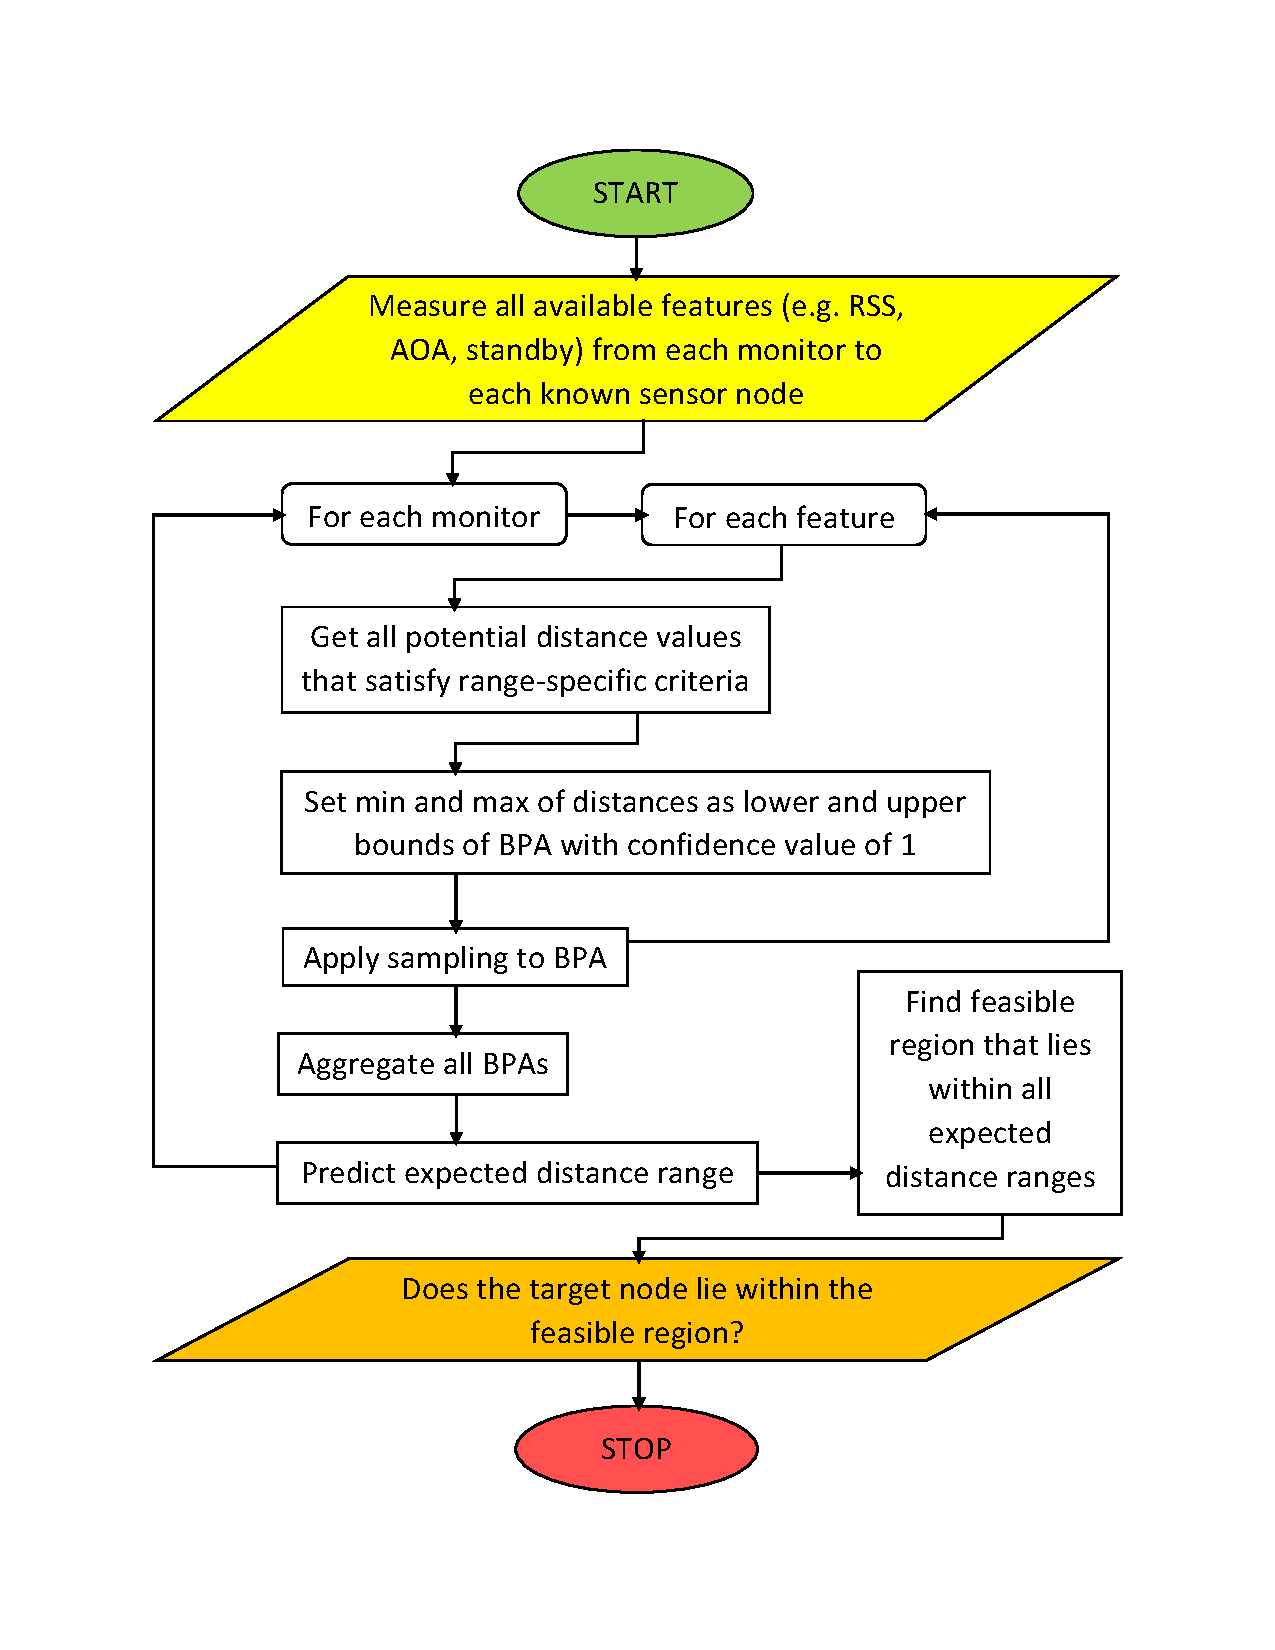
\includegraphics[width=4in]{flowchart1}
\caption{Flowchart of DS localization algorithm.}
\label{dsalg1}
\end{figure}

\subsection{Data Fusion}

In order to fuse any of the varied measurement types (RSS, AOA, standby) together, each measurement must be converted into a common value, which in this case is best represented as the distance from a measurement set to a monitor, as determined by inverse square root RSS calculation. Due to this method of distance determination, the experimental setup will require RSS to be enabled at all times. If a reputable distance or range of distances can be found for all available monitors, then a node's location or respective county can be estimated by an enhanced process of trilateration, in which enhancement is based on the effects of data fusion. The challenge associated with reaching such a goal becomes the task of estimating such a distance range for each monitor. Thus, the need for effective organization and evaluation of optimal distance ranges is where Dempster-Shafer Theory becomes a mechanism of primary interest.

Because external evidence factors are the primary means by which DS-based estimation can occur, the necessity arises to obtain distances and measurement sets that are independent of those given as functional inputs. This distinction will be explained at greater length in Subsection 3.4.2 by means of test data and full data sets. Because such data is external, the amounts and ranges of measurements must be reduced based on feature-specific criteria. Suppose these range values, $r$, are defined as
\begin{equation}
r = \begin{bmatrix*}
r_{RSS} \\
r_{AOA} \\
r_{SB} \end{bmatrix*}
\label{range}
\end{equation}
\noindent where $r_{RSS} > 1$, $0 < r_{AOA} < 1$, and $r_{SB} = -1 $. The latter value indicates that there is no range for standby. If the inverse of a given feature measurement is less than the range $r_i$, the lower and upper limits of such ranges are defined as $|0,1/r_i|$.  Otherwise, if the value is greater than or equal to $r_i$, the limits are $|\frac{s_i}{r_is_i+1},s_i|$, where $s_i$ is the particular feature measurement and $i$ is the gesture type. The next step is to find external distance values from external feature measurements that lie within the corresponding range. Once all of such distance values have been filtered, the minimum and maximum of the remaining values become the respective lower and upper bounds of the resultant BPA. Because all BPAs will aggregate in a later step, the confidence value can simply be 1 for the time being. Thus,
\begin{equation}
m_i = \begin{bmatrix*}
d_{min} & d_{max} & 1 \end{bmatrix*}
\label{bpa-d}
\end{equation}

Once a BPA is formed for each active feature, aggregation can then occur. To smoothen the transition between BPAs however, sampling each $m_i$ by a consistent function handle, such as inverse normalization, is recommended. The resultant aggregate BPA for $n$ samples thus becomes
\begin{equation}
\lambda = \begin{bmatrix*}
\lambda_{RSS} \\
\lambda_{AOA} \\
\lambda_{SB} \end{bmatrix*}
\label{m}
\end{equation}
where
\begin{equation}
\lambda_{RSS} = \begin{bmatrix*}
m_{1,RSS} \\
m_{2,RSS} \\
\vdots \\
m_{n,RSS} \end{bmatrix*},
\lambda_{AOA} = \begin{bmatrix*}
m_{1,AOA} \\
m_{2,AOA} \\
\vdots \\
m_{n,SB} \end{bmatrix*},
\lambda_{SB} = \begin{bmatrix*}
m_{1,SB} \\
m_{2,SB} \\
\vdots \\
m_{n,SB} \end{bmatrix*}
\label{m}
\end{equation}
\noindent This is under the assumption that all three features are enabled. If one or more features are unavailable, then their corresponding $\lambda$ values are simply omitted. In the context of this setup, all confidence values are equal, and hence all $\mu$ values are simply $\frac{1}{3n}$. If fewer than three features are enabled, then $\mu$ is $\frac{1}{fn}$, where $f$ is the number of features. With all aggregation intact, the next step is the actual data prediction process.

\section{Methods and Materials}

A varied plethora of WSN simulation scenarios was created and analysed using the MATLAB scientific programming environment \cite{matlab}. The resultant software package includes all facets needed for experimental simulation, including selectively randomized generation of data, complete implementation of the algorithm proposed in the previous section, and extensive calculation of the algorithm's accuracy.

An overview of the default simulation parameters in the experimental setup is as follows:

\begin{enumerate}
  \item 100 nodes deployed throughout a rectangular region of 1000-by-1000 meters
  \item Three anchor nodes (both options tested separately in identical networks)
  \item Anchor nodes in three-monitor setups located at [150,100], [500,100], and [850,100] meters
  \item Standby node placed at [500,800] meters; location of fusion center is negligible
  \item One-to-one mapping of counties and sensor nodes
  \item Range criteria of 20, 100, and -1 for RSS, AOA, and standby, respectively
  \item Setup tested for RSS+standby, RSS+AOA, and RSS+AOA+standby
  \item Discretization consisting of 10 samples as an inverse normalized distribution
  \item Experimental results as the average of ten independent experiments in which the WSN is regenerated upon every trial
  \item Zero noise factor and zero anchor node positioning error assumed
\end{enumerate}

Details of the variables and terminologies above are explained in the proceeding subsections.

\subsection{WSN Setup}

\begin{figure}[!t]
\centering
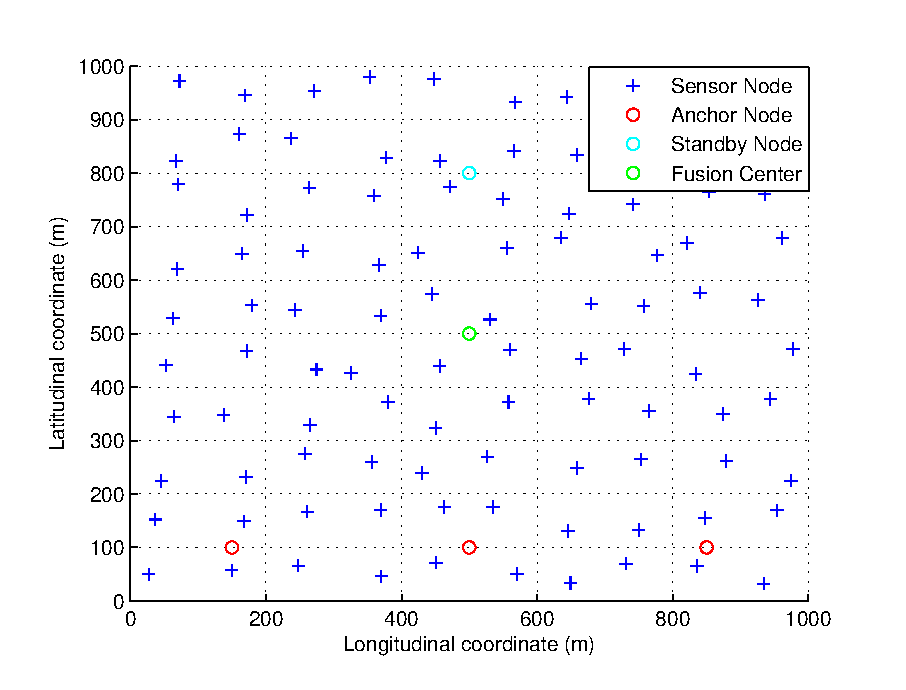
\includegraphics[width=6in]{wsn-plot1}
\caption{WSN of 100 sensor nodes, 3 anchor nodes, standby node, and fusion center.}
\label{wsn}
\end{figure}

The sensor network in this simulation consists of three vital components: the sensor nodes, the anchor nodes, and the fusion center. The sensor nodes comprise the vast majority of the components in this setup, totalling 100 out of 105 nodes in a three-monitor setup. The anchor nodes, also known as monitors or cluster heads, are placed strategically throughout the WSN to measure the available properties of each and every sensor node, such as RSS, AOA, and operating condition (standby), and transmit said data to a fusion center node, which processes all information using the algorithms and methods given in the following subsections. In other words, the fusion center assumes the role of the entire localization software, minus the data generation stage. In addition, a standby node measures the distance of any sensor nodes that are in standby mode. The complete WSN setup is presented in Fig.~\ref{wsn}.

\subsubsection{Data Value Ranges}

In this network setup, the origin of the coordinate system is positioned at the lower left hand corner of the map, as indicated in Fig.~\ref{wsn}. County names and monitor names are given as numbers ranging from one to the total number of counties and monitors available, respectively. All monitors are horizontally aligned by having a common latitudinal coordinate of 100 meters as well as longitudinal coordinates from 150 to 850 meters. Ranges of sensor node coordinates are based on the size of the WSN and can be placed at any location within the region that is more than 30 meters from any border. Based on the criteria of the latter two data types, distances between sensor nodes and monitors can vary from 40 to 1360 meters. RSS, being merely the inverse square root of distance, can range from 1/2000000 to 1/1600.  AOA can be any positive number of degrees up to 360, and the operating condition, or standby distance, can range from 0 to 920 meters.

\subsection{Data Generation}

A multitude of sensor nodes, counties to which each node belongs, and various measurements of nodes relative to various monitors were written to and read from a single comma separated value (CSV) file known as the full data set. Also included in the file are  monitor locations, county locations, and distances from any sensor node to any monitor, calculated from the latter two locations. Each sensor node encompasses multiple rows of data, in which each row corresponds to a particular monitor observing the node and its measurements. Each category of data, such as county number, distance, or a type of measurement, takes the form of a column. The full data set contains one hundred samples of sensor node data for every county in the WSN.

A second CSV file known as the test data set contains the county locations and measurements that are to be tested against the full data set. Although the categories of each column are identical to those of the full data set, the test data contains only one sensor node per county. The location and measurement values of the array are different from any of the nodes of the corresponding county in the full data. In addition, the test data set contains 300 total rows of data while the full data set contains 30,000 rows.

Each sample of data in each file contains ten columns, described as follows:

\begin{enumerate}
	\item Anchor node number
	\item X coordinate of anchor node
	\item Y coordinate of anchor node
	\item County number
	\item County x coordinate
	\item County y coordinate
	\item Distance from county to anchor node
	\item RSS value
	\item AOA value
	\item Standby value
\end{enumerate}

\noindent Worth noting is that the first three values are intended to be treated independently of measurement data in accordance with the algorithm objectives provided in Subsection 3.4.4. In addition, the seventh column is optional to the algorithm, as any distance value can be calculated directly from the corresponding RSS value due to a consistent inverse proportionality between RSS and squared distance.

\subsection{IPP Toolbox}

To aid in the MATLAB implementation of DS Theory, the open source Imprecise Probability Propagation (IPP) Toolbox \cite{ipp} was obtained, released under the GNU General Public License (GPL), and used to execute all DS-specific functions in the simulation, such as formation of BPAs, aggregation and sampling of BPAs, and calculation of expected value, belief, and plausibility.

\subsection{Algorithm Execution}

\begin{algorithm}
\caption{Pseudocode of first proposed DS localization algorithm} \label{alg}
\begin{algorithmic}[1]
\STATE test\_data $\leftarrow$ read measured feature values, county name and location, and monitor locations
\STATE full\_data $\leftarrow$ read potential feature values for the county and monitors
\STATE range $\leftarrow$ feature-specific range values for each active feature
\FORALL{monitors}
	\FORALL{active features}
		\STATE distances $\leftarrow$ all distances corresponding to feature measurements in full\_data that satisfy range
		\STATE BPA\_per\_feat $\leftarrow$ [min\_distance,max\_distance,1]
		\STATE apply sampling to BPA
	\ENDFOR
	\STATE aggregate BPAs
	\STATE [min\_dist, max\_dist] $\leftarrow$ expected value range of BPA
\ENDFOR
\STATE feasible\_points $\leftarrow$ all points that lie within all distance range constraints
\RETURN whether feasible\_points contains county location

\label{dst1}
\end{algorithmic}
\end{algorithm}

\begin{figure}[!t]
\centering
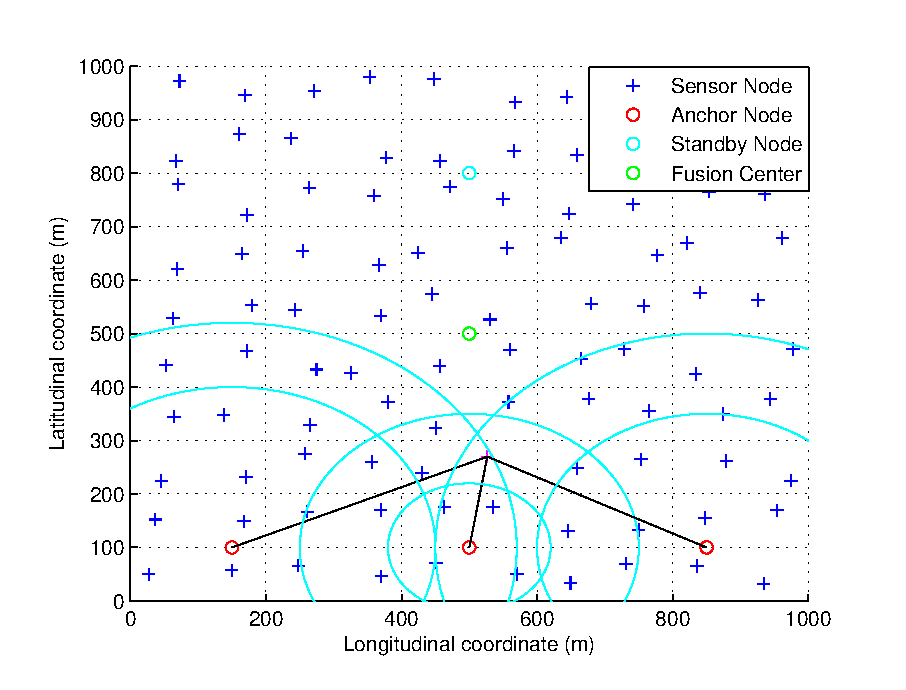
\includegraphics[width=6in]{wsn-plot2}
\caption{Example of expected-value-based DS algorithm in execution.}
\label{demo}
\end{figure}

The algorithm was programmed by following the flowchart provided in Fig.~\ref{dsalg1} and refining the method in the form of the pseudocode provided in Algorithm 1. The pseudocode was then converted into MATLAB-specific syntax and thoroughly tested to ensure proper functionality and accurate representation of the proposed method. A visual example of the technique in action is presented in Fig.~\ref{demo}. The large bright blue circles indicate the expected minimum and maximum radii based on each monitor. The pink plus denotes the node that is being geo-located, while the black lines between said node and each county. Notice how the target node lies within a region that lies within the inner and outer radii for all three monitors.

An important distinction to note is that of the two data files presented in Subsection 3.4.2. In the context of the localization algorithm, the full data set is used only for obtaining distance values for corresponding measurements that fit given range criteria in the distance collection stage, which helps to establish the lower and upper bounds of a BPA. The rest of the algorithm utilizes the test data set, particularly for establishing input values for county locations and measurement sets.

\subsection{Desired Inputs and Output}

\begin{figure}[!t]
\centering
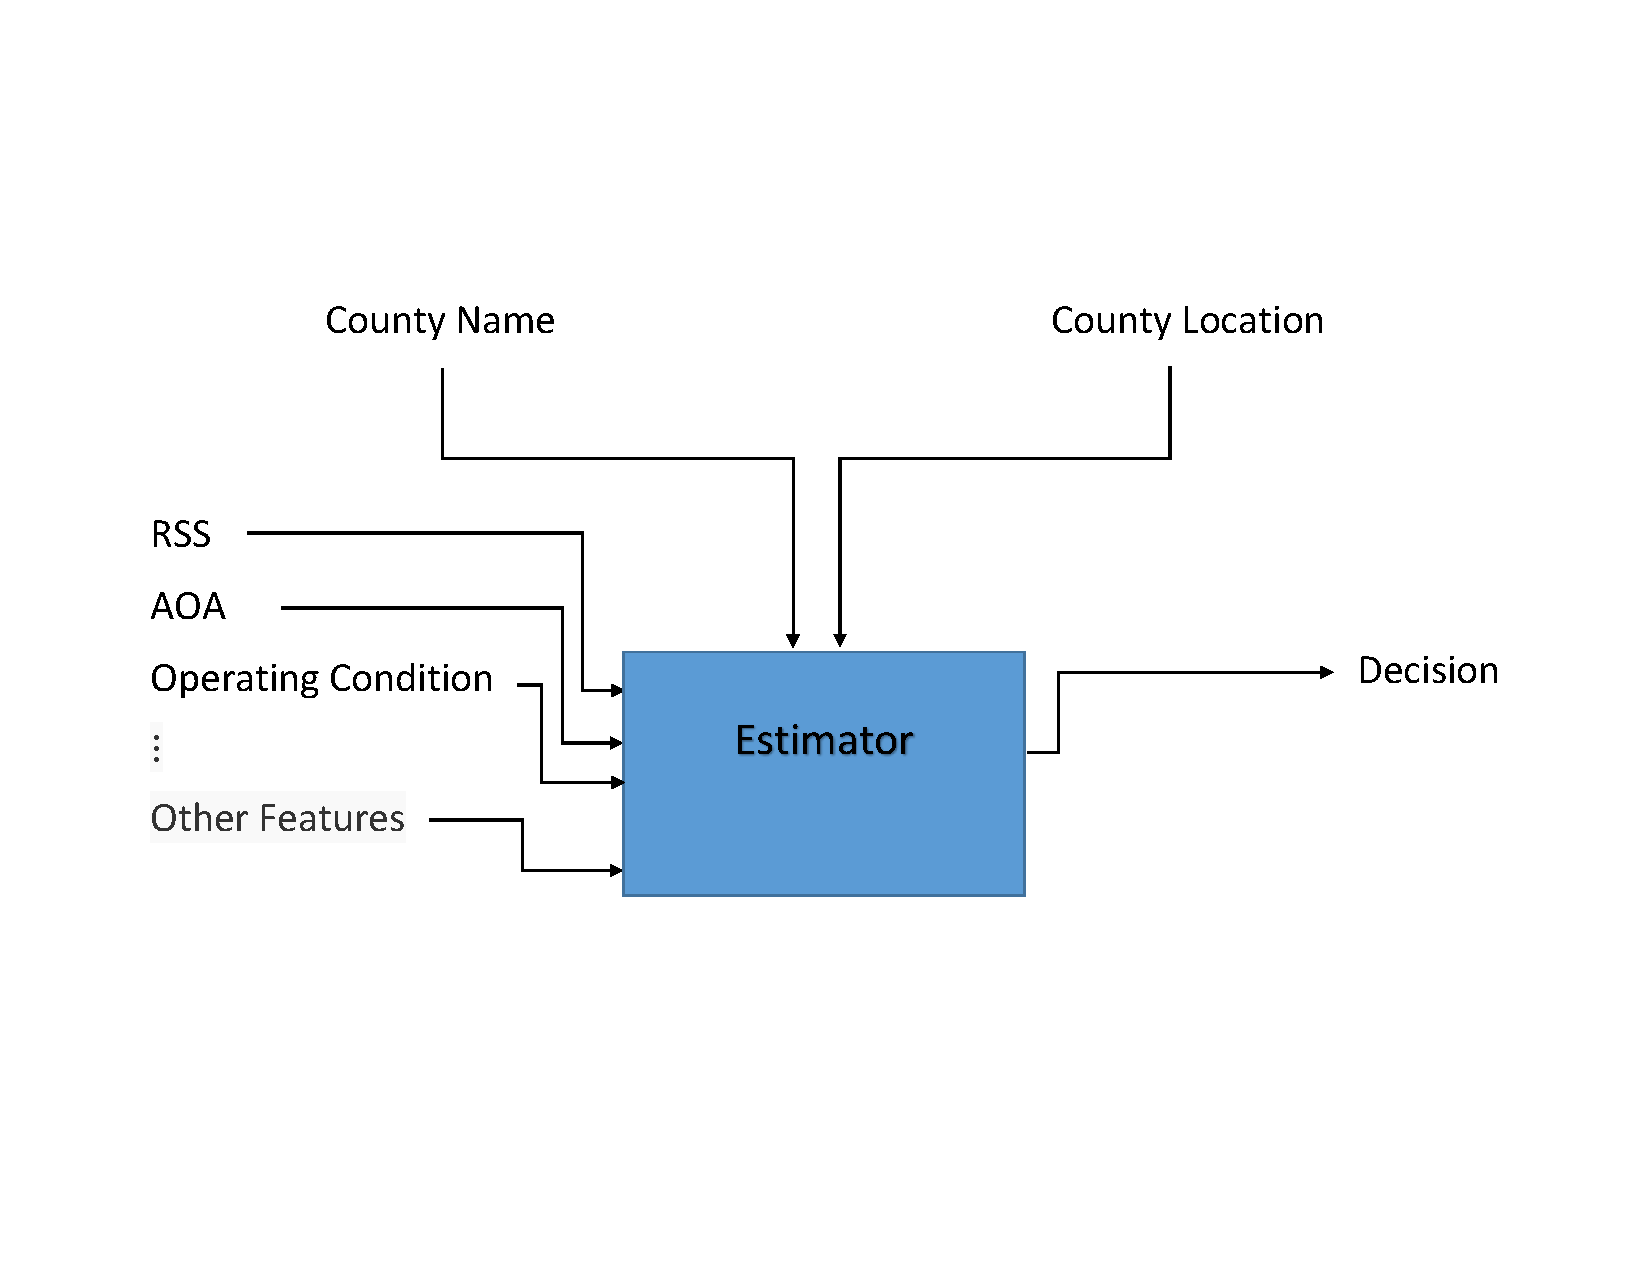
\includegraphics[width=6in]{classifier2}
\caption{First proposed classifier.}
\label{class1}
\end{figure}

A summary of the intended inputs and outputs are given in Fig.~\ref{class1}. This algorithm seeks to answer the following question: given a set of different measurement types and the location of a given county, do the measurements belong to said county?

\subsection{Accuracy Calculation}

\begin{algorithm}
\caption{Pseudocode of DS testing algorithm} \label{alg-test}
\begin{algorithmic}[1]
\STATE test\_data $\leftarrow$ read measured feature values, county name and location, and monitor locations
\STATE full\_data $\leftarrow$ read potential feature values for the county and monitors
\STATE range $\leftarrow$ feature-specific range values for each active feature
\FORALL{measurement sets}
	\FORALL{counties}
		\STATE decision\_per\_county\_per\_mon $\leftarrow$ outputs of Algorithm 1 using test\_data, full\_data, and range as inputs
	\ENDFOR
\ENDFOR
\RETURN decision
	

\label{dst-test1}
\end{algorithmic}
\end{algorithm}

To determine the effectiveness to of the technique presented in the previous subsection, accuracy is calculated as follows. Inputs consist of a single county location and a single list of measurements (as well as their respective distances from a monitor), and a binary decision of one for yes or zero for no serves as the sole output. To test this method of accuracy, every combination of county and measurement set is run through the algorithm as the two inputs, while each output is given in a square matrix whose side length is equal to both the number of counties and the number of measurement sets, where each row corresponds to each measurement set and each column corresponds to each county. This approach is outlined as pseudocode presented in Algorithm 2. Finally, the percent accuracy is calculated by comparing each cell of the resultant matrix against the respective cells an identity matrix of the same dimensions. The resultant formula is as follows:
\begin{equation}
Accuracy = 100*\frac{cells_{matching}}{cells_{total}}
\label{acc}
\end{equation}

\section{Experimental Results}

\begin{table}[!t]
\renewcommand{\arraystretch}{1.3}
\caption{Simulation results.}
\label{table-1}
\centering
$\begin{tabular}{*{3}{l}}
\toprule
Feature Description & Test Accuracy (\%) & Runtime ($\mu$s) \\ \midrule
RSS, SB & 79.97 & 12736.30 \\
RSS, AOA & 78.41 & 12731.71 \\
RSS, AOA, SB & 87.36 & 12731.49 \\ \bottomrule
\end{tabular}$
\end{table}

The number of possible features was determined by addressing the three features (RSS, AOA, operating condition) as a three bit binary combination. Typically, this would result in $2^3=8$ possibilities, but because the algorithm is dependent upon RSS to reverse engineer a measured distance, the RSS bit must always be on, thereby resulting in $2^3-4=4$ possible combinations. In addition, the algorithm proved to be entirely ineffective for single-feature setups, with exactly zero percent accuracy, and hence RSS as a sole feature was omitted from the table, thereby leaving only $2^3-4-1=3$ possible combinations. 

The first column of data in Table \ref{table-1} shows the average accuracy values for all ten generations. As expected, the availability of all three features resulted in the highest accuracy. All trials were run on consistent computer hardware and software, including a standard Windows version of MATLAB on a quad core 2.60 GHz processor and 8.0 GB of RAM. The second column of data in Table \ref{table-1} shows the average runtime results for all ten generations. The significance of these values are addressed in the following subsection.

\subsection{Comparisons to Other Established Algorithms}

To gain further perspective, comparisons were made to four prior established localization methods, including Particle Swarm Optimization (PSO), maximum-likelihood estimation (MLE), a weighted search-based localization algorithm (WSLA), and a weighted search-based refinement algorithm that is combined with the latter technique (referred by \cite{yao} as WSLA+WSRA but reported here as simply WSRA). For the compared methods, the sensor network that was simulated consisted of 100 sensor nodes with eight anchor nodes, and each experiment consisted of 30 independent trials averaged together.

\begin{table}
\renewcommand{\arraystretch}{1.3}
\caption{Comparison of accuracy among different localization techniques.}
\label{compare1}
\centering
$\begin{tabular}{*{6}{l}}
\toprule
Algorithm & PSO & WSLA & WSRA & MLE & DS1 \\
\midrule
Accuracy (\%) & 71 & 90 & 92 & 93 & 87 \\
Runtime ($\mu$s) & 114570 & 7800 & 9700 & NR & 12733 \\
\bottomrule
\end{tabular}$
\end{table}

\subsubsection{Accuracy}

The results are based on those presented in \cite{yao} under the assumptions of no positioning error on anchor nodes and no noise factor. The accuracy values were determined by reported error values under aforementioned conditions, which were then subtracted from one and converted to a percentage. Because error values were reported as a plot rather than in exact numerical form, estimation based on eyeing and measuring the graphs was required to obtain error values; hence, to minimize any potential reporting error, accuracy of each algorithm was reported as a whole number percentage. For the proposed technique (labelled as DS1), accuracy was determined by averaging results for all four feature combinations, rounded to the nearest whole number percentage for consistency. The first row of data in Table \ref{compare1} shows all reported accuracies.

\subsubsection{Computational Runtime}

Average runtime per node for a three-monitor WSN setup was compared with three of the four aforementioned techniques, based on data given in \cite{yao}. The competing data was provided in a table of average CPU time per node with no anchor node positioning error and no noise factor. Hardware specifications and MLE runtime were not reported. All method runtimes, sans that of MLE (which is therefore listed as NR, or not reported), are reported in the second row of data in Table \ref{compare1}. Results for both accuracy and runtime indicate that the proposed method contains significant advantages over PSO but still pale in comparison to the other reported methods.

\section{Conclusions and Future Work}

This chapter presented a new approach to wireless sensor network localization through incorporation of Dempster-Shafer Evidence Theory and the use of its expected value function. This new approach serves as an adequate start to exploring DS Theory by providing a moderately high accuracy and an easily understandable visual approach to location prediction, but a modest accuracy and a high computational cost leaves this method to be just that, a starter method. Luckily, the following approach presented in the next chapter addresses and resolves all shortcomings incurred by this method at the slight expense of less verbosity.

% CHAPTER FOUR

\chapter{Low Cost, Highly Accurate DS-Based Method of Localization Using Plausibility}

While the expected value function provided an adequate, introductory approach to WSN localization within the realms of Dempster-Shafer Theory, many other DS functions served as potential contenders to drive the core of the localization technique. Upon preliminary testing of other functions and their outputs' correlations with measured distances, the concept of plausibility was proven to be the most effective function in terms of both high accuracy and low cost. Leaving most other components of the algorithm to be the same as in the previous chapter, a rigorous set of testing determined this new method to be up to 98\% accurate in a fraction of the time required for mere completion of the previous technique.

The remainder of this chapter is organized as follows. Section 4.1 expands upon the theoretical background of DS Theory established in Section 3.2 as well as an overview of the revised algorithm. Section 4.2 briefly discusses the differences in the localization algorithm from that of the previous chapter. Section 4.3 provides an overview of how the research study was conducted, emphasizing both the similarities to and differences from the experimental setup in Section 3.3. Section 4.4 presents the end results of the experiment in a variety of scenarios as well as a brief discussion of the impact thereof, and lastly, conclusions are drawn in Section 4.5.

\section{Dempster-Shafer Theory}

Recall from the previous chapter that
\begin{equation}
m = \begin{bmatrix*}
m_1^u \\
m_2^u \\
\vdots \\
m_n^u \end{bmatrix*}
= \begin{bmatrix*}
\ubar{x}_1^u & \bar{x}_1^u & \mu_1^u \\
\ubar{x}_2^u & \bar{x}_2^u & \mu_2^u \\
\vdots & \vdots & \vdots \\
\ubar{x}_n^u & \bar{x}_n^u & \mu_n^u \\ \end{bmatrix*}
\label{m-1}
\end{equation}
\noindent The addition of the superscript $u$ now indicates that $\bar{x}_1^u < \bar{x}_2^u < \dots < \bar{x}_n^u$. This is of particular importance, as this sorted order of upper bounds can be used to define belief from a more specific, matrix-oriented context. From here, belief can be represented as
\begin{equation}
Bel = \begin{bmatrix*}
\bar{x}_1^u & \mu_{1,new}^u \\
\bar{x}_2^u & \mu_{2,new}^u \\
\bar{x}_3^u & \mu_{3,new}^u \\
\vdots & \vdots \\
\bar{x}_n^u & \mu_{n,new}^u \end{bmatrix*}
\label{m}
\end{equation}
where 
\begin{equation}
\mu_{1,new}^u = \mu_1^u
\label{mu1l}
\end{equation}
\begin{equation}
\mu_{2,new}^u = \mu_2^l+\mu_{1,new}^u
\label{mu2l}
\end{equation}
\begin{equation}
\mu_{3,new}^u = \mu_3^u+\mu_{2,new}^u
\label{mu3l}
\end{equation}
\noindent and
\begin{equation}
\mu_{n,new}^u = \mu_n^u+\mu_{(n-1),new}^u
\label{munl}
\end{equation}
\noindent Now suppose $m$ is rearranged and $m_{1}^{u}, m_{2}^{u},\dots, m_{n}^{u}$ are renamed such that 
\begin{equation}
m = \begin{bmatrix*}
m_1^l \\
m_2^l \\
\vdots \\
m_n^l \end{bmatrix*}
= \begin{bmatrix*}
\ubar{x}_1^l & \bar{x}_1^l & \mu_1^l \\
\ubar{x}_2^l & \bar{x}_2^l & \mu_2^l \\
\vdots & \vdots & \vdots \\
\ubar{x}_n^l & \bar{x}_n^l & \mu_n^l \\ \end{bmatrix*}
\label{mu}
\end{equation}
\noindent where $\ubar{x}_{1}^{l} < \ubar{x}_{2}^{l} < \dots < \ubar{x}_{n}^{l}$ and the superscript $l$ indicates that contents of $m$ are now arranged in order of increasing lower bound. Hence, all conditions are available to define plausibility as
\begin{equation}
Pl = \begin{bmatrix*}
\ubar{x}_1^l & \mu_{1,new}^l \\
\ubar{x}_2^l & \mu_{2,new}^l \\
\ubar{x}_3^l & \mu_{3,new}^l \\
\vdots & \vdots \\
\ubar{x}_n^l & \mu_{n,new}^l \end{bmatrix*}
\label{m}
\end{equation}
\noindent where
\begin{equation}
\mu_{1,new}^l = \mu_1^l
\label{mu1u}
\end{equation}
\begin{equation}
\mu_{2,new}^l = \mu_2^l+\mu_{1,new}^l
\label{mu2u}
\end{equation}
\begin{equation}
\mu_{3,new}^l = \mu_3^l+\mu_{2,new}^l
\label{mu3u}
\end{equation}
\noindent and
\begin{equation}
\mu_{n,new}^l = \mu_n^l+\mu_{(n-1),new}^l
\label{munu}
\end{equation}

In other words, the top and bottom rows of the belief matrix represent the least and most believable outcomes, respectively. The latter is the row of greatest importance, where $\bar{x}_n^u$ is the value of the most believable outcome and $\mu_{n,new}^u$ is the belief probability, which in this case is always 100\% or one since it is the sum of all confidence values. Similarly, the top and bottom rows of the belief matrix respectively represent the least and most plausible outcomes. Also likewise to belief, the most believable row is of most significance, as $\ubar{x}_n^l$ signifies the most plausible outcome and $\mu_{n,new}^l$ is another 100\% probability. Due to these powerful methods of outcome prediction, development of the proposed localization technique is based extensively on the experimental exploration of these two functions.

\section{Localization Algorithm}

\begin{figure}[!t]
\centering
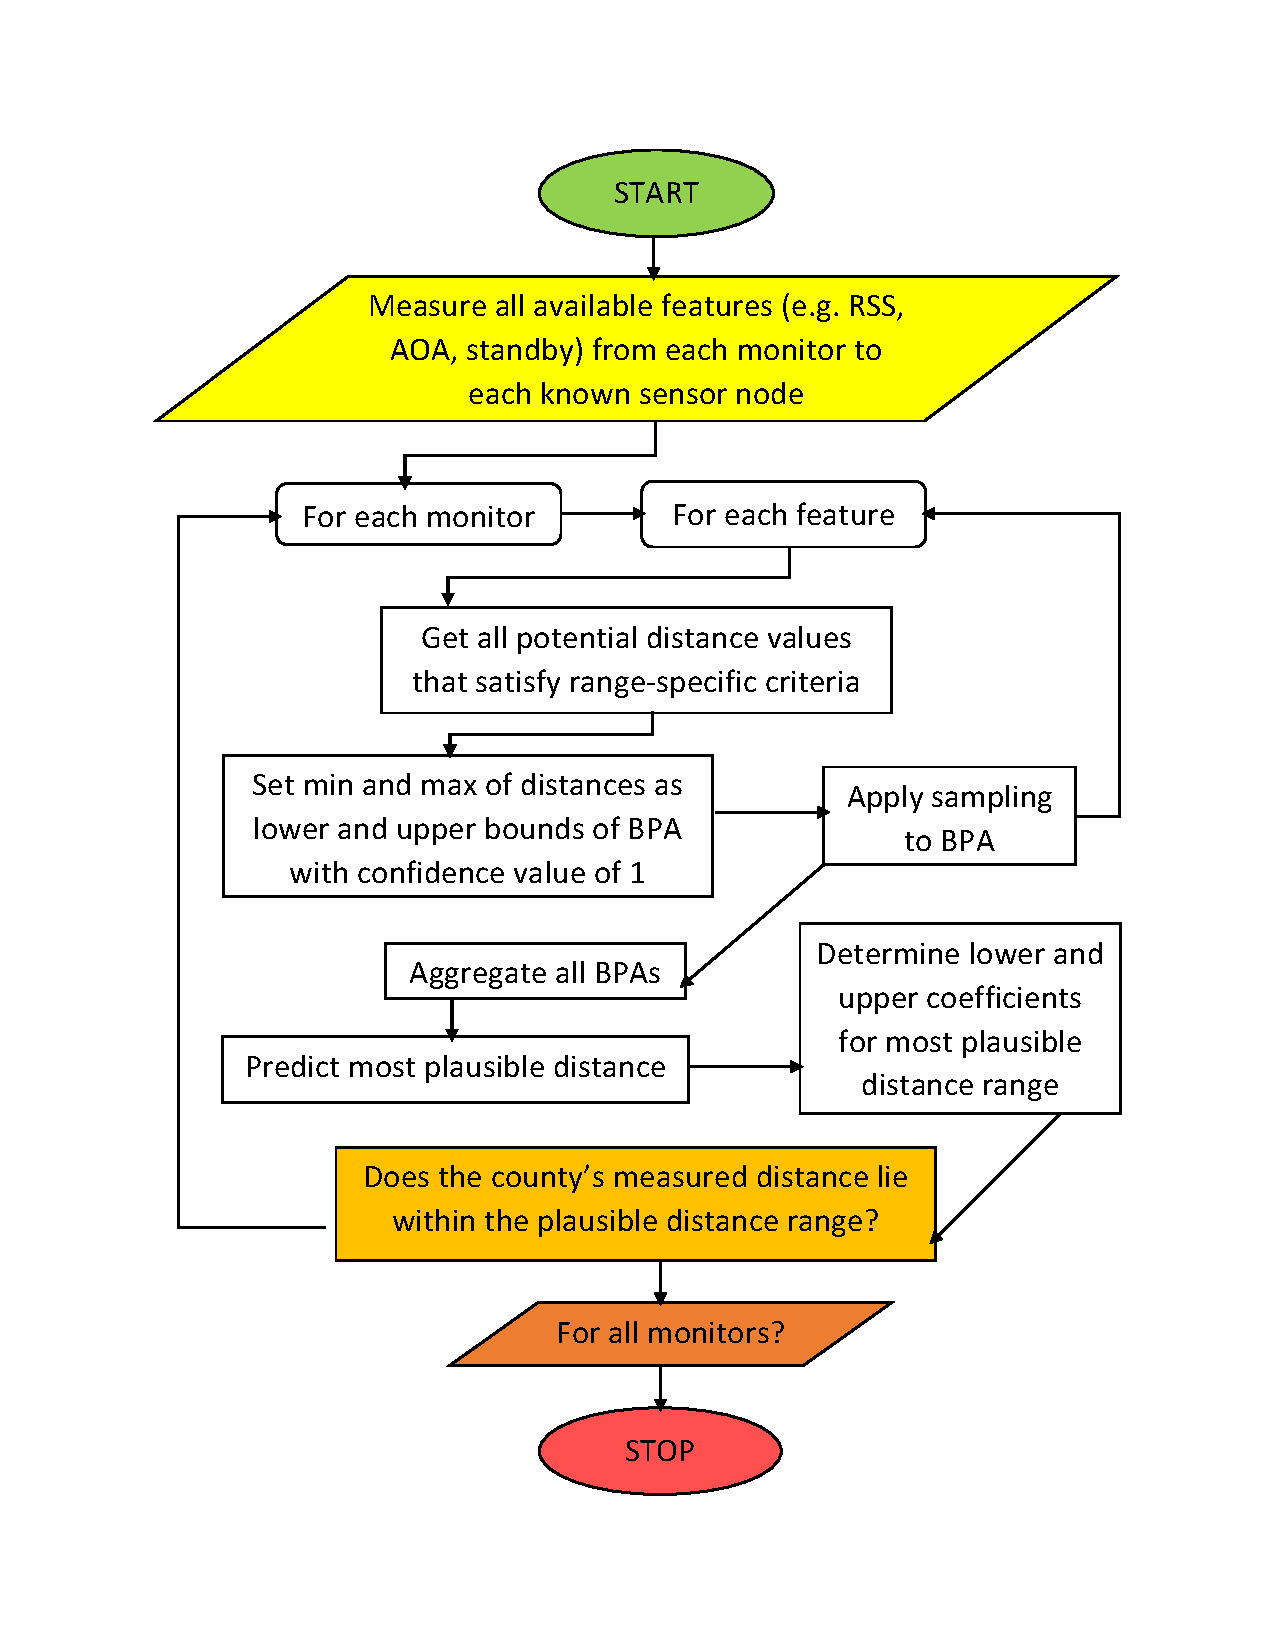
\includegraphics[width=4in]{flowchart2}
\caption{Flowchart of DS localization algorithm}
\label{dsalg2}
\end{figure}

The localization algorithm works mostly in the same way as that of the previous chapter but with expected value replaced with plausibility. Because Dempster-Shafer Theory is an entirely new concept in the area of WSN localization, a clear relation between measured distance and believed or plausible distance was not available in any found literature. Thus, preliminary experimentation was needed to understand how $Bel$ and $Pl$ functions could potentially correlate measured values with calculated values. The resultant analysis from belief and plausibility calculations showed that the former method contained little to no effect in predicting a given distance while the latter showed encouragingly high correlation. Hence, the localization algorithm becomes complete and is presented in Fig.~\ref{dsalg2}.

\section{Material and Methods}

%\begin{figure}[!t]
%\centering
%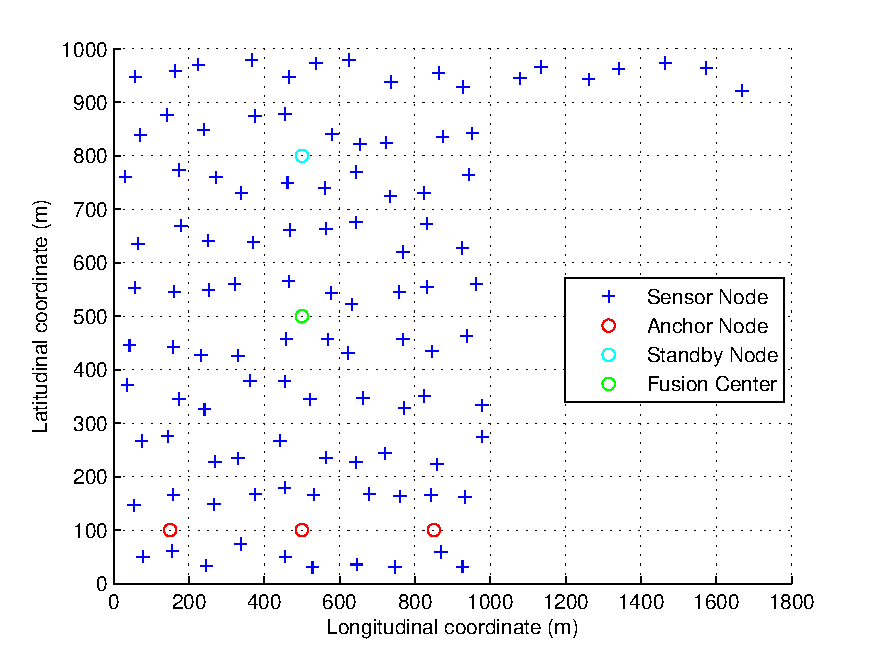
\includegraphics[width=6in]{wsn}
%\caption{WSN of 107 sensor nodes, 3 anchor nodes, standby node, and fusion center.}
%\label{wsn3}
%\end{figure}

An overview of the default parameters in the experimental setup is as follows:

\begin{enumerate}
  \item 100 nodes deployed throughout a rectangular region of 1000-by-1000 meters
  \item Two or three anchor nodes (each option tested separately in identical networks)
  \item Anchor nodes in both two-monitor and three-monitor setups located at [150,100] and [850,100] meters; third anchor node in three-monitor setups located at [500,100] meters
  \item Standby node placed at [500,800] meters; location of fusion center is negligible
  \item One-to-one mapping of counties and sensor nodes
  \item Range criteria of 20, 0.002, and -1 for RSS, AOA, and standby, respectively
  \item Setup tested for every combination of features in which RSS is active (as RSS is needed to calculate distance from node to monitor)
  \item Discretization consisting of 10 samples as an inverse normalized distribution
  \item Differences of -1.5 meters or less for actual distance minus predicted distance disregarded in determining a minimum difference between distances
  \item Distance range weights determined through iterative training (see Subsubsection 4.2.1.1) to be 1.3 and 0.95
  \item Experimental results as the average of ten independent experiments in which the WSN is regenerated upon every trial
  \item Zero noise factor and zero anchor node positioning error assumed
\end{enumerate}

Details of the variables and terminologies above that differ from those given in the previous chapter are explained in the proceeding subsections.

\subsection{Algorithm Execution}

\begin{algorithm}
\caption{Pseudocode of second proposed DS localization algorithm.} \label{alg}
\begin{algorithmic}[1]
\STATE test\_data $\leftarrow$ read measured feature values, county name and location, and monitor locations
\STATE full\_data $\leftarrow$ read potential feature values for the county and monitors
\STATE range $\leftarrow$ feature-specific range values for each active feature
\FORALL{monitors}
	\FORALL{active features}
		\STATE distances $\leftarrow$ all distances corresponding to feature measurements in full\_data that satisfy range
		\STATE BPA\_per\_feat $\leftarrow$ [min\_distance,max\_distance,1]
		\STATE apply sampling to BPA-
	\ENDFOR
	\STATE aggregate BPAs
	\STATE pl\_dist $\leftarrow$ most plausible distance value
	\STATE meas\_dist $\leftarrow$ measured distance from county to monitor
	\STATE [min\_accept, max\_accept] $\leftarrow$ coefficients of acceptable dist values
	\STATE decision\_per\_mon $\leftarrow$ min\_accept < meas\_dist < max\_accept
	\STATE difference\_per\_mon $\leftarrow$ meas\_dist - pl\_dist
\ENDFOR
\IF{decision\_per\_mon == all ones}
	\STATE decision $\leftarrow$ 1
\ELSE
	\STATE decision $\leftarrow$ 0
\ENDIF
\STATE difference $\leftarrow$ minimum difference\_per\_mon
\RETURN [decision, difference]

\label{dst}
\end{algorithmic}
\end{algorithm}

The algorithm was coded by following the flowchart provided in Figure \ref{dsalg2}, which evolved into the pseudocode provided in Algorithm 3, which was then revised to MATLAB-specific syntax and thoroughly tested to ensure proper functionality and accurate representation of the proposed method.

\subsubsection{Determination of Acceptable Distance Values}

As stated in Line 13 of Algorithm 3, a major factor in determining the desired outputs in the next subsection is the formation of acceptable distance values. One of the fundamental strengths of DS Theory is the ability to forego an elaborate training stage that is required in neural network and data mining techniques. Conversely, however, care must be taken to determine a precise distance range to ensure optimal localization accuracy; hence, a simple iterative approach is taken to find the most effective weights for the lower and upper bounds of an acceptable distance range. The resultant approach is detailed in Algorithm 4. For the sake of preserving the training-independent property of DS Theory, and due to the highly intensive time requirement when compared to Algorithm 3, this method is not intended to be executed upon every run of the core algorithm but instead is only to be run upon the initial formation of the WSN as well as highly significant changes thereof. In other words, if a WSN undergoes minor changes, such as the addition or removal of one anchor node or the relocation of sensor nodes across short distances, the impact of the acceptable distance ranges is too low to noticeably alter the accuracy of the core algorithm. The three types of accuracy portrayed in Algorithm 4 as well as the details of Algorithm 5 are provided in Subsection 4.3.3.

\begin{algorithm}
\caption{Pseudocode of distance range training algorithm.} \label{alg-train}
\renewcommand{\arraystretch}{1.3}
\begin{algorithmic}[1]
\STATE test\_data $\leftarrow$ read measured feature values, county name and location, and monitor locations
\STATE full\_data $\leftarrow$ read potential feature values for the county and monitors
\FORALL{candidate upper bounds}
	\FORALL{candidate lower bounds}
		\FORALL{combinations of available features}
			\STATE generate WSN data and run Algorithm 5 set number of times using corresponding bounds and feature set as inputs
			\STATE [decision\_matrix, matching\_county\_vector] $\leftarrow$ average outputs of Algorithm 5
			\STATE [longAcc, shortAcc, matchAcc] $\leftarrow$ long accuracy, short accuracy, and matching accuracy, respectively
		\ENDFOR
		\STATE avgAcc $\leftarrow$ $\frac{1}{3}$ $\frac{1}{no. feat.}$ $\sum\nolimits_{features}$($longAcc$ + $shortAcc$ + $matchAcc$)
	\ENDFOR
\ENDFOR
\STATE  bestAcc $\leftarrow$ maximum avgAcc
\STATE [best\_lower, best\_upper] $\leftarrow$ combination of upper and lower bounds that result in bestAcc
\FORALL{combinations of available features}
	\STATE generate WSN data and evaluate Algorithm 5 using best\_lower, best\_upper, and corresponding feature set
\ENDFOR

\label{dst}
\end{algorithmic}
\end{algorithm}

In typical training techniques for data modelling, the data used for training is intended to contain several times as many samples as those used in validation. Hence, in this approach, WSN data generation and Algorithm 5 execution are run repeatedly and independently three times as much as they are run in the validation and training-independent stages. Due to the high computational time and cost required for training, only a limited number of weight combinations are considered. In this case, the candidate upper weight choices range from 1.1 to 1.9 in increments of 0.2 while the lower weight choices vary from 0.2 to 0.95 in increments of 0.25. As will be indicated in Subsection 4.4.1, the resultant lower and upper bound coefficients of the maximum plausibility value are ultimately chosen to be 1.3 and 0.95, respectively.

\subsection{Desired Outputs}

\begin{figure}[!t]
\centering
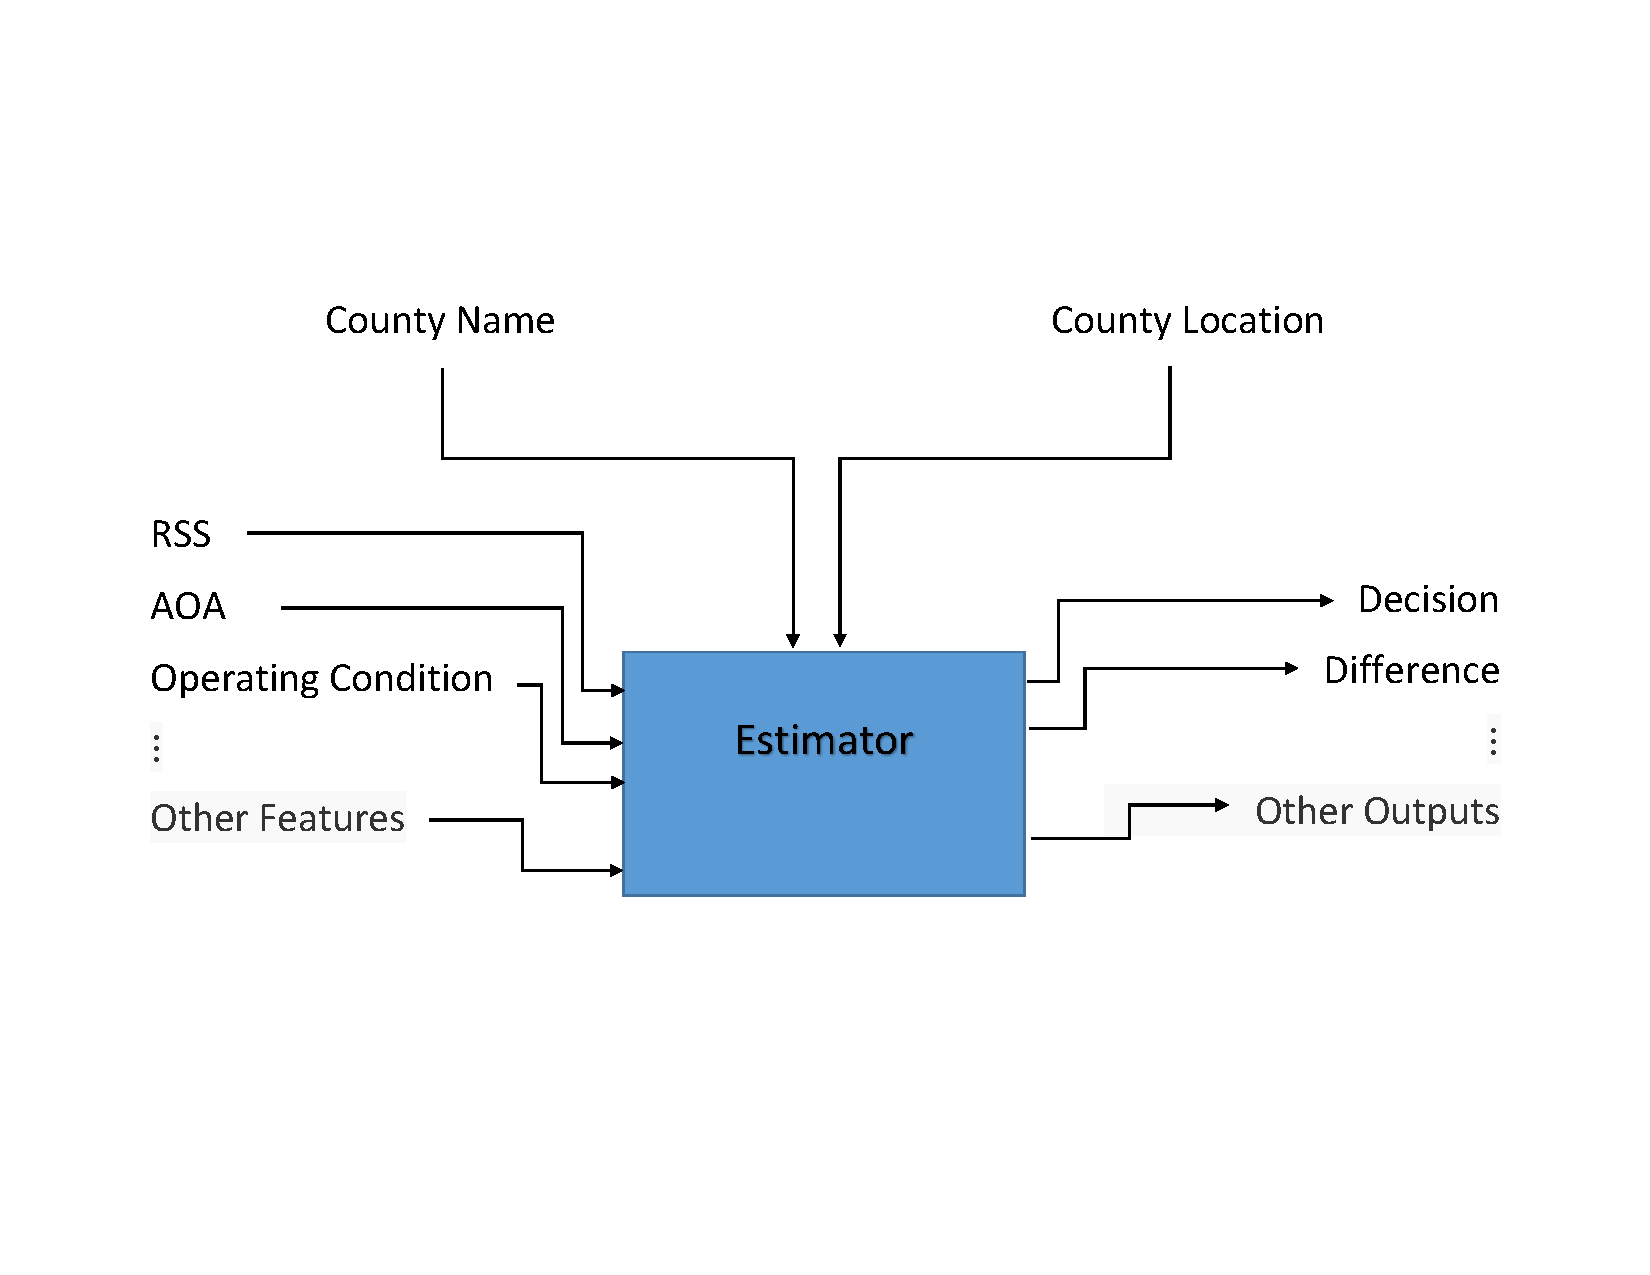
\includegraphics[width=6in]{classifier}
\caption{Second proposed classifier.}
\label{class2}
\end{figure}

A summary of the intended inputs and outputs are given in Fig. \ref{class2}. In order to address two distinctly different styles of application, the proposed method delivers two separate outputs that respectively address the two following questions:

\begin{itemize}
  \item Given a set of different measurement types and the location of a given county, do the measurements belong to said county?
  \item Given a set of different measurement types and the locations of all available counties, which county most closely matches the measurements?
\end{itemize}

\subsection{Accuracy Calculation}

Three different types of accuracy are established in calculating the effectiveness of the two questions posed in the previous subsection: full accuracy, short accuracy, and matching accuracy. Full accuracy refers to the method presented in Subsection 3.4.6 and is based on the first question in the previous subsection. A second accuracy technique, known as short accuracy, is also based on the first question and follows a similar process except that only the matching counties and measurement sets are tested, e.g. county 1 with measurement set 1, county 2 with measurement set 2, etc. The results are recorded in an output vector of length equal to the number of counties, rather than a two-dimensional square matrix of the same side length, and compared against a vector of equal length with values consisting entirely of ones. The two vectors are compared by the same means as before with the same formula as that in Equation \ref{acc}. 

The third accuracy type is based on the second question of the previous subsection, in which a single list of measurements and a full list of all counties are the two inputs and the number corresponding to the most likely county match is the output. To test matching accuracy, every measurement set (in order of their matching county numbers) is tested against the list of counties to form a resultant output vector of size similar to that in short accuracy. The contents of said array take the form of county numbers. This vector is then compared against the ideal vector, which is simply every county number in numerical order, on the basis that the measurement sets are given in the same order. The two matrices are then compared similarly to before with Equation \ref{acc} for calculating accuracy.

\begin{algorithm}
\caption{Pseudocode of DS testing algorithm} \label{alg-test}
\begin{algorithmic}[1]
\STATE test\_data $\leftarrow$ read measured feature values, county name and location, and monitor locations
\STATE full\_data $\leftarrow$ read potential feature values for the county and monitors
\STATE range $\leftarrow$ feature-specific range values for each active feature
\FORALL{measurement sets}
	\FORALL{counties}
		\STATE [decision, difference] $\leftarrow$ outputs of Algorithm 3 using test\_data, full\_data, and range as inputs
	\ENDFOR
	\STATE index $\leftarrow$ minimum difference
	\STATE matching\_county $\leftarrow$ county at index
\ENDFOR
	

\label{dst}
\end{algorithmic}
\end{algorithm}

In order to thoroughly evaluate all three types of accuracy, a simple testing algorithm is formed as portrayed in the pseudocode of Algorithm 5. This technique consists of two $for$ loops, which evaluate the core localization algorithm for all possible combinations of feature sets and counties. The algorithm then extracts all desired differences between measured and calculated distances as well as all matching county outputs required for the three main forms of accuracy calculation.

\section{Results and Discussion}

This section provides the results for the experimental setup and parameters detailed in the previous section, including the preliminary training-based approach intended only for initial WSN implementations as well as the core training-independent approach. The latter of the two serves as the primary focus of discussion due to its elegant combination of flexibly high accuracy and low computational cost.

\subsection{Results Under Distance Range Weight Training}

\begin{figure*}\centering
\subfloat[Full Accuracy\label{fullacc}]
        {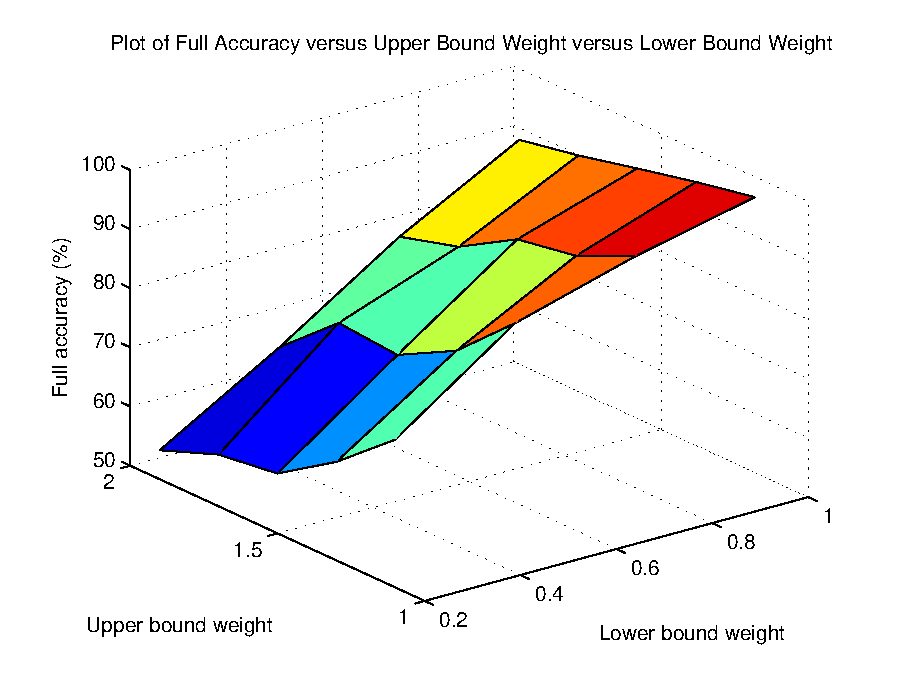
\includegraphics[width=0.45\textwidth]{longacc.eps}}
    \hfill
\subfloat[Short Accuracy \label{shortacc}]
         {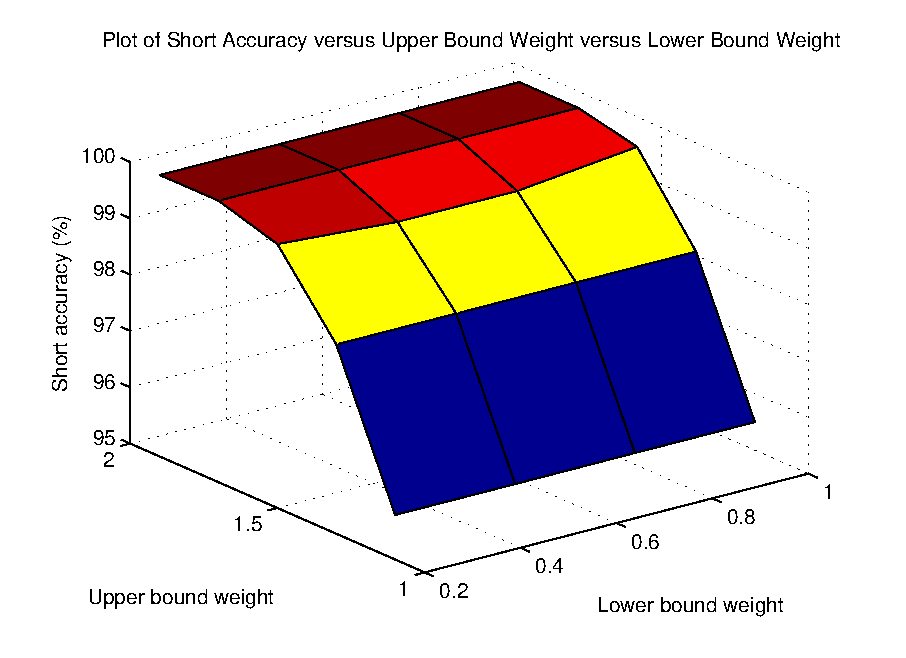
\includegraphics[width=0.45\textwidth]{shortacc.eps}}

\subfloat[Matching Accuracy \label{matchacc}]
         {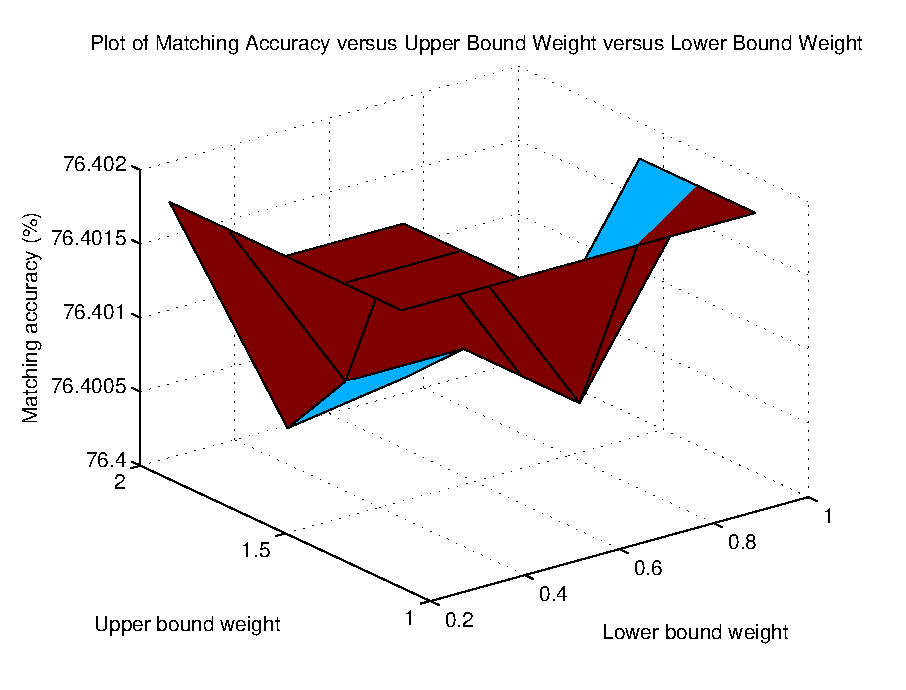
\includegraphics[width=0.45\textwidth]{matchacc.eps}}
    \hfill
\subfloat[Average Accuracy \label{avgacc}]
        {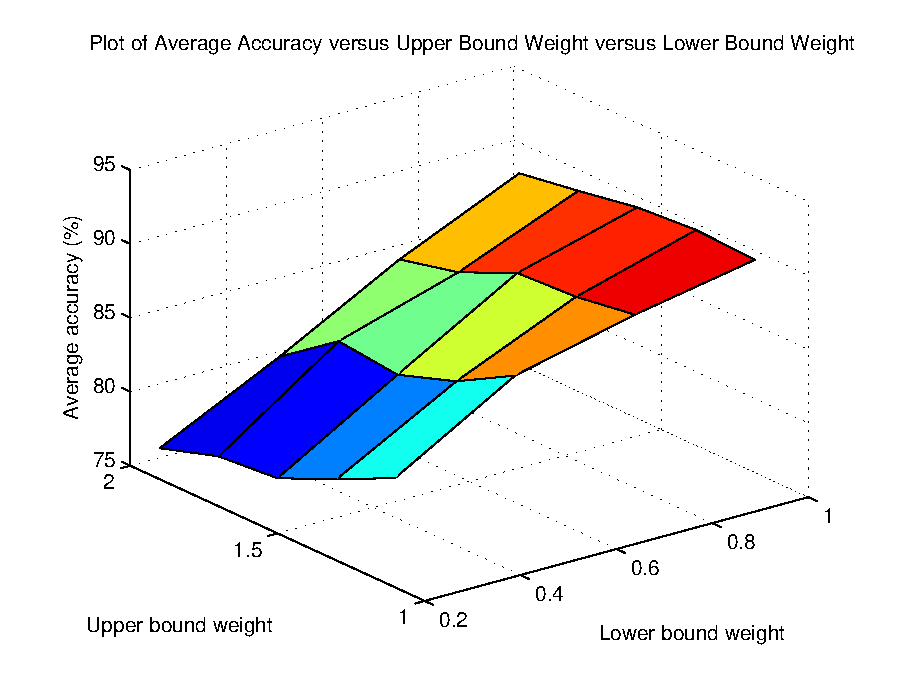
\includegraphics[width=0.45\textwidth]{avg.eps}}
\caption{Plots of accuracy versus upper bound weight versus lower bound weight.}
    \label{train-acc}
    \end{figure*}

The training-based portion of the simulation was trained with 20 possible combinations of desired values, as detailed in Section 3.4. The results for all three accuracy types as well as the averages thereof are presented in Fig.~\ref{train-acc}. Each result is the average of 30 independent trials, that is, three times the amount of trials run in the proceeding subsection. As the surface plots indicate, full accuracy reaches optimal levels when the lower bound weight is maximized and the upper bound weight is minimized. Short accuracy appears to be almost independent of lower bound weight values and optimizes at the maximum upper bound. Matching accuracy follows the most uniform distribution of accuracy values, varying from 76.000\% to 76.002\%, optimizing at multiple possible points, effectively making this form of accuracy negligible in the attempt to find a single best weight combination. The average accuracy is the primary decision factor of weight selection and optimizes upon a maximum lower bound of 0.95 and an upper bound of 1.3, located in a tightly contained region in which average accuracy narrowly exceeds 90\%. Hence, these particular lower and upper weights have been verified to produce the most accurate data and are thus used consistently under the implementation detailed in the following subsection.

\subsection{Training-Independent Results}

The training-independent portion of the simulation was tested in 24 different scenarios resultant from four independent variables: the set of active features, the number of monitors, the type of accuracy, and the trial-based generation of the WSN. The number of monitors used in the simulation were restricted to two and three, as these have been established minimums under unimodal RSS and AOA based localization methods. For reliability and redundancy purposes, the WSN involved in the simulator was re-generated prior to each of the ten experimental trials for each of the above combinations of scenarios. The accuracy results for all test cases are given in Table \ref{table_example}, and the runtime results are provided in Table \ref{table_run_time}, where each value for each table is the average run time for all trials.

\subsubsection{Accuracy}

\begin{table}[!t]
\renewcommand{\arraystretch}{1.3}
\caption{Simulation results for two-monitor and three-monitor WSNs.}
\label{table_example}
\centering
\resizebox{\textwidth}{!}
{\begin{tabular}{*{7}{l}|*{2}{l}}
\toprule
Accuracy  & \multicolumn{2}{l}{Full (\%)} & \multicolumn{2}{l}{Short (\%)} & \multicolumn{2}{l|}{Match (\%)} & \multicolumn{2}{l}{Average (\%)} \\
Monitors & 2 & 3 & 2 & 3 & 2 & 3 & 2 & 3 \\ \midrule
RSS & 97.04 & 97.49 & 97.20 & 98.50 & 56.17 & 66.64 & 83.47 & 87.54 \\
RSS, SB & 97.00 & 97.43 & 100.0 & 100.0 & 94.58 & 96.07 & 97.19 & 97.83 \\
RSS, AOA & 97.03 & 97.47 & 98.13 & 98.97 & 57.81 & 67.29 & 84.33 & 87.92 \\
RSS, AOA, SB & 97.01 & 97.44 & 100.0 & 100.0 & 92.52 & 94.21 & 96.51 & 97.22 \\ \bottomrule
\end{tabular}}
\end{table}

As Table \ref{table_example} indicates, the full accuracy test generates consistently high results in the steady area of 97.0-97.5\% accuracy for all eight scenarios, thereby proving the algorithm to be consistently effective for both two-monitor and three-monitor setups under all feasible combinations of active features. Results of the short accuracy test climb even higher with a value range of 97-100\%. Under the matching accuracy test, results span a wider range of accuracy results from 56.1\% to 94.6\%. The average of all three accuracy types indicate a somewhat less diverse range of 83.5\% to 97.8\%. The results ultimately indicate that the matching of counties works most effectively when only RSS and operating condition are enabled, as the absence of operating condition results in the only accuracy values lower than 94\% as well as the only short accuracy values that are below 100\%. 

The full accuracy test is one evaluation that does not appear to fully benefit from data fusion. While fusing multiple types of data is intended to enhance an accuracy relative to that of a single type of data, this test shows that full accuracy is most effective when only RSS data is available. The other evaluation methods, however, clearly show that fusion of multiple measurement types do in fact enhance accuracy. Combining this observation with the fact that differences in full accuracies are minimal (all values for each monitor are within 0.06\% of one another) can easily infer that data fusion in this context is still an overall success. 

Also worth noting is that RSS as a sole feature forms the weakest accuracy and may pale in comparison to traditional RSS-based localization when only RSS is available. One should keep in mind, however, that all other remaining feature combinations, that is, any combination of two or more features, proves that fusion of multiple available types of data in this algorithm is significantly more effective than any conventional unimodal technique. Because the scope of this research focuses primarily on the advantages of fusing multiple different types of data, the results for RSS as the sole available feature should therefore be considered of least importance.

Another successful outcome is the high accuracy involved in two-monitor WSNs. Most established localization methods require three or more monitors to observe a sensor node's measurements, but in this algorithm, two-monitor WSNs can localize reliably with a less-than-0.5\% decrease in accuracy. From the standpoint of having RSS as the only enabled feature, achieving a high accuracy with three monitors is trivial, as this can be achieved purely through trilateration. Under two monitors, however, only bilateration is available, meaning that if distance values calculated from RSS measurements are exact, there is still only a 50\% chance of obtaining the correct location. Thus, with DS Theory, highly accurate localization can be achieved just as easily with only two monitors as it can with three or more.

\subsubsection{Computational Runtime}

\begin{table}[!t]
\renewcommand{\arraystretch}{1.3}
\caption{Runtime results for two-monitor and three-monitor WSNs.}
\label{table_run_time}
\centering
$\begin{tabular}{*{3}{l}}
\toprule
Runtime (ms) & 2 Monitors & 3 Monitors\\ \midrule
Total & 787478.00 & 1375261.00 \\
Per Feature Set & 196869.00 & 343815.20 \\
Per Iteration & 17.20 & 30.03 \\
Per Node & 0.160 & 0.281 \\ 
\bottomrule
\end{tabular}$
\end{table}

Total runtime for an entire simulation for all four available feature sets combined was recorded for each trial. From there, the calculated time was averaged per feature set, then divided by all $100^2=10000$ possible input combinations to find the average runtime per iteration. Finally, the latter runtime was divided by all 100 nodes to find the average runtime per node. All four types of runtimes were averaged for all ten trials and then recorded in Table \ref{table_run_time} for both two-monitor and three-monitor WSNs. Each trial was run on consistent computer hardware and software, including a standard Windows version of MATLAB on a quad core 2.60 GHz processor and 8.0 GB of RAM. The significance of these results will be explained in greater detail upon the next subsection.

\subsection{Comparisons to Other Established Algorithms}

\begin{table}
\renewcommand{\arraystretch}{1.3}
\caption{Comparison of accuracy among different localization techniques.}
\label{compare2}
\centering
$\begin{tabular}{*{7}{l}}
\toprule
Algorithm & PSO & WSLA & WSRA & MLE & DS1 & DS2 \\
\midrule
Accuracy (\%) & 71 & 90 & 92 & 93 & 87 & 97 \\
Runtime ($\mu$s) & 114570 & 7800 & 9700 & NR & 12733 & 281 \\
\bottomrule
\end{tabular}$
\end{table}

To gain further perspective into this technique's effectiveness, comparisons were made to the four prior established localization methods presented in the previous chapter as well as the proposed DS-based technique of said chapter. In Table \ref{compare2}, the previous method is still referred as DS1 while the currently presented technique is labelled as DS2.

\subsubsection{Accuracy}

As the first row of data in Table \ref{compare2} indicates, the proposed technique contains a noticeable edge in accuracy in comparison to the other methods as well as a significant lead over PSO and DS1. Although some parameters had to be tweaked between this method and the others, a fair conclusion can be made that this DS-based algorithm has a distinct advantage on par with, if not over, multiple established state-of-the-art localization techniques.

\subsubsection{Computational Runtime}

Average run time per node for a three-monitor WSN setup was compared with three of the four aforementioned techniques, based on data given in \cite{yao}. All method runtimes, sans that of MLE, are reported in the second row of data in Table \ref{compare2}. As the table plainly indicates, the proposed method has an overwhelmingly shorter CPU runtime than all reported competing methods, hence solidifying such an algorithm as a novel low cost technique.

\section{Conclusions}

In this chapter, a novel approach to localization in wireless sensor networks was presented. This approach was based heavily upon the innovative statistical framework known as Dempster-Shafer Evidence Theory. While DS Theory contains many unique properties that can aid in data prediction and analysis, the concept of prediction by plausibility is of the most vital levels of importance and interest, due to its consistently high accuracy under a variety of network setups and feature set availabilities as well as its considerably low computational cost requirements.

% CHAPTER FIVE

\chapter{Conclusive Remarks}

The end goal of this research was to investigate the concepts and applications of Dempster-Shafer Theory and incorporate such a method into the development of novel, computationally attractive algorithms for wireless sensor network localization. Hence, two new localization schemes were presented in Chapters 3 and 4. 

The first technique, proposed in Chapter 3, served as a verbose, introductory method of moderate accuracy with the primary objective of merely wading in the untapped waters that form Dempster-Shafer-based WSN localization. This method of node positioning functioned by fusing multiple types of signal measurements, such as received signal strength and angle of arrival, and executing the expected value function of DS Theory to predict a range of distances for multiple monitors, through which a feasible region could be obtained, thereby detailing a list of coordinates among which the targeted node could lie. The algorithm produced an accuracy of 78-87\% across a multitude of feature selection scenarios, thereby providing an adequate introductory approach to the previously untapped fusion of WSN localization and DS Theory. This new approach is primarily intended to aid in future research and development of Dempster-Shafer-based localization techniques, such as the one proposed in Chapter 4. In addition, however, this technique can also be utilized in practicality for applications in which obtaining a desired region of potential geo-location is more strongly desired than estimating a specific point.

In Chapter 4, a second method was presented with a significantly higher accuracy and exponentially lower computational cost. This method used the plausibility function of DS theory, rather than expected value, to generate a most plausible distance from node to monitor and use an optimal range of values proportional to the most plausible value in order to determine whether a set of measurements belong to a given county. This technique produced 83-98\% accuracy for a multitude of feature selection criteria as well as multiple anchor node setups. 

Time-critical localization of WSNs is a topic of increasing concern in today's world, as a variety of civil and military applications can thrive on low-cost, high-accuracy localization techniques. Recall from Chapter 1 the example of a city-wide network of emergency phones, connected wirelessly for the sake of low overhead with regards of hardware. Using effective localization techniques such as that proposed in Chapter 4, 911 services can dispatch police, fire, or medical services to a caller's exact location as quickly as humanly possible. Hence, the uniqueness and effectiveness of this novel algorithm can have a crucial impact on today's world, as every percent of accuracy achieved and every second of time saved can be the difference between life and death.

\section{Future Work}

Due to the groundbreaking, cutting edge research potential of Dempster-Shafer Theory, as demonstrated by the previous chapter of this thesis, the resultant research thereof has the potential to diverge into many possible future directions.

\subsection{Enhanced Training of Upper and Lower Bound Coefficients}

Training of the upper and lower bound weights was done from a limited iterative approach. Although this brief technique resulted in multiple high levels of accuracy above 90\%, accuracy could be even further enhanced through more elaborate optimization methods, similar to those utilized in neural network training. Possibilities include local methods, such as Steepest Descent or Conjugate Gradient, as well as global, biologically inspired methods, such as Genetic Algorithm or Ant Colony Optimization.

\subsection{Fusion of DS Theory With Support Vector Machines}

Support vector machines (SVMs) have been of a high level of interest in the field of WSN localization, almost to the same extent as DS Theory, due to its fast localization potential and efficient use of processing resources. Because the end goal of the National Science Foundation grant supporting this research involves the fusion of DS Theory with SVMs, the most logical next step of this research will be to develop WSN localization schemes based upon such a combination of techniques.

\subsection{Role of DS Theory Within Data Mining and Big Data Analytics}

Data mining, or big data, is another method of predictive data analysis, as previously addressed in Section 3.1 and is of overwhelmingly significant interest in the modern technological world, primarily due to the growing need for the handling and processing of immense quantities of data. In many applications, however, the necessity arises to supplement data mining paradigms with additional predictive data models by the process of meta-learning. Many typical methods that are included in meta-learning include tree classifiers, linear analysis, and neural networks. Because Dempster-Shafer Theory is a predictive model that is still inching its way into new and innovative applications (as is clearly the case with WSN localization), the inclusion of DS Theory as a meta-learning mechanism could be highly beneficial to the effectiveness of many big data methods.



%XXXXXXXXXXXXXXXXXXXXXXXXXXXXXXXXXXXXXXXXXXXXXXXXXXXXXXXXXXXXXXXXXXXX
%XXXXXXXXXXXXXXXXXXXXXXXXXXXXXXXXXXXXXXXXXXXXXXXXXXXXXXXXXXXXXXXXXXXX
%XXXXXXXXXXXXXXXXXXXXXXXXXXXXXXXXXXXXXXXXXXXXXXXXXXXXXXXXXXXXXXXXXXXX
%XXXXXXXXXXXXXXXXXXXXXXXXXXXXXXXXXXXXXXXXXXXXXXXXXXXXXXXXXXXXXXXXXXXX

%--------+----------------------------------------------------------+
%        |  \myreferences{}                          (CONDITIONAL)  |
%        |                                                          |
%        |  See section 3.18 of "Read_Me_First_(v12).pdf"           |
%        |                                                          |
%        |  That section of the READ ME file describes two options  |
%        |  for listing the works cited in your document: first,    |
%        |  manually entering your list of references and, second,  |
%        |  using BibTeX to generate that list.                     |
%        |                                                          |
%        |  1) If you manually enter your reference list, first     |
%        |     include the \myreferences command, as illustrated    |
%        |     below.  Second, use the "referencelist" environment  |
%        |     described below.  For this, note that the UT Manual  |
%        |     requires double-spacing *between* references in      |
%        |     that list. However, it also states that *within*     |
%        |     individual references the spacing may be single- or  |
%        |     double-spaced.  Because of this, UThesis provides    |
%        |     two options for the "referencelist" environment:     |
%        |                                                          |
%        |            \begin{referencelist}{ENTER OPTION HERE}      |
%        |            \item ...                                     |
%        |            \end{referencelist}                           |
%        |                                                          |
%        |     a. Replacing "ENTER OPTION HERE" above with the      |
%        |        text "single" will generate a reference list      |
%        |        with single-spaced entries in that list but       |
%        |        double-spacing between those entries. An example  |
%        |        of this is provided below.                        |
%        |     b. Alternatively, using the "double" option will     |
%        |        generate a list with double-spaced entries and    |
%        |        double-spacing between entries. An example of     |
%        |        this is also provided below.                      |
%        |                                                          |
%        |     Note that input to these options is case sensitive   |
%        |     and the default setting is the "double" option.      |
%        |                                                          |
%        |  2) If you instead choose to use BibTeX to generate the  |
%        |     reference list, then you *cannot* include either     |
%        |     the "\myreferences" command or the "referencelist"   |
%        |     environment in your document. In this case you must  |
%        |                                                          |
%        |     a. delete the \myreferences command and the two      |
%        |        examples of the "referencelist"  environment      |
%        |        below;                                            |
%        |     b. then you must add and locate appropriately all    |
%        |        necessary BibTeX commands within your document    |
%        |        (e.g., \bibliographystyle{}, \citationstyle{},    |
%        |        \bibliography{}, etc.).                           |
%        +----------------------------------------------------------+



\begin{thebibliography}{00}

%% \bibitem{label}
%% Text of bibliographic item

\bibitem{pivato}
Pivato, P., Palopoli, L., and D. Petri (2011) ``Accuracy of RSS-Based Centroid  Localization Algorithms in an Indoor Environment,'' {\it IEEE Transactions on Instrumentation and Measurement, 60(10)}, 3451--3460.

\bibitem{dhan}Dhanaraj, M. and Murthy, C. (2007) ``On Achieving Maximum Network Lifetime Through Optimal Placement of Cluster-heads in Wireless Sensor Networks'', {\it IEEE International Conference on Communications}, 3142-3147. 

%\bibitem{zhang1}
%Zhang, Y., Meratnia, N., and Havinga, P. (2009) Adaptive and Online One-Class Support Vector Machine-Based Outlier Detection Techniques for Wireless Sensor Networks. {\it International Conference on Advanced Informational Networking and Applications Workshops}, 990-995.

%\bibitem{zhang4}
%Zhang C., Cui P., and Zhang, Y. (2006) An Algorithm of Data Fusion Combined Neural Networks with DS Evidential Theory. {\it 1st International Symposium on Systems and Control in Aerospace and Astronautics}, 1141-1144.

\bibitem{patel}
Patel, T., Udayakumar, P., and Ranjana, V. (2015) ``Analyzing Data Mining Techniques for Wireless Sensor Network Protocols,'' {\it International Conference on Computing for Sustainable Global Development, 2}, 1673-1678.

\bibitem{peng}
Peng, R. and Sichitiu, M. (2006) ``Angle of Arrival Localization for Wireless Sensor  Networks,'' {\it IEEE Communications Society on Sensor and Ad Hoc  Communications and Networks, 1}, 374--382.

\bibitem{yang2}
Yang, L. and Ho, K. (2009) ``An Approximately Efficient {TDOA} Localization  Algorithm in Closed-Form for Locating Multiple Disjoint Sources with Erroneous Sensor Positions,'' {\it IEEE Transactions on Signal Processing, 57(12)}, December 2009, 4598--4615. 

\bibitem{song}
Song, H. (1994) ``Automatic Vehicle Location in Cellular Communication System'', {\it IEEE Transactions on Vehicular Technology, 43(4)}, 902-908.

\bibitem{chiodo1}
Chiodo, E., Lauria, D., Pisani, C. (2014) Bayes Estimation of Wind Speed Extreme Values. {\it 3rd Renewable Power Generation Conference (RPG 2014)}, 1-7.

\bibitem{luo} Luo, Y. and Xiaoyi, C. (2009) ``Chaos Immune Particle Swarm Optimization Algorithm with Hybrid Discrete Variables and its Application to Mechanical Optimization'', {\it International Symposium on Intelligent Information Technology Application Workshops}, 190-193.

\bibitem{liu}
Liu, C., Huo, H., Fang, T., Li, D., and Shen, X. (2006) ``Classification Fusion in Wireless Sensor Networks,'' {\it ACTA Automatica Sinica, 32(6)}, 947-955.

\bibitem{sarinnapakom}
Sarinnapakom, K. and Kubat, M. (2007) ``Combining Subclassifiers in Text Categorization: A DST-Based Solution and a Case Study,'' {\it IEEE Transactions on Knowledge and Data Engineering, 19(12)}, 1638-1651.

%\bibitem{zhang2}
%Zhang, F., Guilherme, P., and Kumar, V. (2005) Cooperative Localization and Tracking in Distributed Robot-Sensor Networks. {\it Tsinghua Science and Technology, 10(1)}, 91-101.

\bibitem{nguyen}
Nguyen, H. and Walker, E. (1993) ``On Decision-Making using Belief Functions,'' {\it In Advances in the Dempster-Shafer Theory of Evidence}, 311-330.

\bibitem{beynon}
Beynon, M., Curry, B., and Morgan, P. (2000) ``The Dempster-Shafer Theory of Evidence: An Alternative Approach to Multicriteria Decision Modelling,'' {\it Omega: The International Journal of International Science, 28(1)}, 37-50.

%\bibitem{murphy}
%Murphy, R. (1998) Dempster-Shafer Theory for Sensor Fusion in Autonomous Mobile Robots. {\it IEEE Transactions on Robotics and Automation, 14(1)}, 197-205.

\bibitem{xu}
Xu, J., Liu, W., Lang, F., Zhang, Y., and Wang, C. (2010) ``Distance Measurement Model Based on RSSI in WSN,'' {\it Wireless Sensor Network, 2(8)}, 606-611.

\bibitem{zhang5}
Zhang, W., Yin, Q., Chen, H., Gao, F., and Ansari, N. (2013) ``Distributed Angle Estimation for Localization in Wireless Sensor Networks,'' {\it IEEE Transtions on Wireless Communications, 12(2)}, 527--537.

%\bibitem{dima}
%Dima, S., Panagiotou, C., Tsitsipis, D., Antonopoulos, C., Gialelis, J., and Koubias, S. (2014) Performance Evaluation of a WSN System for Distributed Event Detection Using Fuzzy Logic. {\it Ad Hoc Networks, 23}, 87-108.

\bibitem{yao}
Yao, Y., Jiang, N. (2015) ``Distributed Wireless Sensor Network Localization Based on Weighted Search,'' {\it Computer Networks}, 1-26.

\bibitem{chiodo2}
Chiodo, E. and Lauria, D. (2014) ``Double Stochastic Analysis of Batteries Lifetime for Electric Vehicles Operation,'' {\it 3rd Renewable Power Generation Conference (RPG 2014)}, 1-7.

%\bibitem{li}
%Li, S., Qin, F. (2013) A Dynamic Neural Network Approach for Solving Nonlinear Inequalities Defined on a Graph and Its Application to Distributed, Routing-Free, Range-Free Localization of WSNs. {\it Neurocomputing, 117}, 72-80.

\bibitem{rish}
L. Rish (2001) ``An Empirical Study of the Naive Bayes Classifier'', {\it Workshop on Empirical Methods in Artificial Intelligence}, 2001, 41-46.

\bibitem{desh}Deshpande, V. and Patil, A. (2013) ``Energy Efficient Clustering in Wireless Sensor Network using Cluster of Cluster Heads'', {\it 2013 Tenth International Conference on Wireless and Optical Communications Networks (WOCN)}, 1-5.

%\bibitem{aslandogan}
%Aslandogan, Y. (2004) Evidence combination in medical data mining. {\it International Conference on Information Technology: Coding and Computing, 2}, 465-469.

\bibitem{hwang}
Hwang, D., Hwang, J., Jang, S., and Kim, J. (2009) ``A Fast ToA Position Estimation Technique Based on MHP Pulse,'' {\it 9th International Symposium on Communications and Information Technology}, 1472-1476.

%\bibitem{zhi}
%Zhi, W. (2011) Fault Diagnosis for Wireless Sensor Network Based On Genetic-Support Vector Machine. {\it International Conference on Computer Science and Network Technology, 4}, 2691-2694.

\bibitem{limbourg}
Limbourg, P., Savic, R., Petersen, J., and Kochs, H. (2007) ``Fault Tree Analysis In An Early Design Stage Using the Dempster-Shafer Theory of Evidence,'' {\it Risk, Reliability and Societal Safety}, 713-722.

\bibitem{yang2}
Yang, G., Yi, Z., Tmnquan, N., Keke, Y., and Tongtong, X. (2010) ``An Improved Genetic Algorithm for Wireless Sensor Networks Localization,'' {\it IEEE Fifth International Conference on Bio-Inspired Computing}, 439-443.

\bibitem{yi}
Yi, C., Qing, H., Yanlan, C. (2012) ``An Improve Information Fusion Algorithm Based on BP Neural Network and D-S Evidence Theory,'' {\it Third International Conference on Digital Manufacturing \& Automation}, 179-181.

%\bibitem{lipeng}
%Lipeng, G., Juan, J., and Laibin, D. (2011) An Improved Algorithm of Evidence Theory. {\it Cross Strait Quad-Regional Radio Science and Wireless Technology Conference, 2}, 1495-1498.

\bibitem{deng}
Deng, Y., Wang, D., and Li, Q. (2008) ``An Improved Combination Rule in Fault Diagnosis Based on Dempster-Shafer Theory,'' {\it Proceedings of the Seventh International Conference on Machine Learning and Cybernetics, 1}, 212-216.

\bibitem{kumarasiri1}
Kumarasiri, R., Alshamaileh, K., Tran, N., and Devabhaktuni, V. (2015) ``An improved Hybrid RSS/TDOA Wireless Sensor Localization Technique Utilizing Wi-Fi Networks,'' {\it Mobile Networks and Applications}.

%\bibitem{xueji}
%Xueji, T. and Li, Y. (2010) An Improved Fusion Algorithm Of Evidence Theory. {\it 2nd Conference on Environmental Science and Information Application Technology}, 400-402.

%\bibitem{bi}
%Bi. Y, McClean, S., and Anderson, T. (2005) Improving classification decisions by multiple knowledge. {\it 17th IEEE Conference on Tools with Artificial Intelligence}, 340-347.

\bibitem{nakamura}
Nakamura, E., Loureiro, A., and Frery, A. (2007) ``Information Fusion for Wireless Sensor Networks: Methods, Models, and Classifications,'' {\it ACM Computing Surveys, 39(3)}, 1-55.

\bibitem{agrawal}
Agrawa, D. P. and Zeng, Q. (2011) {\it Introduction to Wireless and Mobile Systems} (4th ed.). Stamford: Cengage Learning, (Chapter 14).

\bibitem{cakir}
Cakir, O., Kaya, I., and Cakir, O. (2014) ``Investigation the Effect of the Time Difference of Arrival Sets on the Positioning Accuracy for Source Localization,'' {\it Signal Processing and Communications Applications Conference (SIU)}, 2249-2252.

\bibitem{ipp}
{\it Imprecise Probability Propagation Toolbox (IPP Toolbox)} (2012) Essen, Germany: University of Duisberg-Essen, Department of Information Logistics, (https://www.uni-due.de/informationslogistik/ipptoolbox.php). Last accessed June 1, 2015.

\bibitem{dapeng}Dapeng, Q. and Pang, G. (2011) ``An iteratively Reweighted Least Square algorithm for RSS-based sensor network localization,'' {\it 2011 International Conference on Mechatronics and Automation (ICMA)}, 1085-1092.

%\bibitem{eriksson}
%B. Eriksson, P. Barford, J. Sommers, and R. Nowak (2010) `A learning-based approach for IP geolocation,' {\it Passive and Active Measurement Workshop}, 2010.

\bibitem{so}
So, H. and Lin, L. (2011) ``Linear Least Squares Approach for Accurate Received Signal Strength Based Source Localization,'' {\it IEEE Transactions on  Signal Processing, 59(8)}, 4035--4040.

\bibitem{patwari}
Patwari, N., Ash, J., Kyperountas, S., Hero, A., Moses, R., and Correal, N. (2005) ``Locating the Nodes: Cooperative Localization in Wireless Sensor Networks,'' {\it IEEE Signal Processing Magazine, 22(4)}, 54-69.

\bibitem{kumarasiri2}
Kumarasiri, R., Elkin, C., Shamaileh, K. Shetty, S., Tran, N., and Devabhaktuni, V. (Unpublished results) ``Low Cost Data Fusion Technique for Localization in Wireless Sensor Network,'' {\it Transactions on Emerging Telecommunications Technologies}.

%\bibitem{tran}
% A. D. Tran and T. Nguyen (2008) `Localization In Wireless Sensor Networks Based on Support Vector Machines,' {\it IEEE Transactions on Parallel and Distributed Systems}, Vol. 19 , No. 7, July 2008, pp. 981--984.

\bibitem{gopa}
Gopakumar, A, and Lillykutty, J. (2008) ``Localization in Wireless Sensor Networks Using Particle Swarm Optimization,'' {\it International Conference on Wireless, Mobile and Multimedia Networks}, 227--230. 

\bibitem{ding}
Ding, H., Chen, H., Zhuang, H., and He, X., (2014) ``Localization in WSN using maximum likelihood estimation with negative constraints based on particle swarm optimization,'' {\it 2014 12th International Conference on Signal Processing (ICSP)}, 19-23.

%\bibitem{zhang3}
%Zhang, B. and Yu, F. (2010) LSWD: Localization Scheme for Wireless Sensor Networks using Directional Antenna. {\it IEEE Transactions on Consumer Electronics, 56(4)}, 2208-2216.

\bibitem{matlab}
{\it MATLAB version 8.1} (2013) Natick, Massachusetts: The MathWorks Inc.

\bibitem{kim} Kim, J., Lee, J., and Park, C. (2008) ``A Mitigation of Line-of-Sight by TDOA Error Modeling in Wireless Communication System.'', {\it International Conference on Control, Automation and Systems}, 1601-1605.

%\bibitem{sun}
%Sunantasaengtong, P., Chivapreecha, S. (2014) Mixed K-means and GA-based weighted distance fingerprint algorithm for indoor localization system. {\it TENCON 2014 - 2014 IEEE Region 10 Conference}, 22-25.

%\bibitem{rodriguez}
%Rodriguez, S., De Paz, J., Villarrubia, G., Zato, C., Bajo, J., Corchado, J. (2015) Multi-Agent Information Fusion System to Manage Data from a WSN in a Residential Home. {\it Information Fusion, 23}, 43-57.

\bibitem{pelant}
Pelant, M., Stejskal, V. (2011) ``Multilateration System Time Synchronization via Over-Determination of TDOA Measurements,'' {\it 2011 Tyrrhenian International Workshop on Digital Communications - Enhanced Surveillance of Aircraft and Vehicles (TIWDC/ESAV)}, 12-14.

%\bibitem{shen2}
%H. Shen, Z. Ding, S. Dasgupta, and C. Zhao (2014) `Multiple Source Localization in Wireless Sensor Networks Based on Time of Arrival Measurement,' {\it IEEE Transactions on Signal Processing}, Vol. 62 , No. 8, April 2014, pp. 1938--1949.

\bibitem{wang}
Wang, Y., Chu, F., He, Y., and Guo, D. (2004) ``Multisensor Data Fusion for Automotive Engine Fault Diagnosis,'' {\it Tsinghua Science and Technology, 9(3)}, 262-265.

\bibitem{al-ani}
Al-Ani, A., and Deriche, M. (2002) ``A New Technique for Combining Multiple Classifiers using The Dempster-Shafer Theory of Evidence,'' {\it Journal of Artificial Intelligence Research, 17}, 333-361.

%\bibitem{safa}
%Safa, H. (2014) A Novel Localization Algorithm for Large Scale Wireless Sensor Networks. {\it Computer Communications, 45}, 32-46.

\bibitem{ibrahim}
Ibrahim, I., Yusof, Z., Nawawi, S., Rahim, M., Ahmad, H., and Ibrahim, Z. (2012) ``A Novel Multi-state Particle Swarm Optimization for Discrete Combinatorial Optimization Problems,'' {\it Fourth International Conference on Computational Intelligence, Modelling and Simulation (CIMSiM)}, 18-23.

%\bibitem{yang}
%Yang, Z., Meratnia, N., and Havinga, P. (2008) An Online Outlier Detection Technique for Wireless Sensor Networks Using Unsupervised Quarter-Sphere Support Vector Machine. {\it International Conference on Intelligent Sensors, Sensor Networks and Information Processing}, 151-156.

%\bibitem{kazemi}
%Kazemi, I., Moniri, M., and Kandovan, S. (2013) Optimization of Angle-of-Arrival Estimation Via Real-Valued Sparse Representation With Circular Array Radar. {\it IEEE Access, 1}, 404-407.

%\bibitem{wang}S. Wang, B. Jackson, and R. Inkol (2012) `Performance Characterization of AOA Geolocation Systems Using the Von Mises Distribution', {\it 2012 IEEE Vehicular Technology Conference (VTC Fall)}, September 2012, pp. 1-5.

\bibitem{hatami}A. Hatami and K. Pahlavan (2006) ``Performance Comparison of RSS and TOA Indoor Geolocation Based on UWB Measurement of Channel Characteristics,'' {\it 17th International Symposium on Personal, Indoor and Mobile Radio Communications}, 1-6.

\bibitem{shafer}
Shafer, G. (1990)``Perspectives on the Theory and Practice of Belief Functions,'' {\it International Journal of Approximate Reasoning, 4(5-6)}, 323-362.

\bibitem{hara} Hara, G.,Anzai, D., Yabu, T., Derham, T., and Zemek, R. (2013) ``A Perturbation Analysis on the Performance of TOA and TDOA Localization in Mixed LOS/NLOS Environments,'' {\it IEEE Transactions on Communications, 61(2)}, 679-689.

%\bibitem{dima}
%Dima S., Panagiotou, C., Tsitsipis, D., Antonopoulos, C., Gialelis, J., and Koubias, S. (2014) Performance Evaluation of a WSN System for Distributed Event Detection using Fuzzy Logic. {\it Ad Hoc Networks, 23}, 87-108.

%\bibitem{wickramaratna}
%Wickramaratna, K., Kubat, M., and Premaratne, K. (2009) Predicting Missing Items in Shopping Carts. {\it IEEE Transactions on Knowledge and Data Engineering, 21(7)}, 985-998.

\bibitem{di}
Di, M., Joo, E., Bang, W., and Beng, L. (2009) ``Range-Free Localization Based on Hop-Count Quantization in Wireless Sensor Networks,'' {\it TENCON 2009 IEEE Region 10 Conference}, 23-26.

\bibitem{yan}T. Yan, Y Tao, and D. Cui (2007) ``Research on Handwritten Numeral Recognition Method Based on Improved Genetic Algorithm and Neural Network,'' {\it International Conference on Wavelet Analysis and Pattern Recognition}, 1271-1276.

\bibitem{mazuelas}
Mazuelas, S., Bahillo, A., Lorenzo, R., Fernandez, P., Lago, F., Garcia, E., Blas, J., and Abril, E. (2009) ``Robust Indoor Positioning Provided by Real-Time RSSI Values in Unmodified WLAN Networks,'' {\it IEEE Journal of Selected Topics in Signal Processing, 3(5)}, 821-831.

\bibitem{cheng} Cheng, W., Kefeng, T., Omwando, V., Zhu, J., and Mohapatra, P. (2013) ``RSS-Ratio for Enhancing Performance of RSS-Based Applications,'' {\it 2013 Proceedings IEEE INFOCOM}, 3075-3083.

%\bibitem{zhou}
%Zhou, Z., Peng, Z., Cui, J., Shi, Z., and Bagtzoglou, A. (2011) Scalable Localization with Mobility Prediction for Underwater Sensor Networks. {\it IEEE Transactions on Mobile Computing, 10(3)}, 335-348.

\bibitem{bhatt}
Bhatt, D., Aggarwal, P., Devabhaktuni, V., and Bhattacharya, P. (2012) ``Seamless Navigation via Dempster Shafer Theory Augmented by Support Vector Machines,'' {\it Proceedings of the 25th International Technical Meeting of The Satellite Division of the Institute of Navigation}, 98-104.

\bibitem{soleimanpour}
Soleimanpour, S., Ghidary, S., and Meshgi, K. (2008) ``Sensor Fusion in Robot Localization using DS-Evidence Theory with Conflict Detection using Mahalanobis Distance,'' {\it 7th IEEE International Conference on Cybernetic Intelligent Systems}, 1-6.

\bibitem{chan}
Chan, Y. and Ho, K. (1994) ``A Simple and Efficient Estimator for Hyperbolic  Location,'' {\it IEEE Transactions on Signal Processing, 42(8)}, 1905--1915.

\bibitem{gkou}
Gkoutioudi, K. and Karatza, H. (2012) ``A Simulation Study of Multi-criteria Scheduling in Grid Based on Genetic Algorithms,'' {\it IEEE 10th International Symposium on Parallel and Distributed Processing with Applications (ISPA)}, 317-324.

%\bibitem{yun}
%Yun, S., Lee, J., Chung, W., Kim, E., and Kim, S. (2009) A Soft Computing Approach {\it Expert Systems with Applications, 36}. 7552-7561.

\bibitem{almaadeed}
Almaadeed, N, Aggoun, A, and Amira, A. (2015) ``Speaker Identification using Multimodal Neural Networks and Wavelet Analysis,'' {\it IET Biometrics, 4(1)}, 18-28.

\bibitem{beyme}
Beyme, S., Jeung, C. (2014) ``A Stochastic Process Model of the Hop Count Distribution in Wireless Sensor Networks,'' {\it Ad Hoc Networks, 17}, 60-70.

%\bibitem{moha} 
%D. Mohapatra and S. Suma (2005) `Survey of location based wireless services', {\it IEEE International Conference on Personal Wireless Communications}, pp. 358--362.

\bibitem{lee} Lee, J., Kim, D., Toh, C., Kwon, T., and Choi, Y. (2005) ``A Table-Driven AOA Estimation Algorithm for Switched-beam Antennas in Wireless Networks', {\it 11th European Wireless Conference 2005 - Next Generation Wireless and Mobile Communications and Services (European Wireless)},'' 1-6.

\bibitem{feng}
Feng, R., Xu, X., Zhou, X., and Wan, J. (2011) ``A Trust Evaluation Algorithm for Wireless Sensor Networks Based on Node Behaviors and D-S Evidence Theory,'' {\it Sensors, 11(2)}, 1345-1360.

%\bibitem{kapplan}E. Kapplan (1996) `Understanding GPS, principal and applications', {\it Artech House}.

\bibitem{dempster}
Dempster, A. (1967) ``Upper and Lower Probabilities Induced by a Multivalued Mapping,'' {\it The Annals of Mathematical Statistics, 2}, 325-339.

\bibitem{tonon}
Tonon, F. (2004). ``Using Random Set Theory to Propagate Epistemic Uncertainty Through a Mechanical System,'' {\it Reliability Engineering and System Safety,  85(1-3)}, 169-181.

\bibitem{auer}
Auer, E., Luther, W., Rebner, G., and Limbourg, P. (2010) ``A Verified MATLAB Toolbox for the Dempster-Shafer Theory,'' {\it Workshop on the Theory of Belief Functions}.

\bibitem{shen}
Shen, X., Chen, W., and Lu, M. (2008) ``Wireless Sensor Networks for Resources Tracking at Building Construction Sites,'' {\it Tsinghua Science and Technology, 13(1)}, 78-83.

\end{thebibliography}

%XXXXXXXXXXXXXXXXXXXXXXXXXXXXXXXXXXXXXXXXXXXXXXXXXXXXXXXXXXXXXXXXXXXX
%XXXXXXXXXXXXXXXXXXXXXXXXXXXXXXXXXXXXXXXXXXXXXXXXXXXXXXXXXXXXXXXXXXXX
%XXXXXXXXXXXXXXXXXXXXXXXXXXXXXXXXXXXXXXXXXXXXXXXXXXXXXXXXXXXXXXXXXXXX
%XXXXXXXXXXXXXXXXXXXXXXXXXXXXXXXXXXXXXXXXXXXXXXXXXXXXXXXXXXXXXXXXXXXX

%--------+----------------------------------------------------------+
%        |  \appendix                                  (IF NEEDED)  |
%        |                                                          |
%        |  See section 3.19 of "Read_Me_First_(v12).pdf"           |
%        |                                                          |
%        |  1) When you include the \appendix command a subsequent  |
%        |     \chapter{} command will not generate a chapter but   |
%        |     an appendix section.                                 |
%        |                                                          |
%        |  2) As is illustrated below, to generate a second or     |
%        |     third appendix you simply have to include            |
%        |     additional \chapter{} commands (i.e., you DO NOT     |
%        |     have to repeat the use of the \appendix command).    |
%        +----------------------------------------------------------+

\appendix

\chapter{Source Code for Data Generation}

This appendix consists of the MATLAB source files that are used for generating the WSN data used in the previous appendices. Each of the following sections corresponds to a different source file.

\section{Data Generation}

\begin{verbatim}
clc; clear all; close all; addpath(strcat('.', filesep, 'util'));
ms  = 1000;   % length of a side
cs  = 100;    % cell size
nt  = 100;    % maximum targets per cell
use_rand = 0; % generate random number of nodes per cell
fname = 'data.csv';  % file name to save data 
in_size = 20;     % minimum distance from boundary
fc = [ms/2,ms/2]; % fusion center
sbc = [ms ms];    % stand by   
% x = [3*cs/2,17*cs/2]; % use for two monitors
x = [3*cs/2,ms/2,17*cs/2]; % use for three monitors
% y = [cs,cs] % use for two monitors
y = [cs,cs,cs]; % use for three monitors
r = 1:length(x);
m = [r',x',y']; % monitor coordinates with an index 
ns = floor(sqrt((ms*ms)/(cs*cs))); % number of cells per side
x = cs/2; y = cs/2; c = 1;
% monitor-#, monitor-x, monitor-y, county, x, y
t = generateNodeLocations(m,cs,in_size,use_rand,nt,ns,ms);
d = []; % data
for i = 1:size(t,1)
    x_coordinate = t(i, 5);
    y_coordinate = t(i, 6);
    monitor_y = t(i,3); % pick the y-coordinate that of the monitor
    % select the monitor set in the layer of this node
    m1 = m(find(m(:,3)==monitor_y),:);
    features = [];
    for j = 1:size(m1,1)
        monitor_x = m1(j,2); monitor_y = m1(j,3);
        len = sqrt(((x_coordinate-monitor_x)^2)+...
        ((y_coordinate-monitor_y)^2)); 
        rss = 1/len;
        aoa = generateAOASimulationData(x_coordinate,...
        y_coordinate,monitor_x,monitor_y);      
        [area distance] = generateSBSimulationData...
        (x_coordinate,y_coordinate,cs,sbc);
        features = horzcat(rss,aoa,distance);   
        % monitor-#, monitor-x, monitor-y, county, 
        % x, y, distance, RSS, AOA, stand by
        d = vertcat(d,horzcat([m1(j,1),monitor_x,monitor_y],
        t(i,4:end),len,features));
    end
end
csvwrite(fname,d);
d1 = []; % train data
d2 = []; % test data
du = unique(t(:,4));
for i=1:size(du,1);
    k = d(find(d(:,4)==du(i,1)),:);
    % select entries at 1, 29, 48, 82 
    % we generated random data so picking
    % data at fixed point will not affect anything
    k1 = k(find(k(:,5)==k(1,5)),:);
    k2 = k(find(k(:,5)==k(29,5)),:);
    k3 = k(find(k(:,5)==k(48,5)),:);
    k4 = k(find(k(:,5)==k(52,5)),:);
    d1 = vertcat(d1,k1,k2,k3);    
    d2 = vertcat(d2,k4);
end
N = size(d1,1)/(size(d1,2)-7);
M = size(d2,1)/(size(d1,2)-7);
idx = randperm(size(d1,1));
d1 = d1(idx,:);
csvwrite(strcat('test-', num2str(M),'-', fname),d2);
\end{verbatim}

\section{Generation of Node locations}

\begin{verbatim}
function t = generateNodesLocations(m,cs,in_size,use_rand,nt,ns,ms)
t = []; % known targets
for i = 1:size(m,1)
    if(m(i,2)==3*cs/2)
        for j = 1:10
            y_min = m(i,3)-cs+in_size+((j-1)*cs);
            y_max = m(i,3)-cs+(cs-in_size)+((j-1)*cs);
            for k = 1:10
                x_min = m(i,2)-(3*cs/2)+in_size+((k-1)*cs);
                x_max = m(i,2)-(3*cs/2)+(cs-in_size)+((k-1)*cs);
                if(use_rand==1)
                    mt = randi(nt,1);
                else
                    mt = nt;
                end
                for q = 1:mt
                    c = 0;
                    x =  x_min+rand(1,1)*(x_max-x_min);
                    y =  y_min+rand(1,1)*(y_max-y_min);
                    xc = ceil(x/cs);
                    yc = ceil(y/cs);
                    c = xc+(yc-1)*ns;
                    t = vertcat(t,[m(i,1),m(i,2),m(i,3),c,x,y]); 
                end
            end
        end
    elseif(m(i,2)==17*cs/2)
        for j = 1:10
            y_min = m(i,3)-cs+in_size+((j-1)*cs);
            y_max = m(i,3)-cs+(cs-in_size)+((j-1)*cs);
            for k = 1:10
                x_min = m(i, 2)-(3*cs/2)+in_size+((k-1)*cs);
                x_max = m(i,2)-(3*cs/2)+(cs-in_size)+((k-1)*cs);
                if(use_rand==1)
                    mt = randi(nt,1);
                else
                    mt = nt;
                end
                for q = 1:mt
                    c = 0;
                    x =  x_min+rand(1,1)*(x_max-x_min);
                    y =  y_min+rand(1,1)*(y_max-y_min);
                    xc = ceil(x/cs);
                    yc = ceil(y/cs);
                    c = xc+(yc-1)*ns;
                    t = vertcat(t,[m(i,1),m(i, 2),m(i,3),c,x,y]); 
                end
            end
        end
    % comment out this section if using only two monitors
    elseif(m(i,2)==ms/2)
        for j = 1:2
            y_min = m(i,3)-cs+in_size+((j-1)*cs);
            y_max = m(i,3)-cs+(cs-in_size)+((j-1)*cs);
            for k = 1:4
                x_min = m(i,2)-(2*cs)+in_size+((k-1)*cs);
                x_max = m(i,2)-cs-in_size+((k-1)*cs);
                if(use_rand==1)
                    mt = randi(nt,1);
                else
                    mt = nt;
                end
                for q = 1:mt
                    c = 0;
                    x =  x_min+rand(1,1)*(x_max-x_min);
                    y =  y_min+rand(1,1)*(y_max-y_min);
                    xc = ceil(x/cs);
                    yc = ceil(y/cs);
                    c = xc+(yc-1)*ns;
                    t = vertcat(t,[m(i, 1),m(i, 2),m(i, 3),c,x,y]); 
                end
            end
        end
    % commenting out ends here
    else
        fprintf('ERROR: Invalid entry!\n');
    end
end
\end{verbatim}

\section{Generation of AOA Data}

\begin{verbatim}
function d = generateAOASimulationData(x,y,xm,ym)
d = atand((y-ym)/(x-xm));
if((y-ym)>0&&(x-xm)>0)
    d = d;
elseif((y-ym)>0&&(x-xm)<0)
    d = 180+d;
elseif((y-ym)<0&&(x-xm)<0)
    d = 180+d;
elseif((y-ym)<0&&(x-xm)>0)
    d = 360+d;
else
    fprintf('ERROR: no match\n');
end
\end{verbatim}

\section{Generation of Standby Data}

\begin{verbatim}
function [area,distance] = generateSBSimulationData(x,y,cs,sbc)
area = 0;
if((x>0&&x<3*cs)&&(y>0&&y<2*cs))
    area = 1;
elseif((x>3*cs&&x<7*cs)&&(y>0&&y<2*cs))
    area = 2;
elseif((x>7*cs&&x<10*cs)&&(y>0&&y<2*cs))
    area = 3;
elseif((x>0&&x<3*cs)&&(y>2*cs&&y<4*cs))
    area = 4;
elseif((x>3*cs&&x<7*cs)&&(y>2*cs&&y<4*cs))
    area = 5;
elseif((x>7*cs&&x<10*cs)&&(y>2*cs&&y<4*cs))
    area = 6;
elseif((x>0&&x<3*cs)&&(y>4*cs&&y<6*cs))
    area = 7;
elseif((x>3*cs&&x<7*cs)&&(y>4*cs&&y<6*cs))
    area = 8;
elseif((x>7*cs&&x<10*cs)&&(y>4*cs&&y<6*cs))
    area = 9;
elseif((x>0&&x<3*cs)&&(y>6*cs&&y<8*cs))
    area = 10;
elseif((x>3*cs&&x<7*cs)&&(y>6*cs&&y<8*cs))
    area = 11;
elseif((x>7*cs&&x<10*cs)&&(y>6*cs&&y<8*cs))
    area = 12;
elseif((x>0&&x<3*cs)&&(y>8*cs&&y<10*cs))
    area = 13;
elseif((x>3*cs&&x<7*cs)&&(y>8*cs&&y<10*cs))
    area = 14;
elseif((x>7*cs&&x<10*cs)&&(y>8*cs&&y<10*cs))
    area = 15;
end
distance = sqrt(((x-sbc(1))^2)+((y-sbc(2))^2));
\end{verbatim}

\section{Determination of County Distance}

\begin{verbatim}
function distance = countyDistance(c1,c2,cs,N)
r1 = ceil(c1/cs);
c1 = mod(c1,cs);
if(c1==0)
c1 = N;
end
r2 = ceil(c2/cs);
c2 = mod(c2,cs);
if(c2==0)
c2 = N;
end
x1 = (r1-1)*cs+cs/2;
y1 = (c1-1)*cs+cs/2;
x2 = (r2-1)*cs+cs/2;
y2 = (c2-1)*cs+cs/2;
distance = sqrt((x1-x2)^2+(x2-y2)^2);
\end{verbatim}

\chapter{Source Code for Expected Value Method}

This appendix consists of the entire MATLAB source code specific to the algorithm proposed in Chapter 3. Each of the following sections corresponds to a different source file. The $dsexpect$ function is part of the Imprecise Probability Propagation (IPP) Toolbox, available under the GNU General Public License (GPL) through \cite{ipp}. The MATLAB Statistics Toolbox is required for full functionality.

\section{Program Launcher}

\begin{verbatim}
clear all; clc; close all; 
addpath(strcat(`.', filesep, `util'));
fname=`data.csv'; test_fname=`test-107-data.csv';
options=[1,0,1; 1,1,0; 1,1,1;]; range=[20;100;-1];
d1=csvread(fname); d3=csvread(test_fname);
for i = 1:size(options,1)
    disp(`rss aoa standby'); disp(options(i,:));
    decision=testSimulation(d1,d3,options(i,:),range);
    disp(`test accuracy (full) (%)');
    disp(testAccuracy(decision));
    disp(`test accuracy (short) (%)');
    disp(testAccuracyShort(decision));
end
\end{verbatim}

\section{Testing Function}

\begin{verbatim}
function decision = testSimulation(fd,td,options,range)
nmon = max(td(find(td(:,4) == 1),1)); 
npfeat = size(td,2)-7; 
nafeat = nnz(options); 
nc = size(td,1)/nmon; 
decision = -1*ones(nc); test_meas = zeros(nc,nmon,nafeat);
county = zeros(nc,3); county = td(1:nmon:size(td,1),4:6);
for i = 1:nc % for each county
    for j = 1:size(options) % for each active option
        if (options(j) == 1)
            test_meas(i,:,j) = td(nmon*(i-1)+1:nmon*i,7+j);
        end
    end
end
for m = 1:nc % for each county
    for n = 1:nc % for each data set
        decision(m,n) = dsCalc(horzcat(fd(:,1:3),...
        fd(:,7:end)),county(m,:),test_meas(n,:,:),range);
    end
end
\end{verbatim}

\section{DS Calculation}

\begin{verbatim}
function decision = dsCalc(data,county,meas,range)
% initialize variables
decision = 0;
elts = zeros(size(meas,3),3,size(meas,2));
for i = 1:size(meas,2) % for each monitor
    p = 0; q = 0;
    for j = 1:size(meas,3) % for each feature type
        mon_data = data(find(data(:,1)==i),:);
        % get measurements from full data set that satisfy
        % range criteria
        if(range(j)~=-1)
            numerator = meas(1,i,j);
        if numerator < range(j)
            lowerlimit = 0;
            upperlimit = range(j);
        else
            quotient = floor(numerator/range(j));
            lowerlimit = quotient*range(j);
            upperlimit = quotient*range(j)+range(j);
        end
            % find the records that lie within this range
            s = mon_data(find((mon_data(:,4+j)>=...
            lowerlimit)&(mon_data(:,4+j)<=upperlimit)),:);
        else
            % there is no range, pick up the matching value
            s = mon_data(find(mon_data(:,4+j)==range(j)),:);
        end
        % get all corresponding distance values
        distance = s(:,4);
        if (size(distance) ~= 0)
            % create and sample BPAs from distance values
            p = p+1;
            elts(p,:,i) = [min(distance),max(distance),1];
            lambda(i,p) = dsstruct(elts(p,:,i));
            exp1(p) = dsodf(`norminv',10,lambda(i,p));
        end
    end
    % aggregate BPA
    bpa(i) = dswmix(exp1);
    if (~isnan(dsexpect(bpa(i))))
        % predict distance range
        q = q+1; distance_ranges(q,:) = dsexpect(bpa(i));
    end
end
% retrieve all data points that lie within 
% each monitor's data range criteria
feas_points = ineqSolve(max(data(:,5)),max(data(:,6)),...
data(1:size(meas,2),2:3),distance_ranges);
for t = 1:size(feas_points,1)
    if (feas_points(t,:)==[floor(county(2)),floor(county(3))])
        decision = 1; break;
    end
end
\end{verbatim}

\section{Discrete Inequality Solver}

\begin{verbatim}
function matches = ineqSolve(max_x,max_y,monitors,dist)
matches = Inf(ceil(max_x)*ceil(max_y),2); i = 1; n = 2;
for x = 0:ceil(max_x)
    for y = 0:ceil(max_y)
        decision = 1;
        for m = 1:size(dist,1)
            if (~isInCircle(x,y,monitors(m,1),...
            monitors(m,2),(n*dist(m,2)-dist(m,1)))||...
            isInCircle(x,y,monitors(m,1),monitors(m,2),dist(m,1)))
                decision = 0;
            end
        end
        if (decision==1)
            matches(i,:) = [x,y]; i = i+1;
        end
    end
end
\end{verbatim}

\section{Discrete Inequality Verifier}

\begin{verbatim}
function dec = isInCircle(x,y,ctr_x,ctr_y,radius)
dec = (isreal(sqrt(radius.^2-(x-ctr_x).^2)+y)&&...
    isreal(sqrt(radius.^2-(y-ctr_y).^2)+x));
\end{verbatim}

\section{Accuracy Testing Mechanism}

\begin{verbatim}
function accuracy = testAccuracy(results)
ideal_decision = zeros(size(results,1),size(results,1));
total = size(results,1) * size(results,1); 
correct = 0; 
for i = 1:size(results,1)
    ideal_decision(i,i) = 1;
end
for j = 1:size(results,1)
    for k = 1:size(results,2)
        if results(j,k) == ideal_decision(j,k)
            correct = correct + 1;
        end
    end
end
accuracy = correct / total * 100;
\end{verbatim}

\chapter{Source Code for Plausibility Method}

This appendix consists of the entire MATLAB source code specific to the algorithm proposed in Chapter 4. Each of the following sections corresponds to a different source file. The $dspl$ function is part of the Imprecise Probability Propagation (IPP) Toolbox, available under the GNU General Public License (GPL) through \cite{ipp}. The MATLAB Statistics Toolbox is required for full functionality.

\section{Program Launcher}

\begin{verbatim}
clc; clear all; close all; addpath(strcat(`.', filesep, `util'));
fname = `data.csv';
% test_fname  = `test-61.6667-data.csv'; % for 2 monitors
test_fname = `test-100-data.csv'; % for 3 monitors
options = [1,1,1; 1,0,1; 1,1,0; 1,0,0;]; range = [20;.002;-1];
d1 = csvread(fname); d3 = csvread(test_fname);
for i = 1:size(options,1)
    disp(`rss aoa standby'); disp(options(i,:));
    [dec, match] = testSimulation(d1,d3,options(i,:),range);
    disp(`test accuracy (short) (%)'); 
    disp(testAccuracyShort(dec));
    disp(`test accuracy (full) (%)'); 
    disp(testAccuracy(dec));
    disp(`test accuracy (matching)'); 
    disp(testAccuracyMatch(match));
end
\end{verbatim}

\section{Testing Function}

\begin{verbatim}
function [dec,match] = testSimulation(fd,td,options,range)
nmon = max(td(find(td(:,4)==1),1)); 
nafeat = nnz(options); 
nc = size(test_data,1)/nmon;
dec = -1*ones(nc,nc);
match = -1*ones(1,nc);
test_meas = zeros(nc,nmon,nafeat);
county = td(1:nmon:size(test_data,1),4:6);
for i = 1:nc % for each county
    k = 0;
    for j = 1:size(options,2) % for each active option
        if (options(j) == 1)
            k = k+1;
            test_meas(i,:,k) = td(nmon*(i-1)+1:nmon*i,7+k);
            the_range(k) = range(j);
        end
    end
end
for m = 1:nc % for each measurement set
    difference = Inf(1,nc);
    for n = 1:nc % for each county
        [dec(m,n), difference(1,n)] = dsCalc(horzcat(fd(:,1:3),...
        fd(:,7:end)),county(n,:),test_meas(m,:,:),the_range);
    end
    [val,Ind] = min(difference);
    match(1,m) = Ind;
end
\end{verbatim}

\section{DS Calculation}

\begin{verbatim}
function [dec,diff] = dsCalc(data,county,meas,range)
% initialize variables
dec = 0; decision_per_mon = zeros(size(meas,2),1); 
elts = zeros(size(meas,3),3,size(meas,2)); 
difference_per_mon = Inf(size(meas,2),1);
for i = 1:size(meas,2) % for each monitor
    p = 0;
    for j = 1:size(meas,3) % for each feature type
        mon_data = data(find(data(:,1)==i),:);
        % get measurements from full data set that satisfy
        % range criteria
        if(range(j)~=-1)
        numerator = 1/meas(1,i,j);
        if numerator<range(j)
            lowerlimit = 0;
            upperlimit = 1/range(j);
        else
            quotient = floor(numerator/range(j));
            upperlimit = 1/(quotient*range(j));        
            lowerlimit = 1/((1+quotient)*range(j));
        end
        % find the records that lie within this range
        s = mon_data(find((mon_data(:,4+j)>=...
        lowerlimit)&(mon_data(:,4+j)<=upperlimit)),:);
    else
        % there is no range, pick up the matching value
        s = mon_data(find(mon_data(:,4+j)==...
        meas(1,i,j)),:);
    end
        distance = s(:,4);
        if (size(distance)~=0)
            % create and sample BPAs from distance values
            p = p+1; w(p) = 1;
            elts(p,:,i) = [min(distance),max(distance),1];
            lambda(i,p) = dsstruct(elts(p,:,i));
            exp1(p) = dsadf(`norminv',10,lambda(i,p));
        end
    end
    % aggregate BPA
    if p > 0
        bpa(i) = dswmix(exp1,w);
        % obtain actual distance
        actual_dist = sqrt(((county(2) - ...
        mon_data(1,2))^2)+((county(3)-mon_data(1,3))^2));
        % predict distance range
        pl = dspl(bpa(i));
        if ((1.3*pl(end,1)>actual_dist) && ...
        (actual_dist>.95*pl(end,1)))
            decision_per_mon(i,1) = 1;
        end
        difference_per_mon(i,1) = actual_dist-pl(end,1);
    end
end
% invalidate any negative distances below certain value
diff = min(difference_per_mon);
if diff<-1.5
    diff = Inf;
end
% see if actual distance lies within predicted range
% for all monitors
if decision_per_mon==ones(size(meas,2),1)
    dec = 1;
end
\end{verbatim}

\section{Short Accuracy Testing Mechanism}

 The long accuracy testing mechanism is the same as the general tester provided in the last section of the previous appendix.

\begin{verbatim}
function accuracy = testAccuracyShort(results)
total = size(results,1); correct = 0; 
for i = 1:size(results,1)
    if results(i,i)==1
        correct = correct+1;
    end
end
accuracy = correct / total*100;
\end{verbatim}

\section{Matching Accuracy Testing Mechanism}

\begin{verbatim}
function accuracy = testAccuracyMatch(matching_county)
correct = 0;
for i = 1:length(matching_county)
    if i==matching_county(i)
        correct = correct + 1;
    end
end
accuracy = 100*(correct/length(matching_county));
\end{verbatim}

%====================================================================



%XXXXXXXXXXXXXXXXXXXXXXXXXXXXXXXXXXXXXXXXXXXXXXXXXXXXXXXXXXXXXXXXXXXX
%XXXXXXXXXXXXXXXXXXXXXXXXXXXXXXXXXXXXXXXXXXXXXXXXXXXXXXXXXXXXXXXXXXXX
%XXXXXXXXXXXXXXXXXXXXXXXXXXXXXXXXXXXXXXXXXXXXXXXXXXXXXXXXXXXXXXXXXXXX
%XXXXXXXXXXXXXXXXXXXXXXXXXXXXXXXXXXXXXXXXXXXXXXXXXXXXXXXXXXXXXXXXXXXX

%--------+----------------------------------------------------------+
%        |  \end{document}                              (REQUIRED)  |
%        |                                                          |
%        |  Details (if you can call them "details") are provided   |
%        |  in section 3.20 of "Read_Me_First_(v12).pdf"            |
%        +----------------------------------------------------------+

\end{document} %---> ---> ---> --->   DO NOT ALTER THIS COMMAND

%XXXXXXXXXXXXXXXXXXXXXXXXXXXXXXXXXXXXXXXXXXXXXXXXXXXXXXXXXXXXXXXXXXXX
%XXXXXXXXXXXXXXXXXXXXXXXXXXXXXXXXXXXXXXXXXXXXXXXXXXXXXXXXXXXXXXXXXXXX
%XXXXXXXXXXXXXXXXXXXXXXXXXXXXXXXXXXXXXXXXXXXXXXXXXXXXXXXXXXXXXXXXXXXX
%XXXXXXXXXXXXXXXXXXXXXXXXXXXXXXXXXXXXXXXXXXXXXXXXXXXXXXXXXXXXXXXXXXXX
